\documentclass[12pt,letterpaper]{lsuetd}
\usepackage{setspace,graphics,dsfont,verbatim,paralist,indentfirst}
%bcb
\usepackage{graphicx}
\usepackage{subfig}
\usepackage{amsmath}
\usepackage{amssymb}
\usepackage{xspace}
\usepackage{booktabs}


%bibm
\usepackage{lipsum}
\usepackage{caption}
\usepackage{algorithm,algorithmic}
\usepackage{multicol}
\usepackage{array}
\usepackage{eqparbox}
%icdcs
\usepackage{url}
\usepackage{graphicx}
%\usepackage{subcaption}
\usepackage{xcolor}
\usepackage{pgfplotstable}
%\usepackage{filecontents}
\pgfplotsset{compat=1.16}
\usepackage{fancyhdr}
\usepackage{pifont}
\newcommand{\xmark}{\ding{55}}
\DeclareMathOperator{\EX}{\mathbb{E}}
\usepackage{listings}
\usepackage{array}
\definecolor{blue-main}{rgb}{0,0,1}
\definecolor{dkgreen}{rgb}{0,0.6,0}
\definecolor{gray}{rgb}{0.5,0.5,0.5}
\definecolor{mauve}{rgb}{0.58,0,0.82}
\lstset{ %
	language=C++,                % the language of the code
	basicstyle=\tiny,  % the size of the fonts that are used for the code
	showspaces=false,            % show spaces adding particular underscores
	showstringspaces=false,      % underline spaces within strings
	showtabs=false,              % show tabs within strings adding particular underscores
	frame=topline,               % adds a frame around the code
	tabsize=2,                   % sets default tabsize to 2 spaces
	captionpos=t,                % sets the cap%%%%%%%%%%%%%%%%%%%%%%%%%%%%%%%%%%tion-position to bottom
	breaklines=true,                % sets automatic line breaking
	breakatwhitespace=false,        % sets if automatic breaks should only happen at whitespace
	xleftmargin=\fboxsep,
	xrightmargin=-\fboxsep,
	firstnumber=1,
	title=\lstname,                   % show the filename of files included with \lstinputlisting;
	keywordstyle=\color{blue-main},          % keyword style
	commentstyle=\color{dkgreen},       % comment style
	stringstyle=\color{mauve},         % string literal style
	escapeinside={\%*}{*)},            % if you want to add a comment within your code
	morekeywords={*,...},               % if you want to add more keywords to the set
	escapechar={@},
	numbers=left,
	numbersep=5pt,                   % how far the line-numbers are from the code
	numberstyle=\tiny\color{gray}, % the style that is used for the line-numbers
	moredelim=**[is][\color{blue-main}]{^}{^}
}

\captionsetup[table]{labelsep=period}
\captionsetup[figure]{labelsep=period}

\usepackage{textcomp}
\usepackage{titlesec}
%\titleformat*{\section}{\normalsize\bfseries}
\titlelabel{\thetitle.\quad}
\usepackage{fourier}
\usepackage{pdfpages}
%HaRE
%\usepackage{moreverb}
%\usepackage[colorlinks,bookmarksopen,bookmarksnumbered,citecolor=red,urlcolor=red]{hyperref}
%\usepackage{floatrow}
%\usepackage{color}
%
\usepackage[strings]{underscore}
\usepackage{multirow}% http://ctan.org/pkg/multirow
\usepackage{hhline}
\usepackage{graphicx}

\setlength{\topmargin}{-0.5in}
\setlength{\textheight}{9.0in}
\addtolength{\evensidemargin}{-0.50in}
\addtolength{\oddsidemargin}{-0.50in}
\addtolength{\textwidth}{1.00in}
\setlength{\parindent}{1.75em}
\setlength{\parskip}{0ex}
\setcounter{tocdepth}{1}
\setcounter{secnumdepth}{4}
\setcounter{section}{1}

\newcommand{\todo}[1]{}
\renewcommand{\todo}[1]{{\color{red} TODO: {#1}}}

\newcommand\blfootnote[1]{%
  \begingroup
  \renewcommand\thefootnote{}\footnote{#1}%
  \addtocounter{footnote}{-1}%
  \endgroup
}

\makeatletter

\renewcommand\Huge{\@setfontsize\Huge{16pt}{18}} %%%%%%%%%%%%%%% Used for chapter titles
\renewcommand\huge{\@setfontsize\huge{14pt}{18}} %%%%%%%%%%%%%%% Used for chapter numbers
\renewcommand\Large{\@setfontsize\Large{12pt}{18}} %%%%%%%%%%%%%%% Used for section titles
\renewcommand\large{\@setfontsize\large{12pt}{18}} %%%%%%%%%%%%%%% Used for subsection titles
\renewcommand{\baselinestretch}{1.5}

\begin{document}
\renewcommand\@pnumwidth{1.55em}
\renewcommand\@tocrmarg{9.55em}
\renewcommand*\l@chapter{\@dottedtocline{0}{1.5em}{2.3em}}
\renewcommand*\l@figure{\@dottedtocline{1}{0em}{3.1em}}
\let\l@table\l@figure

\pagenumbering{roman}
\thispagestyle{empty}
\begin{center}
%The title page is first created.

{\Huge\bfseries
Optimizing the Performance of Multi-threaded Linear Algebra Libraries, a Task Granularity based Approach 
}\par

\vfill
\doublespacing
A Dissertation \\
\singlespacing
Submitted to the Graduate Faculty of the \\
Louisiana State University and \\
Agricultural and Mechanical College \\
in partial fulfillment of the \\
requirements for the degree of \\
Doctor of Philosophy \\
\doublespacing
in \\
                                       
Department of Electrical Engineering and Computer Science\\
\singlespacing
\vfill

by \\
Shahrzad Shirzad\\
B.Sc., Sharif University of Technology, 2006\\
M.Sc., K. N. Toosi University of Technology, 2009\\
December 2019

%If necessary, copy and paste the previous line here to include a master's degree.
\end{center}
\pagebreak
%The Copyright Page and Dedication sections can be added here, if desired.

%\chapter*{Copyright Page}
%\doublespacing
%\vspace{0.55ex}
%Insert the appropriate text for the copyright page here.
%\addcontentsline{toc}{chapter}{\hspace{-1.5em} {COPYRIGHT PAGE} \vspace{12pt}}
%\pagebreak

%\chapter*{Dedication}
%\doublespacing
%\vspace{0.55ex}
%Insert the appropriate text for the dedication or epigraph page here.  This part of the ETD must not exceed one page.
%\addcontentsline{toc}{chapter}{\hspace{-1.5em} {DEDICATION} \vspace{12pt}}
%\pagebreak

\chapter*{Acknowledgments}

%\vspace{0.55ex}


%The code below adds the Acknowledgments section to the Table of Contents.
\addcontentsline{toc}{chapter}{\hspace{-1.5em} {ACKNOWLEDGMENTS} \vspace{12pt}}
\pagebreak
%The Preface section can now be added, if desired.

%\chapter*{Preface}
%\doublespacing
%\vspace{0.55ex}
%Insert the appropriate text for the preface here.
%\addcontentsline{toc}{chapter}{\hspace{-1.5em} {PREFACE} \vspace{12pt}}
%\pagebreak
\setcounter{tocdepth}{1}
\singlespacing
\tableofcontents
\pagebreak

%The code below generates the List of Tables and adds it to the Table of Contents.
\renewcommand\@pnumwidth{1.55em}
\renewcommand\@tocrmarg{8.55em}
\addcontentsline{toc}{chapter}{\hspace{-1.5em} LIST OF TABLES \vspace{12pt}}
\listoftables
\pagebreak
%The code below generates the List of Figures and adds it to the Table of Contents.
\addcontentsline{toc}{chapter}{\hspace{-1.5em} LIST OF FIGURES \vspace{12pt}}
\listoffigures
\pagebreak
%The List of Nomenclature may be included here, if desired.

%\chapter*{List of Nomenclature}
%\doublespacing
%\vspace{0.55ex}
%Provide the definitions of the symbols used in your thesis or dissertation here.
%\addcontentsline{toc}{chapter}{\hspace{-1.5em} LIST OF NOMENCLATURE \vspace{12pt}}
%\pagebreak

%The code below adds the Abstract and places it within the Table of Contents.
\renewenvironment{abstract}{{\hspace{-2.2em} \huge \textbf{\abstractname}} \par}{\pagebreak}
\addcontentsline{toc}{chapter}{\hspace{-1.5em} ABSTRACT}
\begin{abstract}
\vspace{0.55ex}
\doublespacing

Linear algebra libraries play a very important role in HPC applications. In this work we propose a method to tune the performance of a linear algebra library based on a set of compile-time and runtime characteristics including the machine architecture, the expression being evaluated, the number of cores to run the application on, the type of the operation, and also the size of the matrices, to be able to get as close as possible to the highest performance. 

There has been an extensive amount of work and study done on how to optimize the compute kernels for matrix-matrix multiplication. In this thesis, we are interested in all types of operations, and our focus is on machine learning applications, where we are potentially dealing with very large matrices and creating temporaries could be very expensive. 

For this purpose we decided to use Blaze C++ library, a high performance template-based math library that gives us this option to access the expression tree at compile time, along with HPX, a C++ standard library for concurrency and parallelism, as our runtime system.
We propose here that instead of dividing the work equally among the cores and assigning one chunk to each core, we should be able to achieve a higher performance by selecting the right amount of work to be assigned to one core, based on a set of runtime and compile-time parameters.  

Studying the significant amount of data we collected with different configurations, we concluded that, grain size, which is the amount of work assigned to each task, is the key factor for the performance when number of cores is fixed. With this assumption, we tried two different approaches to model the relationship between performance and grain size, in order to find a range of grain size that could lead us to the maximum performance. 

First model uses a polynomial function to fit the data both for throughput vs. grain size, and throughput vs. number of cores. On the other hand, the second model was developed by studying the behavior of throughput vs. grain size , and integrating it with the an extension of the Universal Scalibility Law(USL). This developed model fitted our data reasonably and could be very important in further understanding of the parallelism. 

The primary results suggest that, using the data collected for matrix-matrix addition, we are able to improve the performance for matrix-matrix addition, by finding the right range of grain size.

Having the mentioned models, we changed the current implementation of the HPX backend for Blaze by adding two parameters to represent the unit of work and the number of these units included in each task, for fine grained control of the parallelism, which is possible through HPX runtime system.
Also, a complexity estimation function has been added to Blaze as an estimate of the number of floating point operations occurring in each unit of work. 

Our data was only limited to one specific operation, matrix-matrix addition for two raw-major matrices, one matrix size at a time. In the next step, this problem should be generalized to different matrix sizes, architectures, and arbitrary complex expressions. 

\end{abstract}

\pagenumbering{arabic}
\addtocontents{toc}{\vspace{12pt} \hspace{-1.8em} CHAPTER \vspace{-1em}}
\singlespacing
\setlength{\textfloatsep}{12pt plus 2pt minus 2pt}
\setlength{\intextsep}{6pt plus 2pt minus 2pt}
\chapter{Introduction}\label{Introduction}
\doublespacing
Linear algebra libraries like ATLAS, SPIRAL,... try to use hardware-specific optimizations to improve their performance. In this work, we are trying to optimize the performance based on the application parameters such as matrix size, operation, and data layout.   




\vspace{\baselineskip}

\pagebreak
\singlespacing

\chapter{Background}\label{Background}
\doublespacing
\section{Loop Scheduling}
Loop scheduling refers to different ways iterations could be assigned to the processors and the order of their execution. 
The main reason for performance degradation in loop scheduling is load imbalance, which refers to situations where different amount of work is assigned to different processors\cite{ciorba2018openmp}.    

The simplest loop scheduling method is static scheduling, in which, the iterations are divided evenly among all the processors statically, either as a consecutive block -also called cyclic- or in a round-robin manner\cite{liu1994safe}. Since all the assignments happen at compile time or before execution of the application, this method imposes no runtime scheduling overhead. Several factors including interprocessor communication, cache misses, and page faults can lead to different execution times for different iterations, leading to load imbalance among the processors\cite{philip1995increasing}.

In the meanwhile, dynamic scheduling methods postpone the assignment to runtime, which tends to improve load balancing, at the cost of higher scheduling overhead. Some of dynamic scheduling methods include: Pure Self-scheduling, Chunk Self-scheduling, Guided Self-scheduling\cite{polychronopoulos1987guided}, Factoring\cite{hummel1992factoring} and Trapazoid Self-scheduling\cite{tzen1993trapezoid},\cite{liu1994safe}.We briefly go over some of these loop scheduling techniques here.


In Pure Self-scheduling everytime a processors becomes idle, it fetches one loop iteration. This approach, while achieving a high load balance, imposes a considerable amount of scheduling overhead when we are dealing with a fine-grain workload, and a large number of iterations. Also frequent access to shared variables like loop index could lead to memory contention\cite{liu1994safe}. 

In order to decrease the high scheduling overhead of Pure Self-scheduling methods, Chunk Self-scheduling method assigns a certain number of iterations(called chunk size) to each idle processor. This method trades lower scheduling overhead with higher load imbalance. Selection of the chunk size plays a very important role in the performance, as so a large chunk size increases the scheduling overhead decreases and causes load imbalance, while a small chunk size increases memory contention and scheduling overhead\cite{liu1994safe}. 

As an adaptive loop scheduling technique, Guided Self-scheduling\cite{polychronopoulos1987guided} divides the remaining number of iterations at each request evenly among the processors, and assigns it to the processor that made the request, while updating the number of remaining iterations. This causes larger number of iterations to be assigned to the processors at the beginning of the loop execution, which results in lower scheduling overhead. The number of iterations assigned to each processor decreases as it approaches to the end of the execution, generating tasks containing only one or two iterations, causing an increase in the scheduling overhead. In order to tackle this issue, a minimum number of chunks could be set to avoid creation of very small chunks\cite{lilja1994exploiting}. 

Very similar to Guided Self-scheduling, Factoring also decreases the chunk size as the loop execution proceeds, with this difference that   
-dynamic
-self-scheduling
-factoring

talk about load balancing and work stealing


But each of these methods work well for specific problem. We are looking for a general solution which can automatically decide on the chunk size parameter to achieve the best performance.


\section{Asynchronous Many Task Runtime Systems}

\vspace{\baselineskip}
\section{HPX}
HPX\cite{kaiser2014hpx} is a C++ runtime system for parallel and distributed applications based on ParalleX execution model\cite{kaiser2009parallex}. 
HPX contains 5 main modules: Performance Monitoring System, Local Control Objects(LCOs), Thread Scheduling System, Parcel Transport Layer, Active Global Address Space (AGAS).

\vspace{\baselineskip}
\section{Blaze}
Blaze Math Library\cite{iglberger2012expression} is a C++ library for linear algebra. Blaze, based upon Expression Templates(ETs)\cite{veldhuizen1995expression}, introduces "smart" expression templates(SETs)\cite{iglberger2012expression} to optimize the performance for array-based operations. Expression Templates\cite{veldhuizen1995expression} is an abstraction technique that uses overloaded operators in C++ to prevent creation of unnecessary temporaries, while evaluating arithmetic expressions, in order to improve the performance\cite{iglberger2012expression}. The ET-based approaches create a parse tree of the expression at compile time and postpone the actual evaluation to when the expression is assigned to a target. 

Although being able to achieve promising performances for element-wise operations, these methods are not suitable for high performance computing for the following reasons. Due to their abstraction from both the data type and also the operation itself, they do not allow optimizations specific to the type of the arrays, alongside the operation\cite{iglberger2012expression}. As a solution, Blaze proposes smart ETs with these three main additions: integration with architecture-specific highly optimized compute kernels, creation of intermediate temporaries when needed, and selecting optimal evaluation method automatically for compound expressions\cite{iglberger2012expression}. 

Some of the ET-based linear algebra libraries are: Blitz++\cite{Blitz}, Boost uBLAS\cite{ublas}, MTL\cite{MTL}, and Eigen\cite{guennebaud2010eigen}. Among these libraries, Eigen, MTL, alongside Blaze, impose different conceptual changes to ETs in order to make them suitable for HPC.    
 
\vspace{\baselineskip}
\section{Task Granularity}
Defining the grain size as the amount of work assigned to one HPX thread, Grubel\cite{grubel2015performance} studies the effect of grain size on the execution time for a fixed number of cores. The results show that, for small grain sizes the overhead of creating the tasks, and for large grain sizes the starvation, is the dominant factor affecting the execution time\cite{grubel2015performance}. When grain size is small, to perform same amount of work, higher number of tasks is created, and there is an overhead associated with creation of each task. Although this overhead is very small (order of microseconds), when the amount of work performed by each thread is also small, this overhead becomes significant. A the grain size increases, these overheads are amortized by the time it takes to execute the task. 

On the other hand, when grain size is increases, the number of tasks being created decreases, up until a point where the number of tasks being created is smaller than the number of cores. At this point another factor would interfere with the performance, which is referred to as starvation. Starvation happens where a large amount of work is assigned to some of the cores while the other cores are idling. At this point we are not using our resources efficiently. 

While overheads of creating tasks degrades the performance for small grain sizes and starvation causes the execution time to increase for large grain sizes, there is a region in between where changing the grain size does not affect the performance. 

\begin{figure}[H]
	\centering
	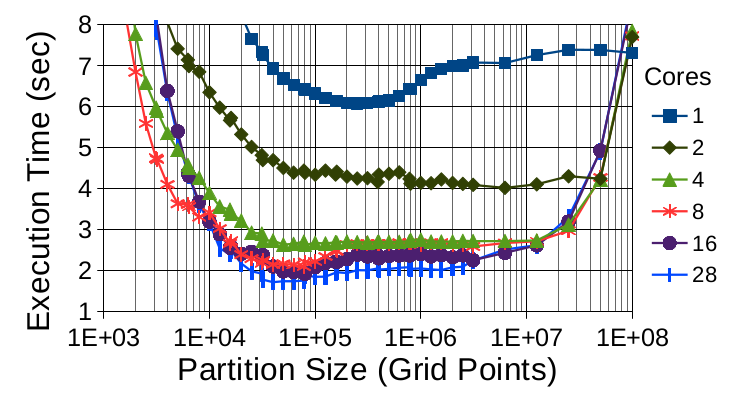
\includegraphics[scale=0.4]{images/task_granularity.png}
	\caption{The effect of task size on execution time for Stencil application \cite{grubel2015performance}}	
	\label{fig_task_gran}
\end{figure}

%\vspace{\baselineskip}
%\section{Modeling performance}
%Gunther states the factors involved in creating overheads as, exchanging data between memory and processors, waiting for completion of a memory access or an I/O, 
%\begin{itemize}
%	\item 
%	\item
%\end{itemize}



\vspace{\baselineskip}
\subsection{Universal Scalibility Law}
Amdahl's law\cite{amdahl1967validity}, states that the amount of achievable speed up by adding more processors when running a parallel application, is restricted by the amount of code that could actually be parallelized. 
Equation \ref{Amdahl}, shows the relationship between speedup and number of processors, where $\sigma$ is the serial fraction of the execution time, based on Amdahl's law\cite{gunther2007guerrilla}. 

\begin{equation}\label{Amdahl}
S(p) = \frac{p}{1+\sigma(p-1)}\\
\end{equation}

On the other hand, Gunther\cite{gunther2007guerrilla} extends Amdahl's law by incorporating the effect of three factors, namely concurrency, contention, and coherency, as shown in Equation~\ref{USL}.

\begin{equation}\label{USL}
S(p) = \frac{p}{1+\sigma(p-1)+\kappa{p}(p-1)}\\
\end{equation}

Concurrency($p$) represents the linear speedup that could have been achieved if no interaction existed among the processors, contention($\sigma$) represents the serialization effect of shared writable data, and finally coherency or data consistency($\kappa$) represents the effort that needs to be made for keeping shared writable data consistent\cite{gunther2007guerrilla}.    

Figure~\ref{fig_Amdahl} shows an example of the ideal linear speedup we expect to see when increasing the number of the processors, against the actual achievable speedup based on Amdahl's law and USL.

Equation~\ref{USL_generalized} generalizes Equation~\ref{USL} to represent the throughput by adding another parameter($\gamma$) to represent the serial throughput.

\begin{equation}\label{USL_generalized}
X(p) = \frac{\gamma{p}}{1+\sigma(p-1)+\kappa{p}(p-1)}\\
\end{equation}

\begin{figure}[H]
	\centering
	\includegraphics[width=1\linewidth]{images/Amdahls.png}
	\caption{An example of the achievable speedup based on Amdahl's law and USL compared to the ideal linear speedup where $\sigma=0.04$ and $\kappa=0.005$.}	
	\label{fig_Amdahl}
\end{figure}

Universal scalibility law also suggests that for some values of $\sigma$ and $\kappa$ there could be a certain number of processors that yield to maximum performance\cite{gunther2007guerrilla}. Increasing the number of processor beyond that point would only cause performance degradation.  

\vspace{\baselineskip}
\subsection{Other Models}	
There are a few other models that have also been suggested to simulate the scalibility. Geometric model is a one-parameter model, in which speedup has the following relationship with number of processors:
\begin{equation}\label{geo}
X(p) = \frac{1-\phi^{p}}{1-\phi}\\
\end{equation}

Exponential model
\begin{equation}\label{expo}
X(p) = \frac{1-\phi^{p}}{1-\phi}\\
\end{equation}

Quadratic model
\begin{equation}\label{quad}
X(p) = \frac{1-\phi^{p}}{1-\phi}\\
\end{equation}
\pagebreak
\singlespacing

\chapter{Literature Review}\label{Literature}
\doublespacing
\section{Literature Review}

Loop scheduling techniques has been extensively studied by different researchers. In \cite{donfack2012hybrid} the authors propose a hybrid static/dynamic method for loop scheduling that improves the performance of dense matrix factorization, compared to both fully static and fully dynamic scheduling. The authors of \cite{donfack2012hybrid}, divide the dependency graph into two subgraphs, one of which is scheduled dynamically and the other one is scheduled statically. The tasks on the critical path are scheduled statically and each thread is forced to prioritize the static tasks\cite{donfack2012hybrid}. They were able to improve data locality and scheduling overhead, while creating a more balanced workload. 

%\cite{xue2007locality}
% \cite{tang1986processor},\cite{polychronopoulos1987guided},\cite{hummel1992factoring},\cite{kruskal1985allocating}
%	

The previous work on predicting the performance of a parallel application mainly focuses on three major types of models: analytical, trace-based, and empirical models\cite{malakar2018benchmarking}. 

The analytical models\cite{blagojevic2008modeling},\cite{kerbyson2001predictive},\cite{valiant1990bridging}, while providing an arithmetic formula to represent the execution time of an application, require a deep understanding of the application, to apply platform-specific optimizations, and can not be generalized to different domains and architectures\cite{lee2007methods},\cite{sun2017automated},\cite{pllana2007performance}.
Traced-based models, on the other hand, use the traces collected through instrumentation, to predict the performance. These models, opposed to analytical models, do not rely on an expert's knowledge of the application, but while adding some overhead to the runtime, these models require a large storage space to save the traces, and are hard to interpret\cite{sun2017automated}.   
In empirical modeling, the results obtained from running an application with a set of parameters on a specific set of machines to build a model for unknown set of application and system parameters\cite{malakar2018benchmarking}. This type of modeling includes machine learning based approaches.

In \cite{ipek2005approach}, the authors use neural networks to predict the performance focusing on SMG2000 application, a parallel multigrid solver for linear systems\cite{falgout2002hypre}, on two different platforms. Defining application parameters $N_x$, $N_y$, $N_z$, representing the working set size per processor, and $P_x$, $P_y$, $P_z$, describing the three-dimension processor topology, as the features, \cite{ipek2005approach} uses a fully connected neural network to learn the model. Since they use absolute mean square error as the loss function, they use stratification to replicate samples with lower values by a factor which is proportional to their target value. They also apply bagging technique to decrease the variance in the model. As they increase the size of the training set to 5K points, they reach an error rate of 4.9\%. 

As a trace-based model, \cite{sun2017automated} analyzes the abstract syntax tree of the code and collects data through inserting special code for instrumentation when encounters 4 different situations, namely, assignments, branches, loops, and MPI communications. The authors then use 5 different machine learning methods including random forests, support vector machine, and ridge regression to build a prediction model from the collected data. Through applying two filtration processes, they were able to decrease the amount of overhead introduced along with the storage space requirement. Their results were inclined towards random forest, mainly because of the lower impact of categorical features on it, which is helpful in general cases where we do not have any knowledge about the type of features\cite{sun2017automated}.  
	
In \cite{malakar2018benchmarking} the authors investigate a set of machine learning techniques, including deep neural networks, support vector machine, decision tree, random forest, and k-nearest neighbor to predict the execution time of 4 different applications. Each of these applications require a certain set of features as input, for example, for the miniMD application in molecular dynamics, the number of processes and the number of atoms were considered as the input features, while for miniAMR, an application for studying adaptive mesh refinement, number of processes and also block sizes in $x$, $y$, and $z$ direction, where used as the input features. While achieving promising results especially for deep neural networks, bagging, and boosting methods, \cite{malakar2018benchmarking} suggest utilizing transfer learning through deep neural networks to predict performance on other platforms.
%	
%\cite{pusukuri2011thread}
%\cite{marin2004cross}

Although concentrating on GPUs,	\cite{liu2018runtime} proposes a lightweight machine learning based performance model to choose the number of threads to use for parallelization for a specific data size and operation. With the final goal of improving the training time in a neural network, \cite{liu2018runtime} selects 4 performance features collected by hardware counters namely, number of CPU cycles, number of cache misses, cache accesses for the last cache level, and number of level 1 cache hits. Then they take two different approaches to build their model. In the first on they try 10 different regression models including random forest, and in the second one they use hill climbing algorithm to choose the number of threads. In addition to hardware independent, and not requiring the training process, hill climbing algorithm achieves a much higher accuracy compared to the best performing regression model.

In this paper, we suggest using machine learning to directly predict the optimal chunk size to achieve the best performance instead of predicting the execution time or the optimal number of cores to run the application on. For this purpose, we have offered a set of general features that are not specific to an application and could easily be extracted at compile time or at run time. Once the data has been collected and our model has been created, the prediction results could be easily applied to a new application with a negligible overhead. 

%\cite{sun2017automated}
As another field to use machine learning, \cite{qawasmeh2015adaptive} collects seven runtime events and uses machine learning not to predict the performance, but to schedule the tasks. These events include, task creation, suspension, execution, completion, implicit/explicit barrier, parallel region, and finally loop/master/single region runtime events, collected through the OMPT using ORA API. Experimenting with four different machine learning techniques, including support vector machine, random forest, neural networks, and naive bayes, they would select one specific task pool configuration out of the three pre-defined options as the final classification result. Testing this framework on a real life molecular dynamics application, they observed an up to 31\% improvement in performance. 
%Compiler-based methods:

The authors of \cite{wang2009mapping} propose using machine learning to predict the optimal number of threads, and also the optimal scheduling policy for running an OpenMP application. Through that, they were able to develop an automatic compiler-based method to map a parallel application to a multicore processor. They collect three type of features namely, code, data, and runtime features. Code features are extracted from the code directly, and they include cycles per instruction, number of branches, load and store instructions, and computations per instruction. While the code features could be collected statically at compile time, the data and run-time features are collected through low-cost profiling runs. This group of features include loop iteration count, branch miss rate, and $L1$ data cache miss rate. The authors of \cite{wang2009mapping} then use an artificial neural network to predict the speedup achieved for a program with certain number of threads, and at the same time they use a support vector machine model to predict the best scheduling policy, out of block, cyclic, dynamic, and guided scheduling policies, for an unseen program.



	
	
	
	
%\cite{treibig2012performance} 
%profiling information about the application on a given architecture
%\cite{cammarota2012just},\cite{zhang2005runtime},\cite{thoman2012automatic}
%
%Machine learning models 
%\cite{singh2009real}, \cite{zomaya2001observations}, \cite{qawasmeh2015adaptive}
%
%
%
%	
%
%	
%
%\cite{li2009machine}
\vspace{\baselineskip}



\pagebreak
\singlespacing

\chapter{Method}\label{Method}
\doublespacing
%In this section we discuss how and for what purpose the HPX backend for Blaze was modified. Our work here heavily depends on the data.
\vspace{\baselineskip}	
\section{Parallelization in Blaze}
Depending on the operation and the size of operands, this assignment could be parallelized through four different backends, namely, HPX, OpenMP\cite{dagum1998openmp}, C++ threads, and Boost\cite{Boost}. 
Table~\ref{table2} shows the default value for some of the threshold for parallelization applied to operations performed in Blaze. It should be noted that these thresholds should be tuned based on the parallelization backend and also the system architecture.
%For matrix matrix multiplication alongside the mentioned thresholds, there exists another set of thresholds to switch between using Blaze kernels or BLAS kernels. 
%As stated in Section~\ref{Background} Blaze being based on smart expression templates, offers the option to use either Blaze or a highly optimized kernel for computations. This option is set at compile time through $BLAS_mode$ macro. If $BLAS_mode=1$, 

\vspace{\baselineskip}	
\begin{table}[H]
	\centering
	\resizebox{\textwidth}{!}
	{\begin{tabular}{|c | c |} 
			\hline
			Benchmark & Array size \\ [0.5ex] 
			\hline
			\hline
			$DVECDVCEADD$, $DVECDVECMULT$ & 38000\\ 	
			\hline
			$DMATDMATADD$ & 36100 elements equivalent to a $175\times{175}$ matrix \\
			\hline	
			$DMATDMATMULT$ & 3025 elements equivalent to a $55\times{55}$ matrix  \\
			\hline			
	\end{tabular}}
	
	\caption{List of some of the thresholds applied to the operations performed by Blaze, starting from which the operation is executed in parallel}
	\label{table2}
\end{table} 

\vspace{\baselineskip}	
\subsection{Implementation of HPX Backend}
As stated earlier, as an ET-based library, blaze performs the calculations when an expression is assigned to a target, which is implemented through the \textit{blaze::Assign} function.

The four mentioned backends, parallelize this assignment process through a parallel for-loop, in which at each iteration a specific section of each of the vectors or matrices(called a block) is selected and assigned to a core. Each core then performs the operation on the block they have been assigned to.  

Each backend uses their own method for parallelizing this for loop. For HPX backend, current implementation uses a HPX \textit{parallel::for\textunderscore loop} with static chunking policy and chunk size of 1. This way, knowing the number of cores to run the application on, we can divide the original matrix equally among the cores, while the order of assignment of blocks to the cores is known at compile time.  
Listings\ref{old_hpx_backend} shows the current implementation of the HPX backend in Blaze.

\begin{lstlisting}[basicstyle=\fontsize{8}{9}\selectfont,float,floatplacement=H,caption= {Previous implementation of Assign function for HPX backend in Blaze.}, label={old_hpx_backend}]
template< typename MT1   // Type of the left-hand side dense matrix
, bool SO1       // Storage order of the left-hand side dense matrix
, typename MT2   // Type of the right-hand side dense matrix
, bool SO2       // Storage order of the right-hand side dense matrix
, typename OP >  // Type of the assignment operation
void hpxAssign( DenseMatrix<MT1,SO1>& lhs, const DenseMatrix<MT2,SO2>& rhs, OP op )
{
using hpx::parallel::for_loop;
using hpx::parallel::execution::par;

BLAZE_FUNCTION_TRACE;

using ET1 = ElementType_t<MT1>;
using ET2 = ElementType_t<MT2>;

constexpr bool simdEnabled( MT1::simdEnabled && MT2::simdEnabled && IsSIMDCombinable_v<ET1,ET2> );
constexpr size_t SIMDSIZE( SIMDTrait< ElementType_t<MT1> >::size );

const bool lhsAligned( (~lhs).isAligned() );
const bool rhsAligned( (~rhs).isAligned() );

const size_t threads    ( getNumThreads() );
const ThreadMapping threadmap( createThreadMapping( threads, ~rhs ) );

const size_t addon1     ( ( ( (~rhs).rows() % threadmap.first ) != 0UL )? 1UL : 0UL );
const size_t equalShare1( (~rhs).rows() / threadmap.first + addon1 );
const size_t rest1      ( equalShare1 & ( SIMDSIZE - 1UL ) );
const size_t rowsPerThread( ( simdEnabled && rest1 )?( equalShare1 - rest1 + SIMDSIZE ):( equalShare1 ) );

const size_t addon2     ( ( ( (~rhs).columns() % threadmap.second ) != 0UL )? 1UL : 0UL );
const size_t equalShare2( (~rhs).columns() / threadmap.second + addon2 );
const size_t rest2      ( equalShare2 & ( SIMDSIZE - 1UL ) );
const size_t colsPerThread( ( simdEnabled && rest2 )?( equalShare2 - rest2 + SIMDSIZE ):( equalShare2 ) );

for_loop( par, size_t(0), threads, [&](int i)
{
const size_t row   ( ( i / threadmap.second ) * rowsPerThread );
const size_t column( ( i % threadmap.second ) * colsPerThread );

if( row >= (~rhs).rows() || column >= (~rhs).columns() )
return;

const size_t m( min( rowsPerThread, (~rhs).rows()    - row    ) );
const size_t n( min( colsPerThread, (~rhs).columns() - column ) );

if( simdEnabled && lhsAligned && rhsAligned ) {
auto       target( submatrix<aligned>( ~lhs, row, column, m, n ) );
const auto source( submatrix<aligned>( ~rhs, row, column, m, n ) );
op( target, source );
}
else if( simdEnabled && lhsAligned ) {
auto       target( submatrix<aligned>( ~lhs, row, column, m, n ) );
const auto source( submatrix<unaligned>( ~rhs, row, column, m, n ) );
op( target, source );
}
else if( simdEnabled && rhsAligned ) {
auto       target( submatrix<unaligned>( ~lhs, row, column, m, n ) );
const auto source( submatrix<aligned>( ~rhs, row, column, m, n ) );
op( target, source );
}
else {
auto       target( submatrix<unaligned>( ~lhs, row, column, m, n ) );
const auto source( submatrix<unaligned>( ~rhs, row, column, m, n ) );
op( target, source );
}
} );
}
\end{lstlisting}

What we suggest here is that, some prior knowledge for example, architecture of the system we are running the application on, the expression that has to be executed, number of cores of the system, size and type of the arrays we are dealing with, and etc. should be able to help us to achieve a higher performance.
For this purpose we introduced two parameters block\textunderscore{size} and chunk\textunderscore{size}.

\begin{lstlisting}[basicstyle=\fontsize{8}{9}\selectfont,float,floatplacement=H,caption= {New implementation of Assign function for HPX backend in Blaze.}, label={new_hpx_backend}]
template< typename MT1   // Type of the left-hand side dense matrix
, bool SO1       // Storage order of the left-hand side dense matrix
, typename MT2   // Type of the right-hand side dense matrix
, bool SO2       // Storage order of the right-hand side dense matrix
, typename OP >  // Type of the assignment operation
void hpxAssign( DenseMatrix<MT1,SO1>& lhs, const DenseMatrix<MT2,SO2>& rhs, OP op )
{
using hpx::parallel::for_loop;
using hpx::parallel::execution::par;

BLAZE_FUNCTION_TRACE;

using ET1 = ElementType_t<MT1>;
using ET2 = ElementType_t<MT2>;

constexpr bool simdEnabled( MT1::simdEnabled && MT2::simdEnabled && IsSIMDCombinable_v<ET1,ET2> );
constexpr size_t SIMDSIZE( SIMDTrait< ElementType_t<MT1> >::size );

const bool lhsAligned( (~lhs).isAligned() );
const bool rhsAligned( (~rhs).isAligned() );

const size_t threads    ( getNumThreads() );
const size_t numRows ( min( static_cast<std::size_t>( BLAZE_HPX_MATRIX_BLOCK_SIZE_ROW ), (~rhs).rows() ) );
const size_t numCols ( min( static_cast<std::size_t>( BLAZE_HPX_MATRIX_BLOCK_SIZE_COLUMN ), (~rhs).columns() ) );

const size_t rest1      ( numRows & ( SIMDSIZE - 1UL ) );
const size_t rowsPerIter( ( simdEnabled && rest1 )?( numRows - rest1 + SIMDSIZE ):( numRows ) );
const size_t addon1     ( ( ( (~rhs).rows() % rowsPerIter ) != 0UL )? 1UL : 0UL );
const size_t equalShare1( (~rhs).rows() / rowsPerIter + addon1 );

const size_t rest2      ( numCols & ( SIMDSIZE - 1UL ) );
const size_t colsPerIter( ( simdEnabled && rest2 )?( numCols - rest2 + SIMDSIZE ):( numCols ) );
const size_t addon2     ( ( ( (~rhs).columns() % colsPerIter ) != 0UL )? 1UL : 0UL );
const size_t equalShare2( (~rhs).columns() / colsPerIter + addon2 );

hpx::parallel::execution::dynamic_chunk_size chunkSize ( BLAZE_HPX_MATRIX_CHUNK_SIZE );

for_loop( par.with( chunkSize ), size_t(0), equalShare1 * equalShare2, [&](int i)
{
const size_t row   ( ( i / equalShare2 ) * rowsPerIter );
const size_t column( ( i % equalShare2 ) * colsPerIter );

if( row >= (~rhs).rows() || column >= (~rhs).columns() )
return;

const size_t m( min( rowsPerIter, (~rhs).rows()    - row    ) );
const size_t n( min( colsPerIter, (~rhs).columns() - column ) );

if( simdEnabled && lhsAligned && rhsAligned ) {
auto       target( submatrix<aligned>( ~lhs, row, column, m, n ) );
const auto source( submatrix<aligned>( ~rhs, row, column, m, n ) );
op( target, source );
}
else if( simdEnabled && lhsAligned ) {
auto       target( submatrix<aligned>( ~lhs, row, column, m, n ) );
const auto source( submatrix<unaligned>( ~rhs, row, column, m, n ) );
op( target, source );
}
else if( simdEnabled && rhsAligned ) {
auto       target( submatrix<unaligned>( ~lhs, row, column, m, n ) );
const auto source( submatrix<aligned>( ~rhs, row, column, m, n ) );
op( target, source );
}
else {
auto       target( submatrix<unaligned>( ~lhs, row, column, m, n ) );
const auto source( submatrix<unaligned>( ~rhs, row, column, m, n ) );
op( target, source );
}
} );
}
\end{lstlisting}
\vspace{\baselineskip}	
\subsection{HPX \textit{for\textunderscore loop}}
HPX \textit{for\textunderscore loop} takes an execution policy as first argument, which is set to \textit{dynamic\textunderscore chunk\textunderscore size} execution policy in case of HPX backend for Blaze.

\vspace{\baselineskip}	
\section{Experiments}
In order to capture the relationship between number of cores, \textit{chunk\textunderscore{size}}, \textit{block\textunderscore{size}}, and the performance, we ran a series of experiments with different of these parameters and measured the number of floating point operations per second performed. 

For these experiments ,at the first step we selected the $DMatDMatADD$ benchmark which was implemented in Blazemark. $DMatDMatADD$ benchmark is a level 3 BLAS function to perform matrix-matrix addition in the form of $A=B+C$, where $A$, $B$, $C$ are square matrices of the same size. For simplification we are only studying raw-major matrices at this point. Our final goal is to extend the work to cover arbitrary data layouts for arrays.

To avoid adding the scheduling overhead for small matrix sizes, Blaze uses a threshold to start parallelization, which is specific to the type of operation. For matrix-matrix addition, if the number of elements in the matrix is greater than 36100 elements(which is equivalent to a square matrix of size 190$\times$190) Blaze uses the configured backend to parallelize the assignment operation. For this reason, we start our experiments with matrix size of 200x200 and gradually increase the size to 1587$\times$1587. 
Table~\ref{table1} show the matrix sizes and the number of cores chosen for our experiments with $DMATDMATADD$ benchmark.

\vspace{\baselineskip}	
\begin{table}[H]
	\centering
		\resizebox{\textwidth}{!}
		{\begin{tabular}{|c | c |} 
			\hline
			Matrix sizes & 200, 230, 264, 300, 396, 455, 523, 600, 690, 793, 912, 1048, 1200, 1380, 1587 \\ [0.5ex] 
			\hline
			Number of cores & 1, 2, 3, 4, 5, 6, 7, 8 \\ 	
			\hline
			Number of rows in the block & 4, 8, 12, 16, 20, 32 \\
			\hline	
			Number of columns in the block & 64, 128, 256, 512, 1024 \\
			\hline
			Chunk size & Between 1 and total number of blocks (logarithmic increase)\\\hline
		\end{tabular}}

		\caption{List of different values used for each variable for running the $DMATDMATADD$ benchmark}
		\label{table1}
\end{table}

\vspace{\baselineskip}	
Figure~\ref{fig1} shows the results of running $DMatDMatADD$ benchmark for matrix sizes and number of cores listed in Tbale~\ref{table1} based on grain size. 

On the other hand, Figure~\ref{fig4} integrates the results obtained from running the same benchmark with different matrix sizes. Each color in this graph represents a specific matrix size. 

\vspace{\baselineskip}	
\begin{figure}[H]
	\centering
	\hspace*{-2cm}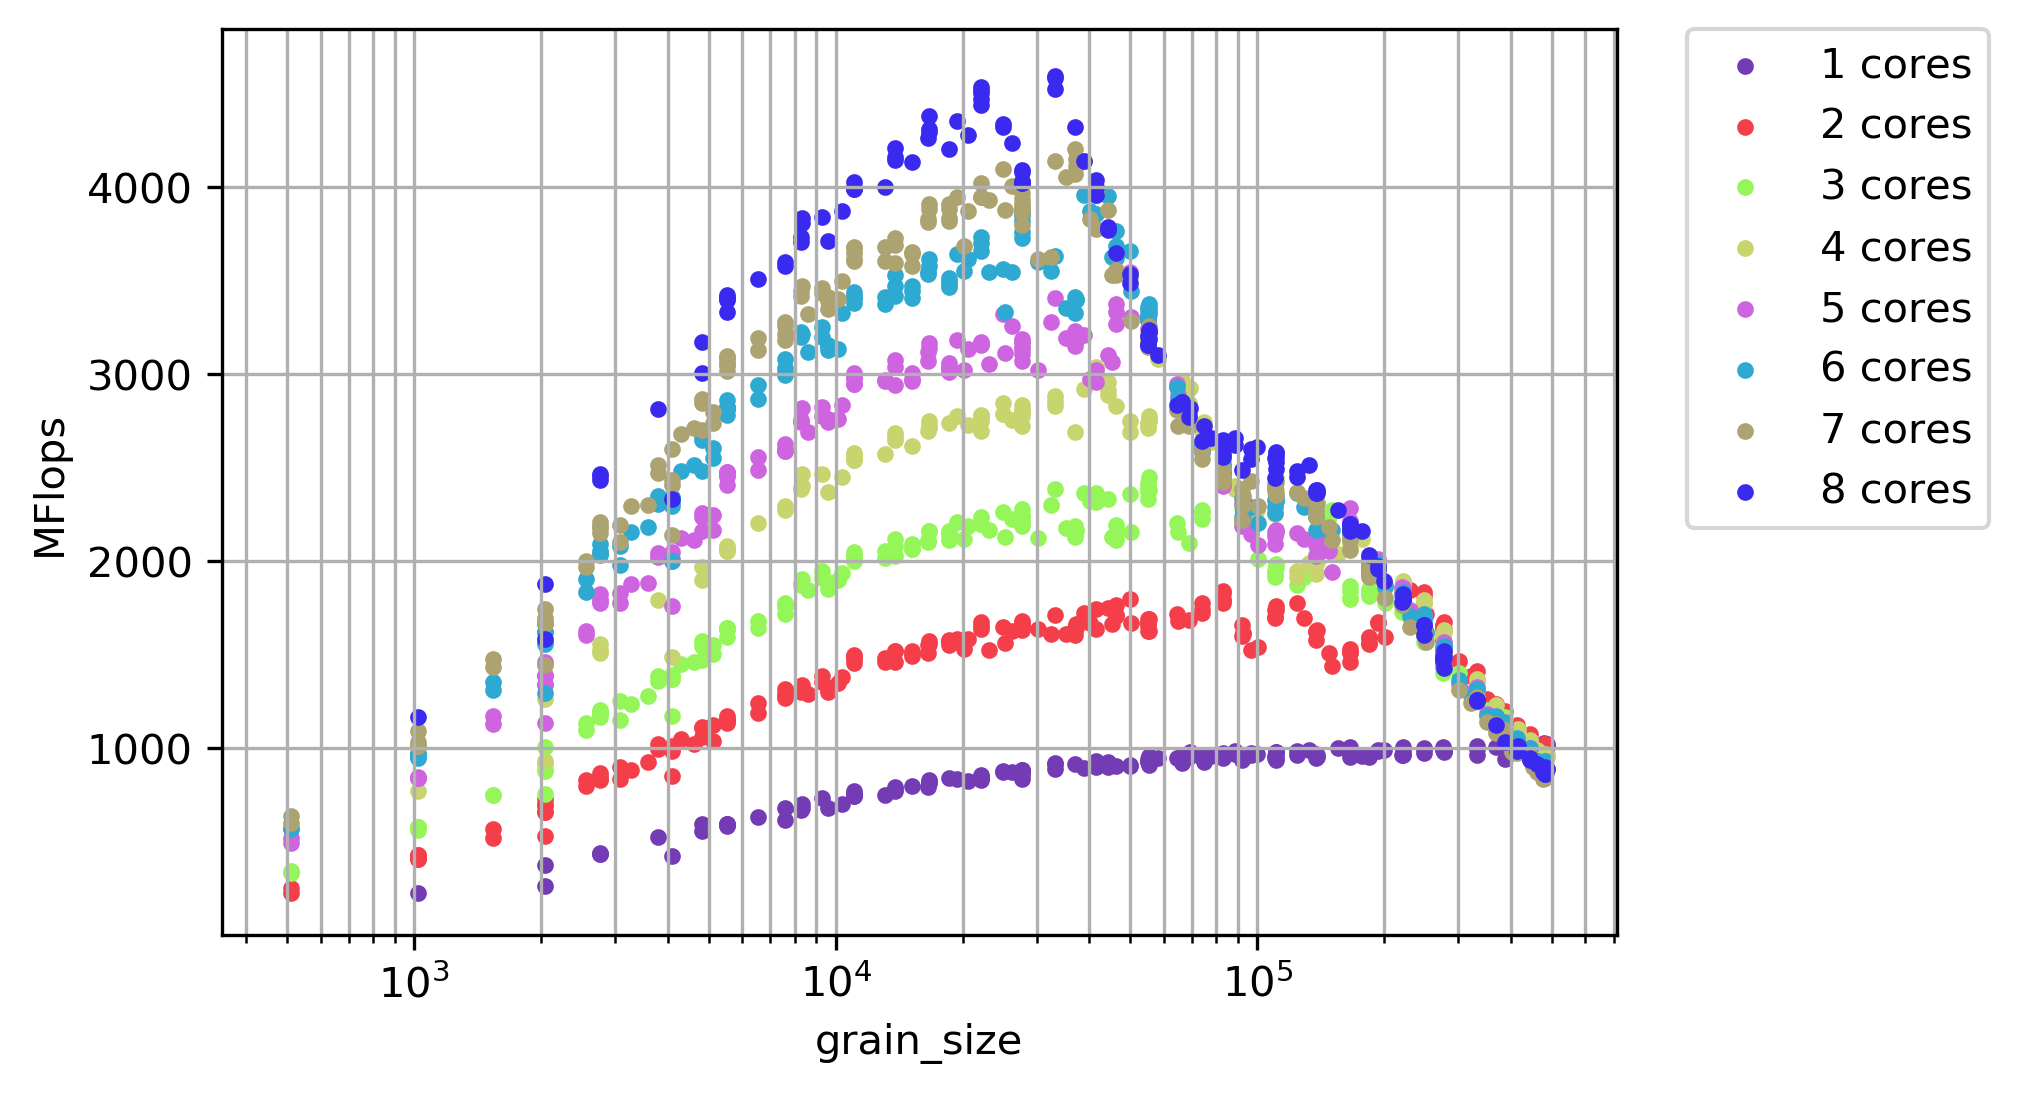
\includegraphics[scale=.75]{images/fig13.png}
	\caption{The results obtained from running $DMATDMATADD$ benchmark through Blazemark for matrix size 690$\times$690 on different number of cores.}	
	\label{fig9}
\end{figure}

\vspace{\baselineskip}	
\begin{figure}[H]
	\centering
	{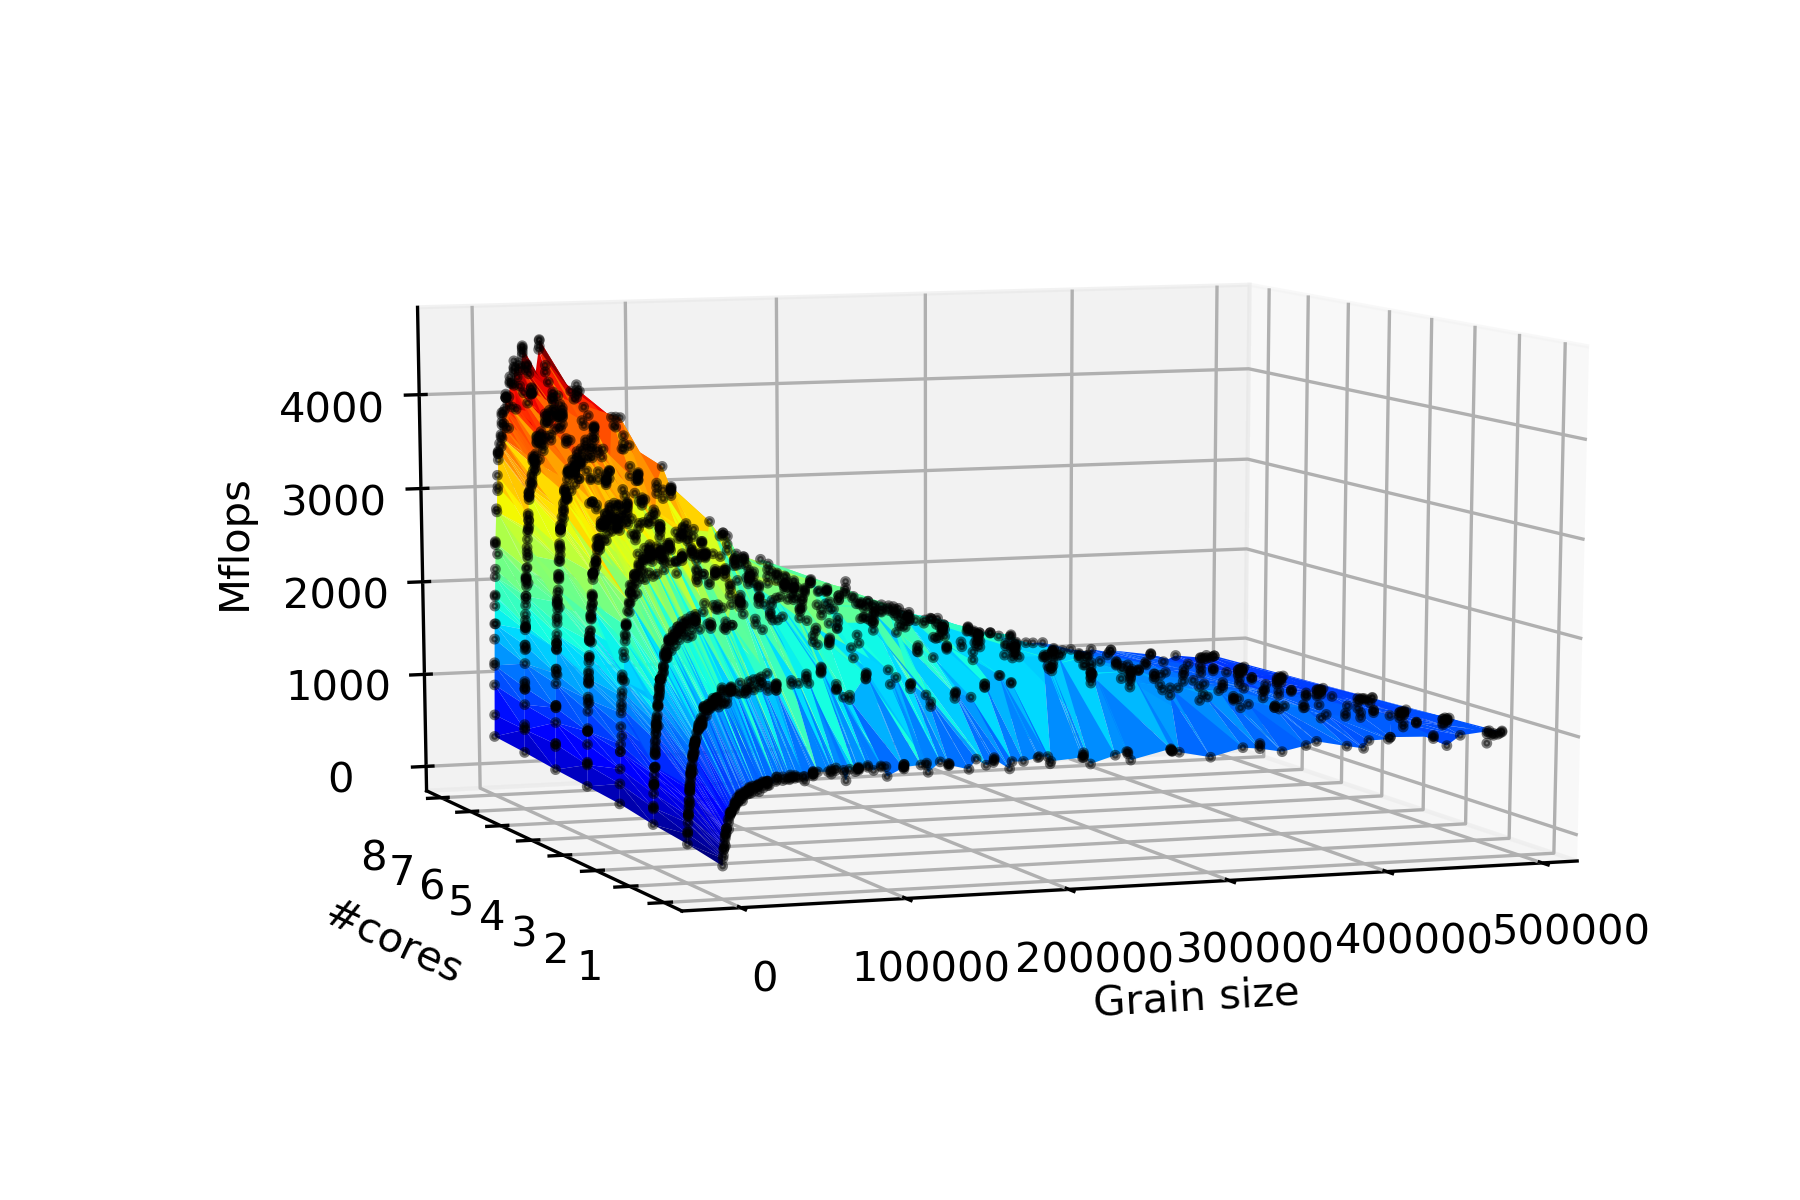
\includegraphics[scale=0.7]{images/fig2.png}}
	{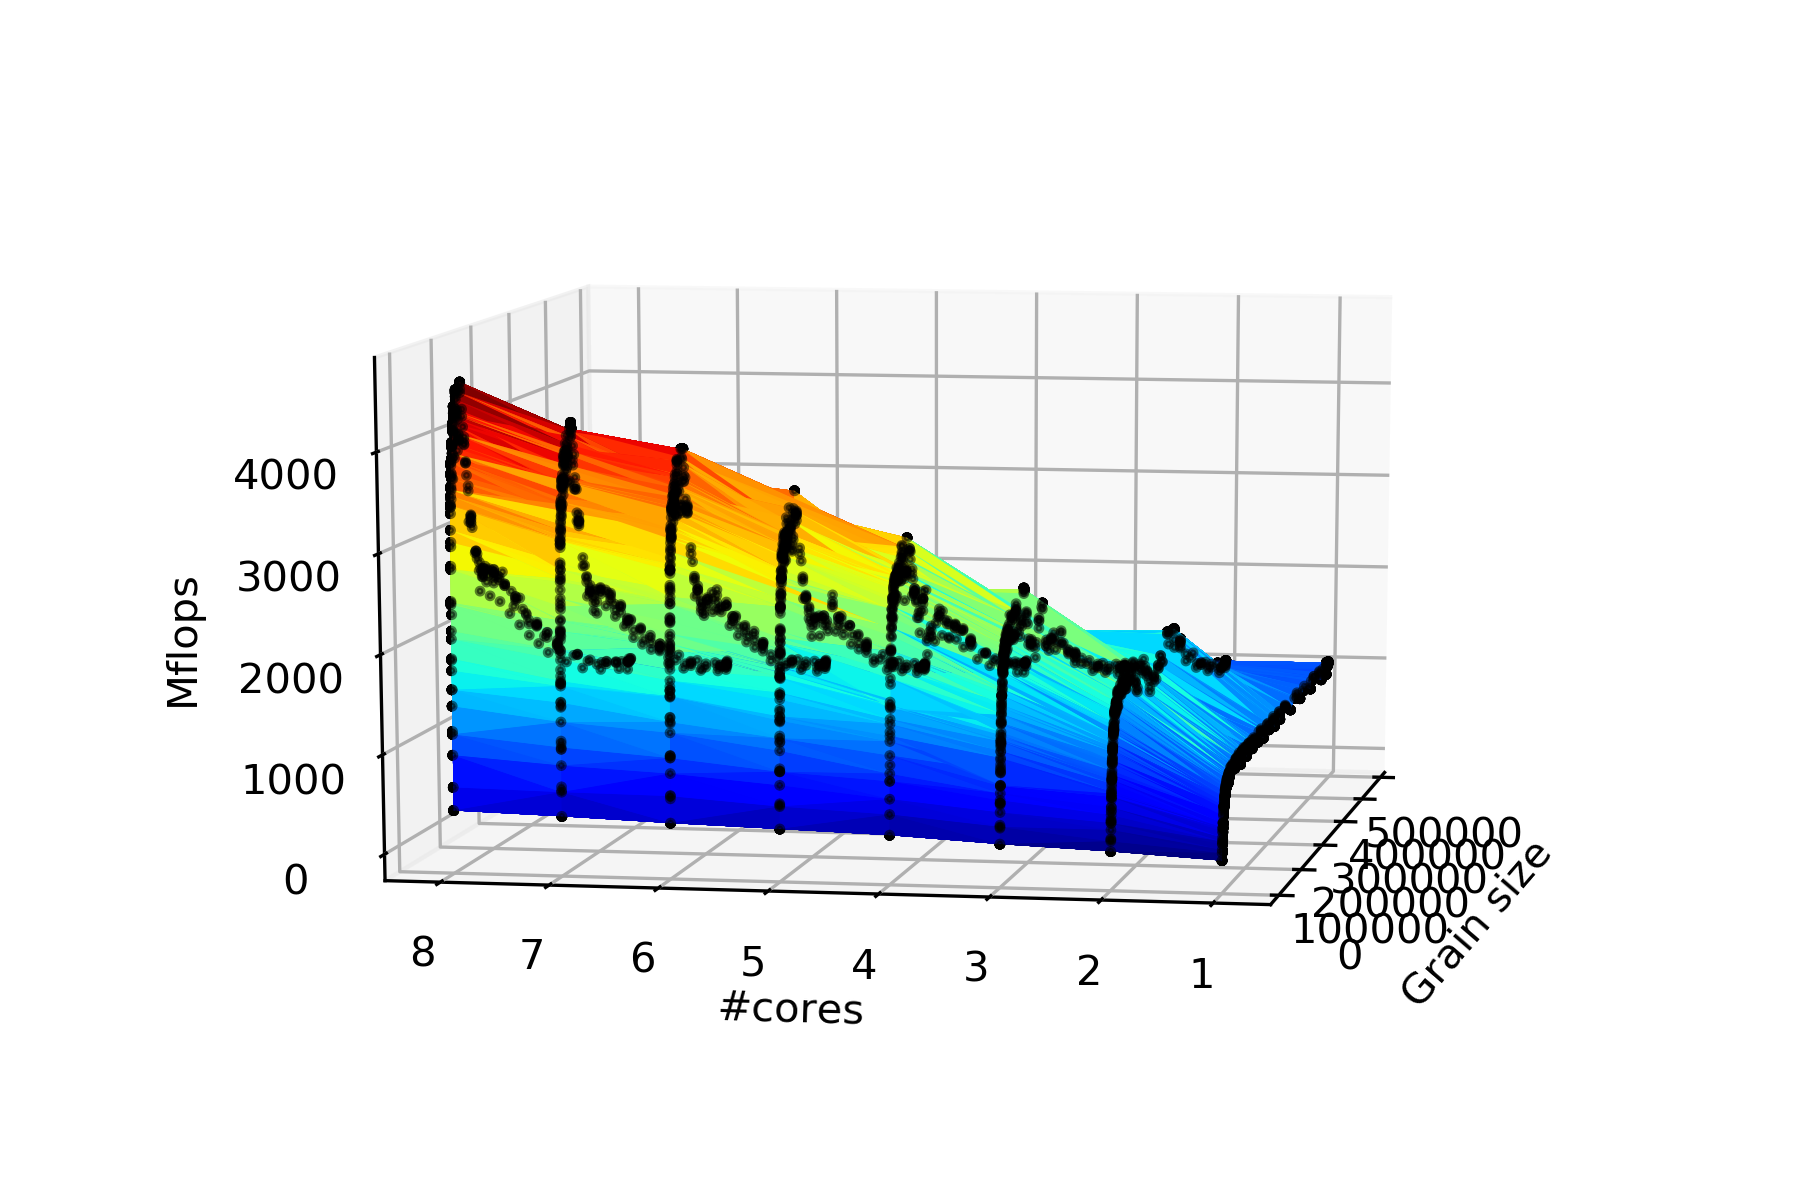
\includegraphics[scale=0.7]{images/fig3.png}}
	\caption{The results obtained from running $DMATDMATADD$ benchmark through Blazemark for matrix of size 690$\times$690 from two different angles}	
	\label{fig1}
\end{figure}

\begin{figure}[H]
	\centering
	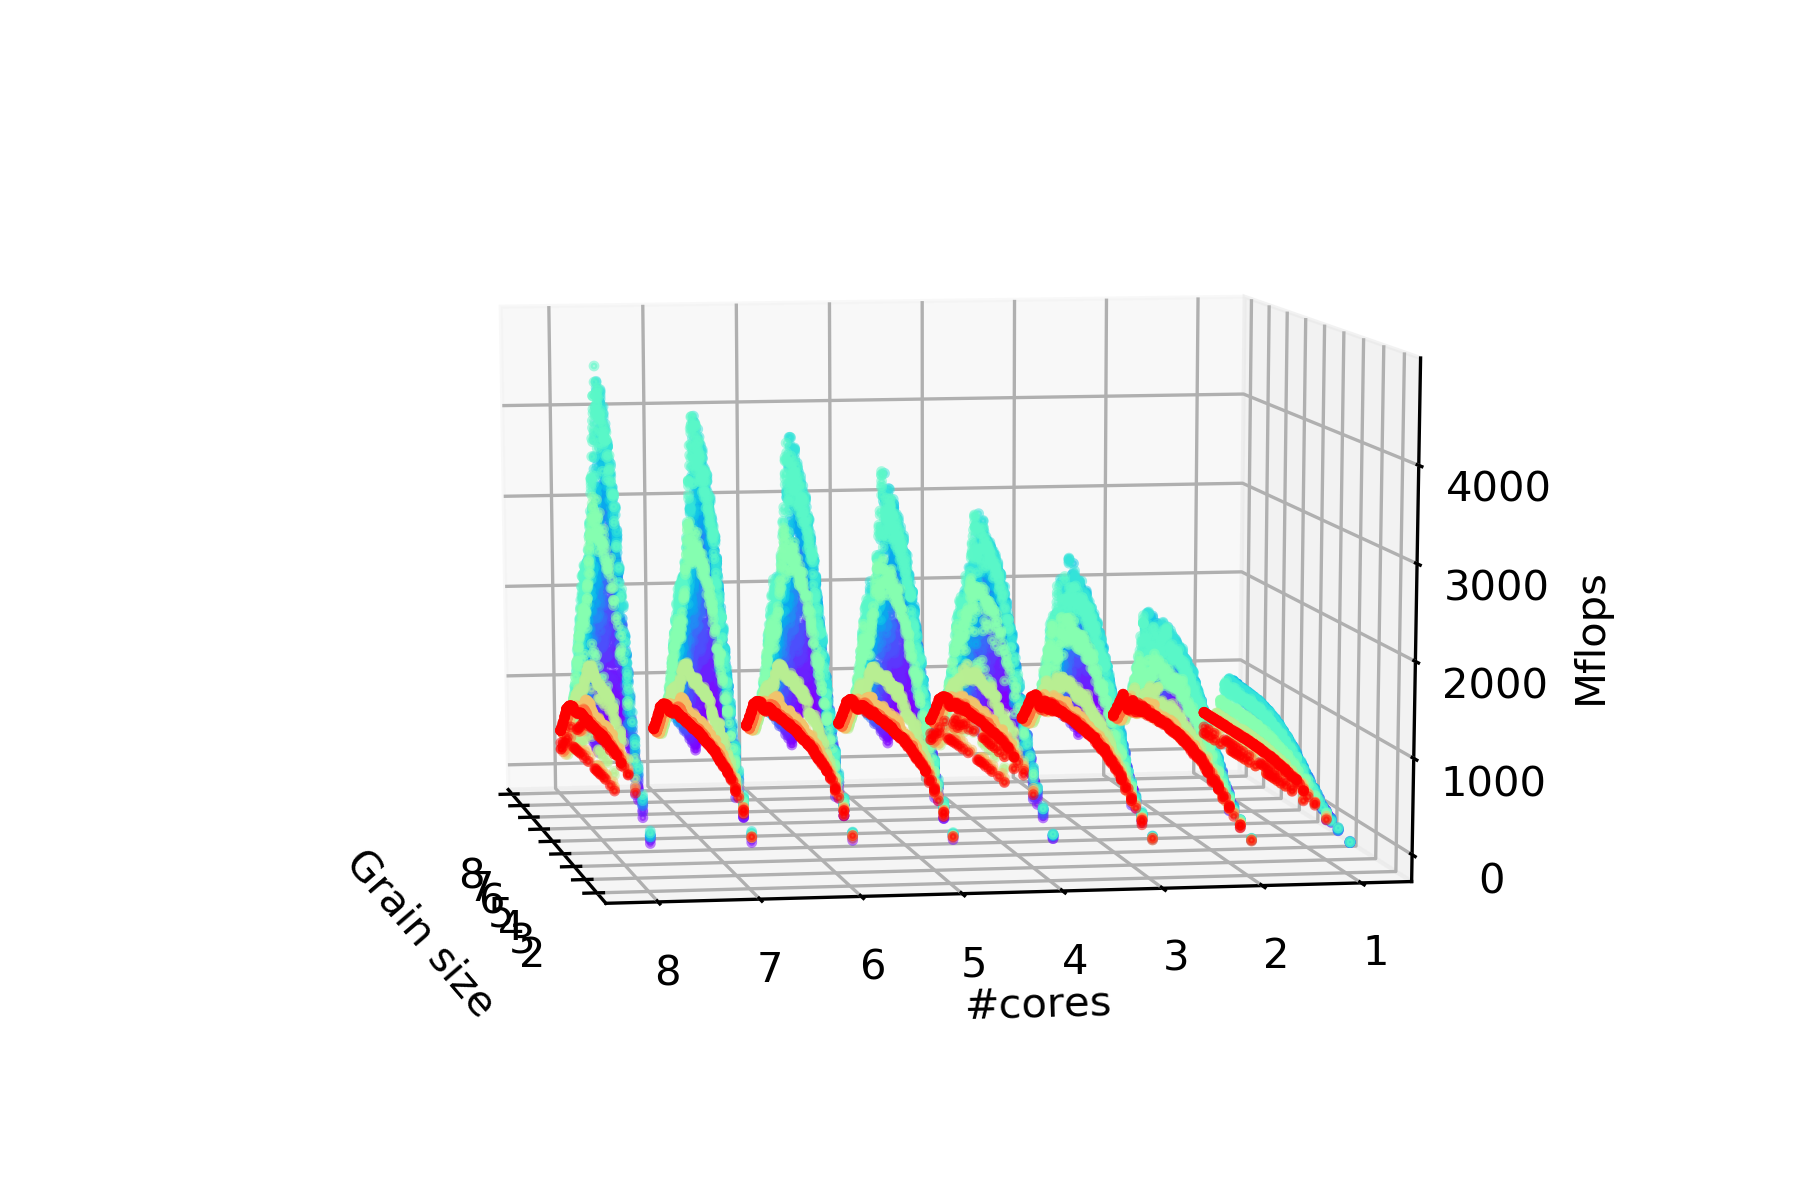
\includegraphics[width=1\linewidth]{images/fig4.png}
	\caption{The results obtained from running $DMATDMATADD$ benchmark through Blazemark for matrix sizes from 200$\times$200 to 1587$\times$1587}	
	\label{fig4}
\end{figure}

\vspace{\baselineskip}	
\subsection{Observation}
The final purpose of our experiments is to find a chunk size that gives us the best performance for a given matrix size on a given machine. This chunk size should also be tailored to the expression being executed, and this all is based on assuming that we have already fixed the block size.
So the first step appeared to be selecting the block size. For this purpose, we ran the experiments with a selection of block sizes as shown in Table~\ref{table1}.


It should be mentioned that there were three constraints on selecting the block sizes. First, Blaze forces the number of columns in a raw-major matrix to be divisible to SIMD register size in order to be able to take advantage of vectorization. Second, we have selected the number of columns in our blocks to be either divisible by cache line or to contain all the columns of the matrix.     


\begin{figure}[H]
	\centering
	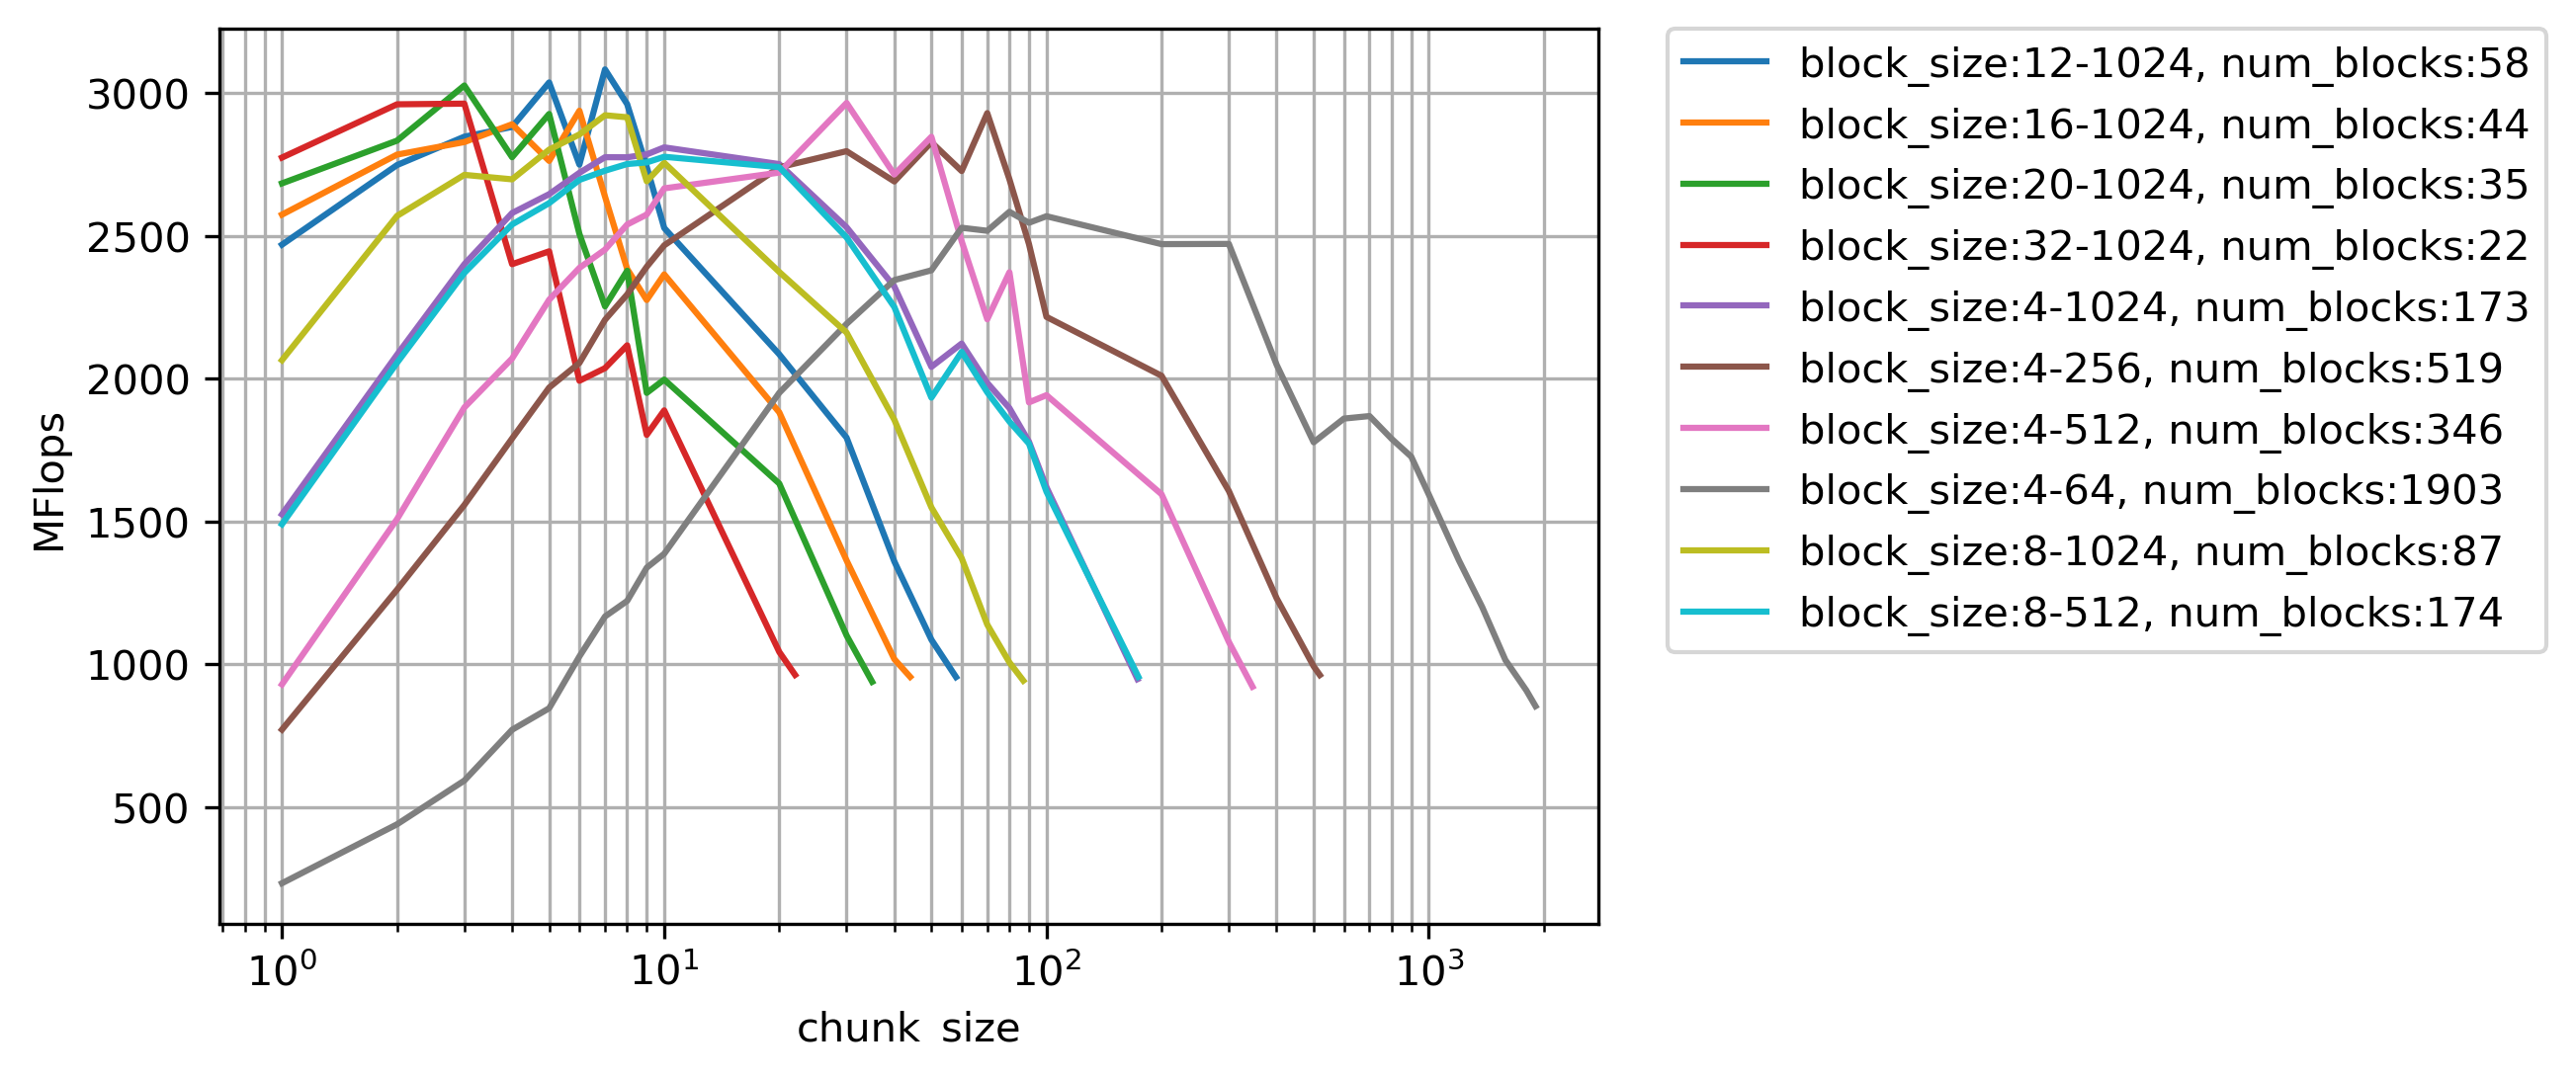
\includegraphics[width=1\linewidth]{images/fig5.png}
	\caption{The results obtained from running $DMATDMATADD$ benchmark through Blazemark for matrix sizes from 690$\times$690 with different combinations of block size and chunk size on $4$ cores}	
	\label{fig5}
\end{figure}

The collected data, as seen in Figure~\ref{fig5}, suggests two main points:
\begin{itemize}
	\item For each selected block size, there is a range of chunk sizes that gives us the best performance. 
	\item Except for some uncommon cases, no matter which block size we choose, we are able to achieve the maximum performance if we select the right chunk size.  
\end{itemize}

This motivated us to move our search parameter from chunk size to grain size. As stated earlier, grain size is the amount of work assigned to one HPX thread. Here we represent grain size by number of floating point operations performed by a HPX thread. For example, performing addition among two matrices, if we choose the block size as $4\times64$ and chunk size as $3$, the grain size would be $3\times4\times64=768$. 
Note that in our experiments whenever the number of columns of the original matrix is not divisible to the selected number of columns for block size, there would be a set of blocks with less number of elements than the selected block size, this has been considered when calculating the grain size.  

By changing our focus to the grain size instead of the block size and the chunk size, Figure~\ref{fig6} shows how the throughput changes with regards to the grain size for the $DMATDMATADD$ benchmark, for each specific block size. Each combination of block size and chunk size generates a point in the graph. On the other hand, Figure~\ref{fig9} looks at these graphs from another aspect, keeping the problem size constant but changing the number of the cores to run the benchmark on, instead.

\begin{figure}[H]
	\centering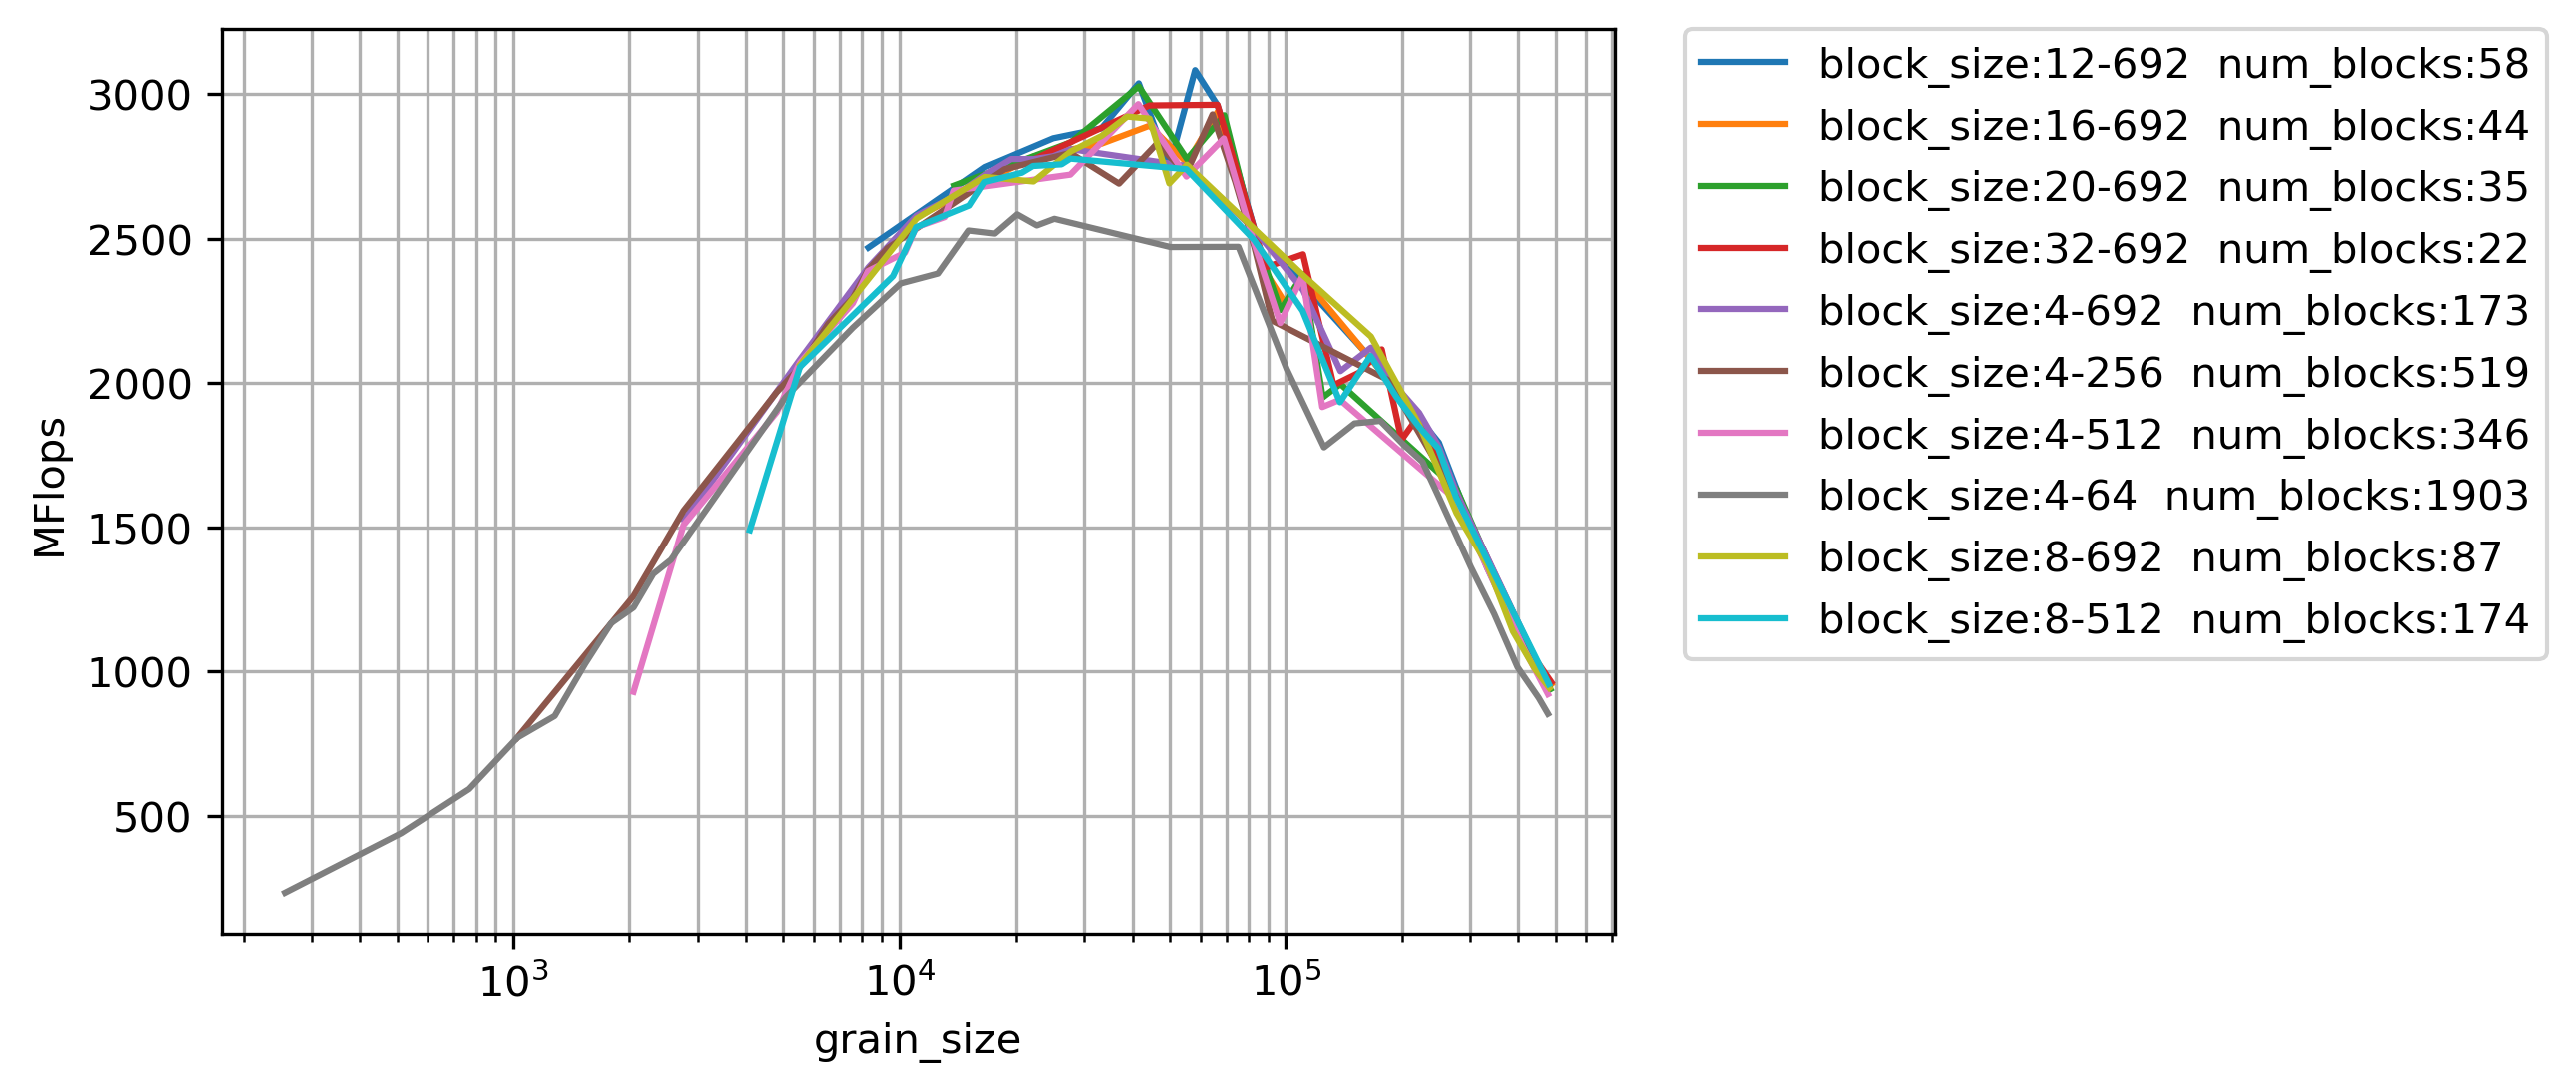
\includegraphics[width=1\linewidth]{images/fig6.png}
	\caption{The results obtained from running $DMATDMATADD$ benchmark through Blazemark for matrix size 690$\times$690 on $4$ cores.}	
	\label{fig6}
\end{figure}

%\begin{figure}[H]
%	\centering
%	\hspace*{-2cm}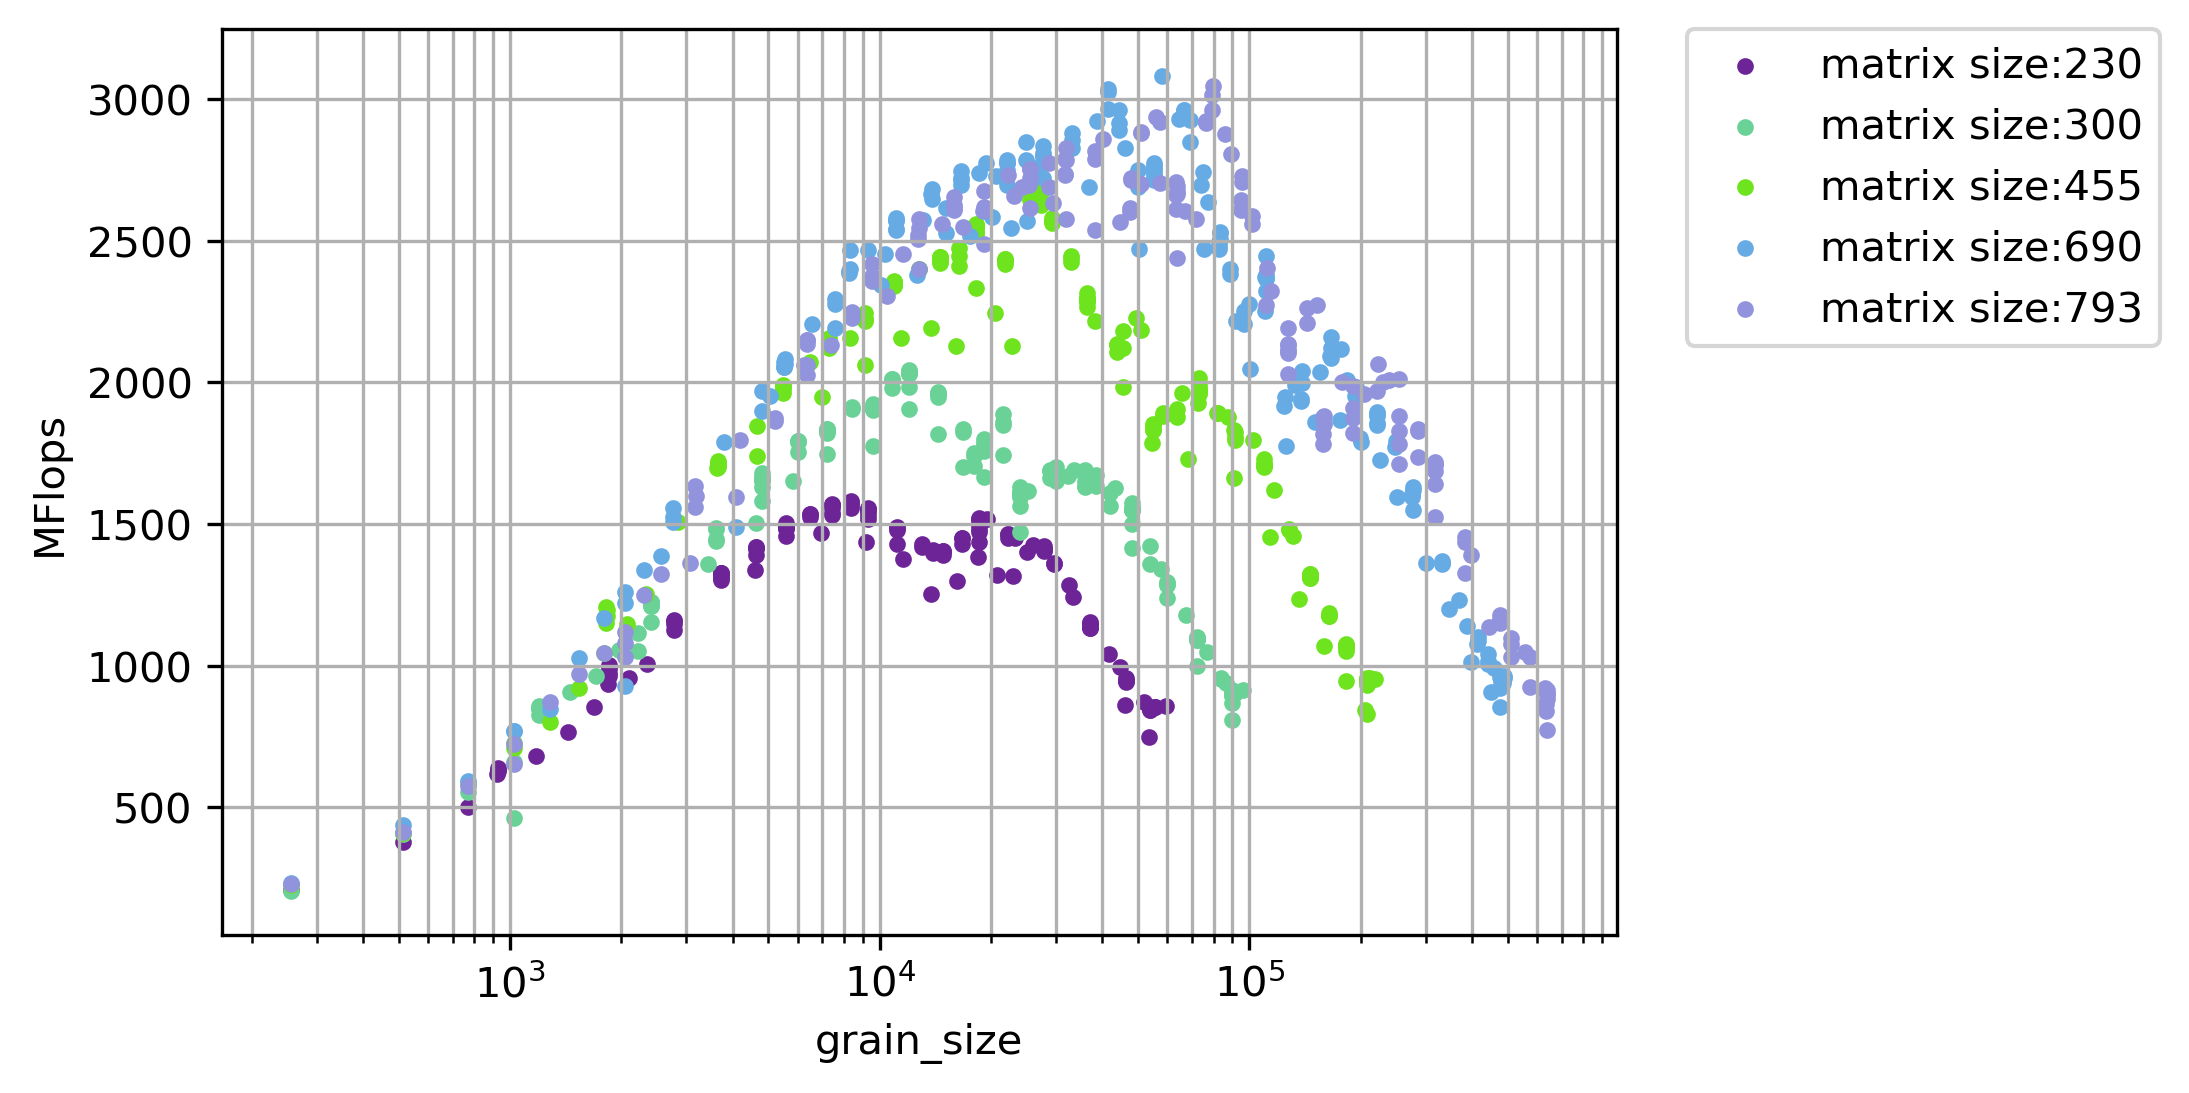
\includegraphics[scale=.75]{images/fig8.png}
%	\caption{The results obtained from running $DMATDMATADD$ benchmark through Blazemark for 5 different matrix sizes on $4$ cores.}	
%	\label{fig7}
%\end{figure}

\begin{figure}
	\subfloat[]
	{\centering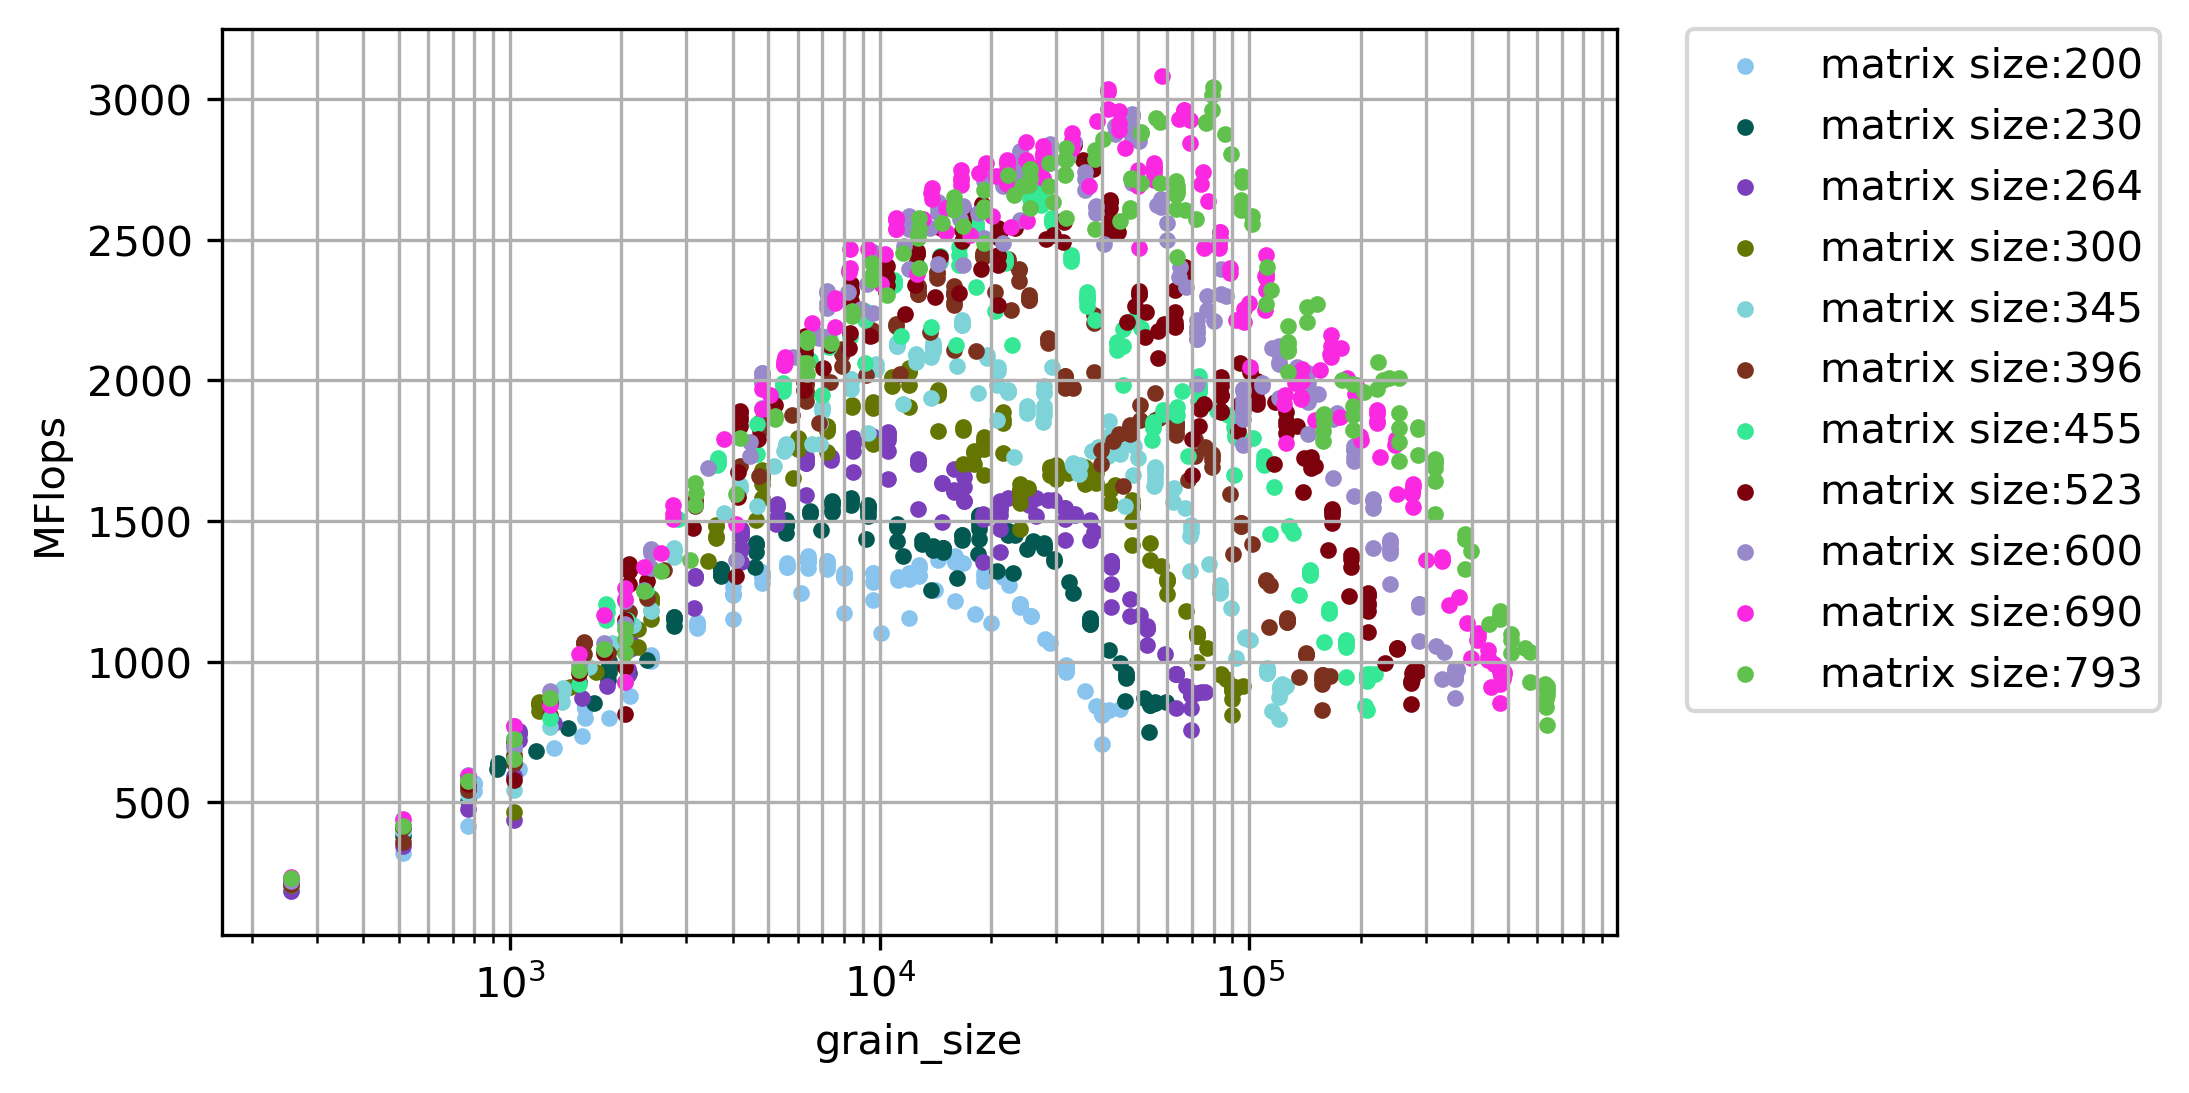
\includegraphics[scale=.75]{images/fig11.png}	
	\label{fig8:a}}

	\subfloat[]{
	\centering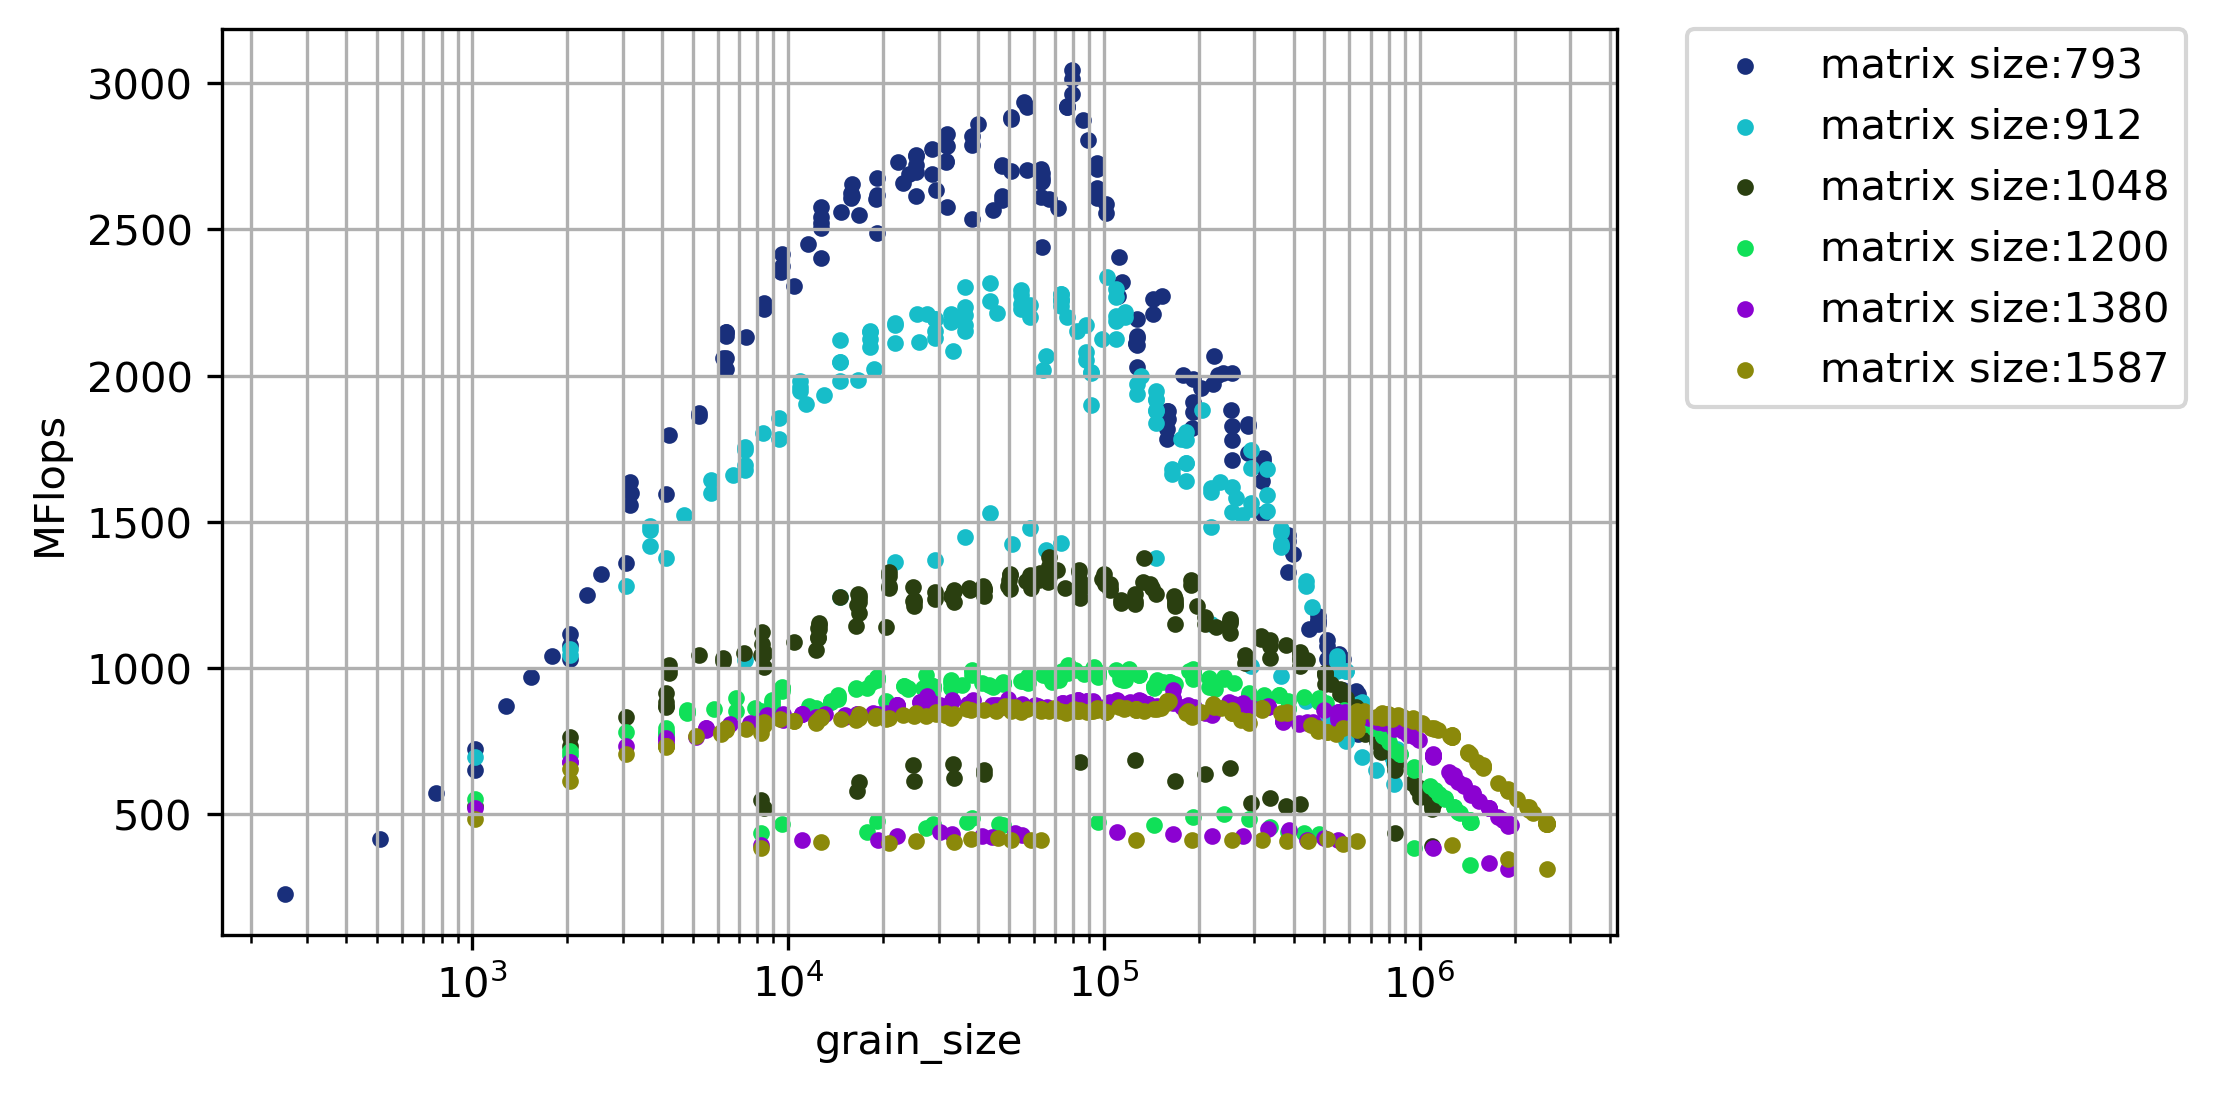
\includegraphics[scale=.75]{images/fig12.png}
	\label{fig8:b}}
	\caption{Throughput vs. grain size graph obtained from running $DMATDMATADD$ benchmark  on $4$ cores for matrix sizes (a) smaller than 793$\times$793 and (b) larger than 793$\times$793.}
	\label{fig8}	
\end{figure}



\vspace{\baselineskip}	
\section{Method}
Looking at the throughput vs. grain size graphs and the consistent pattern observable motivated us to try to model the relationship between throughput and grain size. 
In order to simplify the process and eliminate the effect of different possible factors, we started with limiting the problem to a fixed matrix size. 

\vspace{\baselineskip}	
\subsection{Polynomial Fit}
In our first attempt we used a 2nd degree polynomial to model throughput against grain size. For each matrix size, we fitted the corresponding graphs shown in Figure~\ref{fig8} to a second degree polynomial. 

\begin{figure}[H]
	\centering
	\subfloat[]{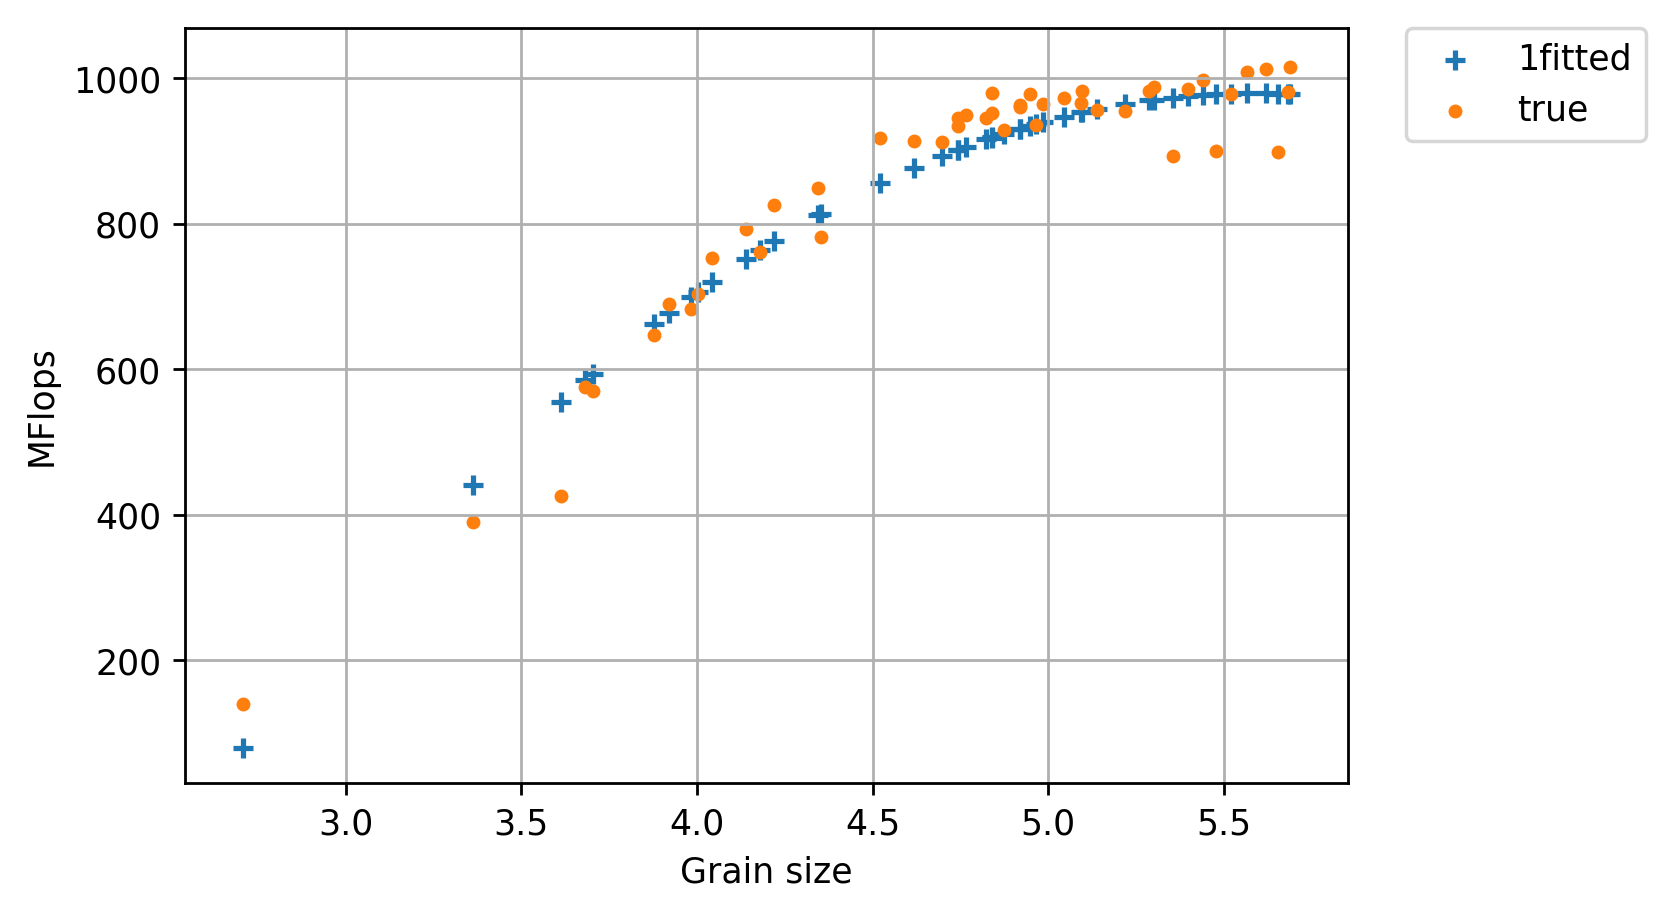
\includegraphics[scale=.45]{images/polyfit/fig_1_690.png}\label{fig10:a}}
	\subfloat[]{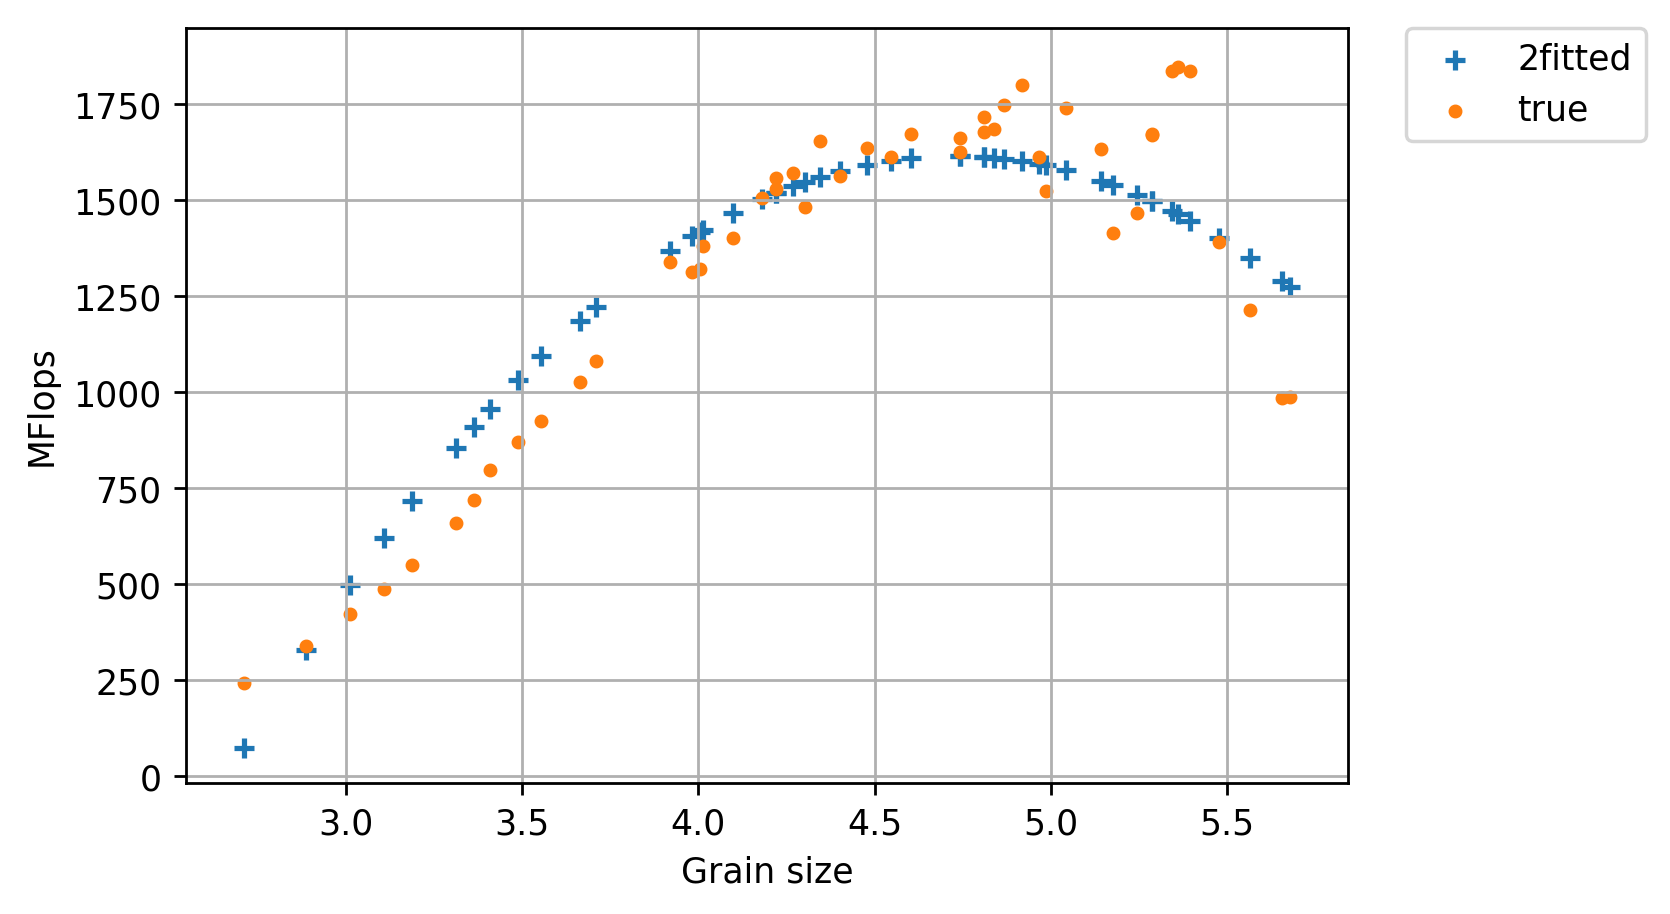
\includegraphics[scale=.45]{images/polyfit/fig_2_690.png}\label{fig10:b}}{\hfill}
	\subfloat[]{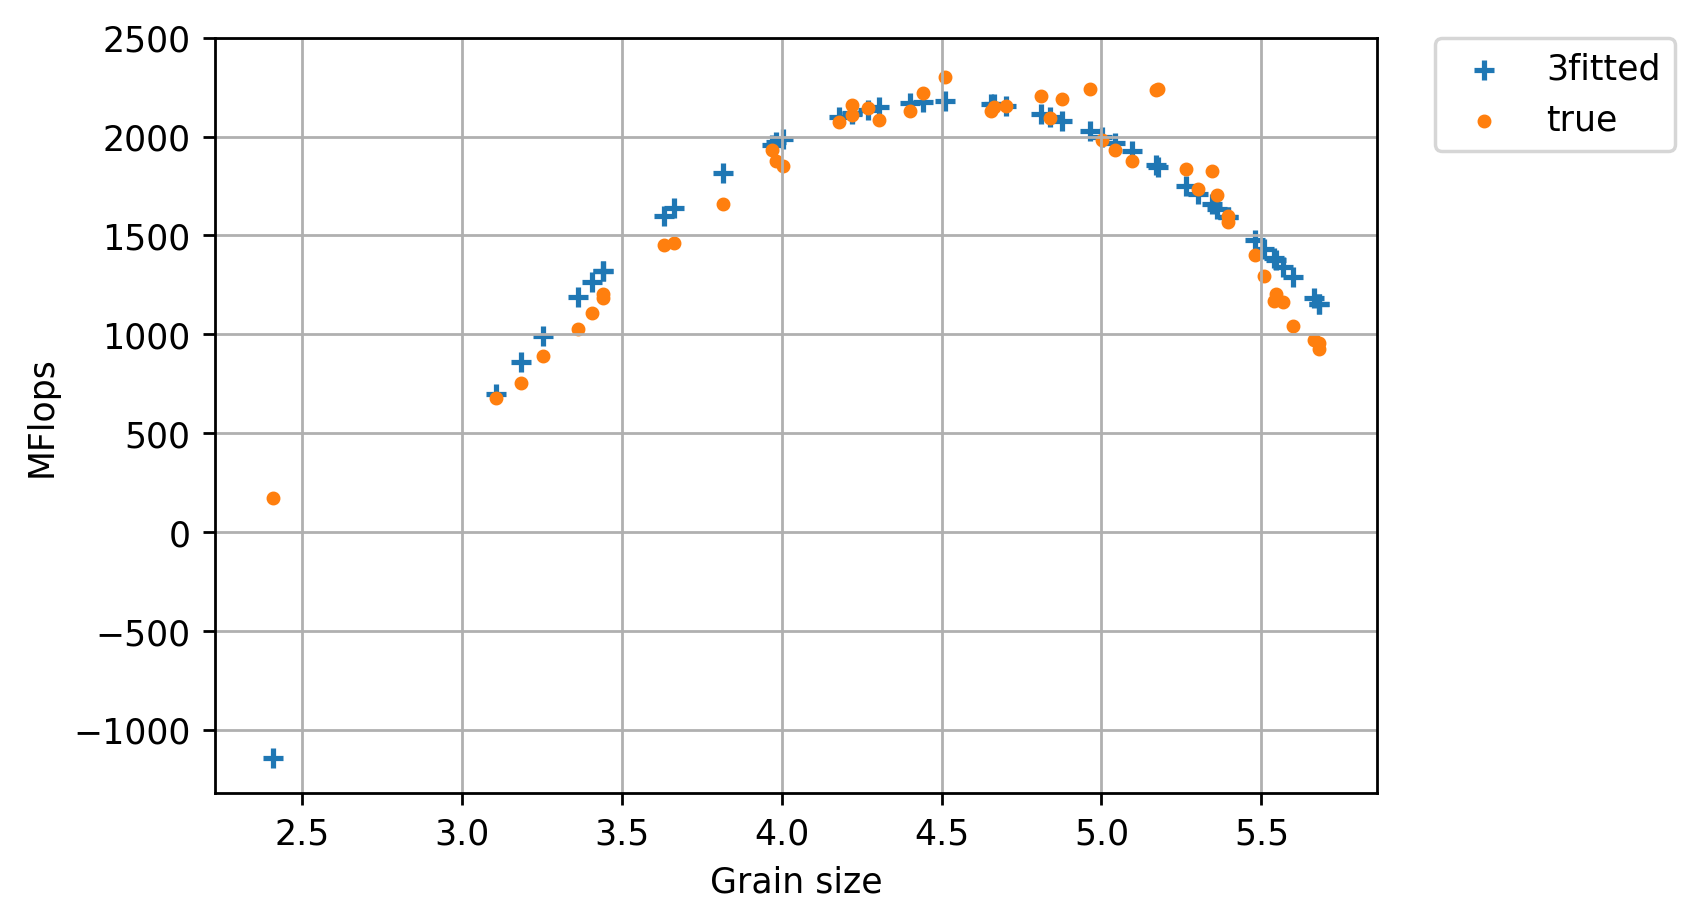
\includegraphics[scale=.45]{images/polyfit/fig_3_690.png}\label{fig10:c}}
	\subfloat[]{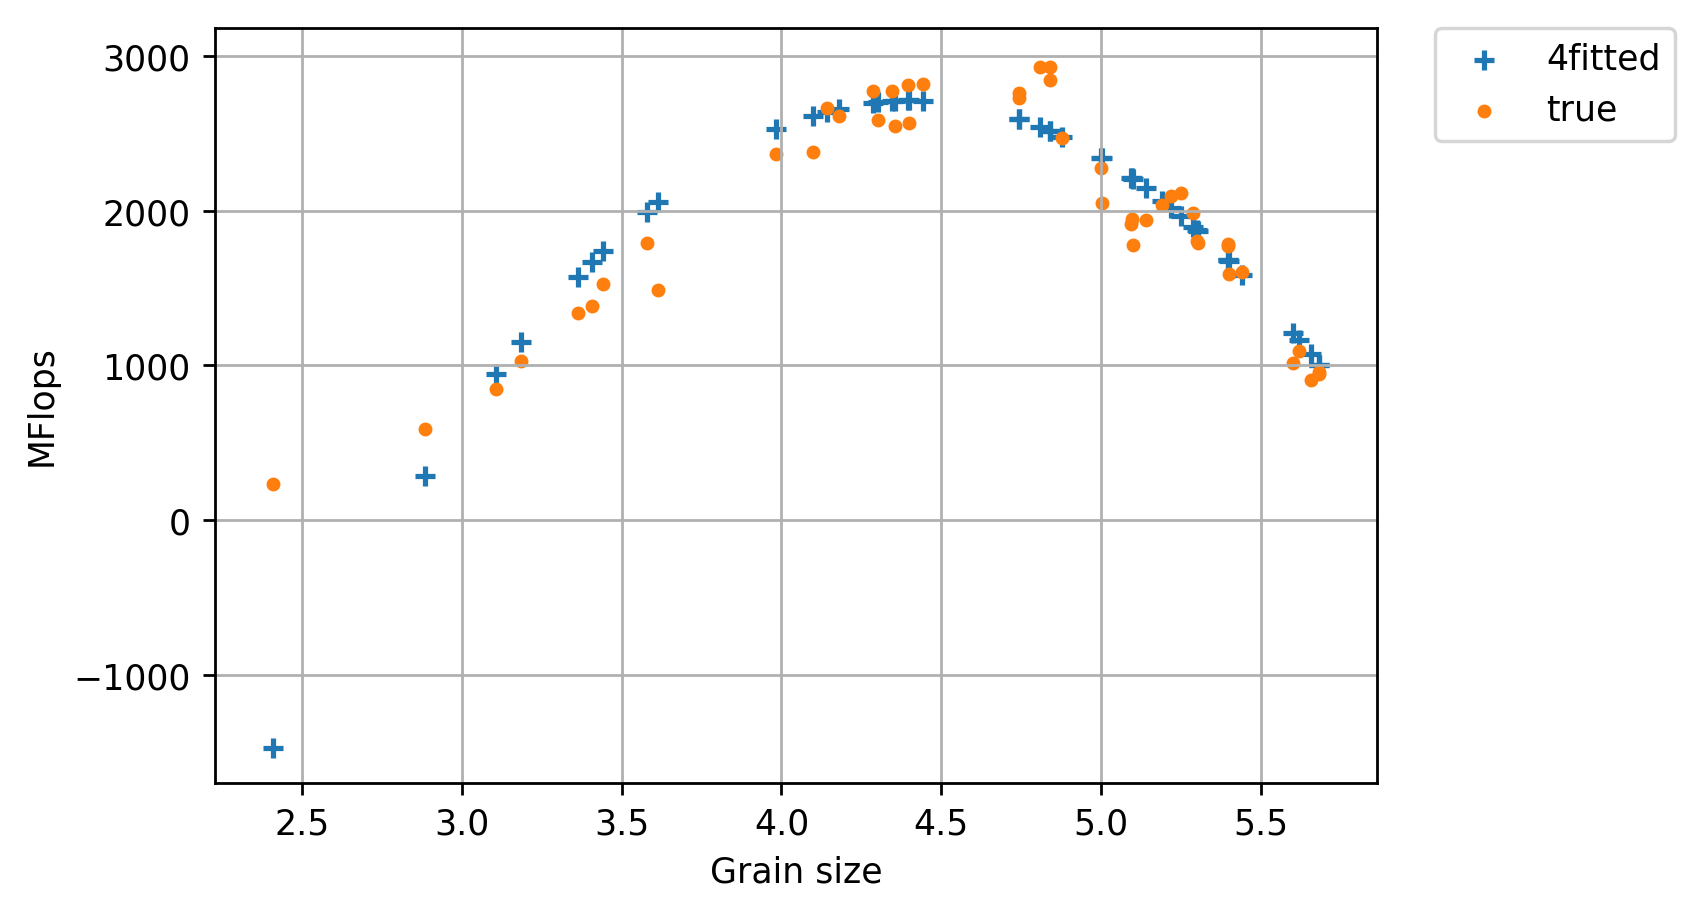
\includegraphics[scale=.45]{images/polyfit/fig_4_690.png}\label{fig10:d}}{\hfill}
	\subfloat[]{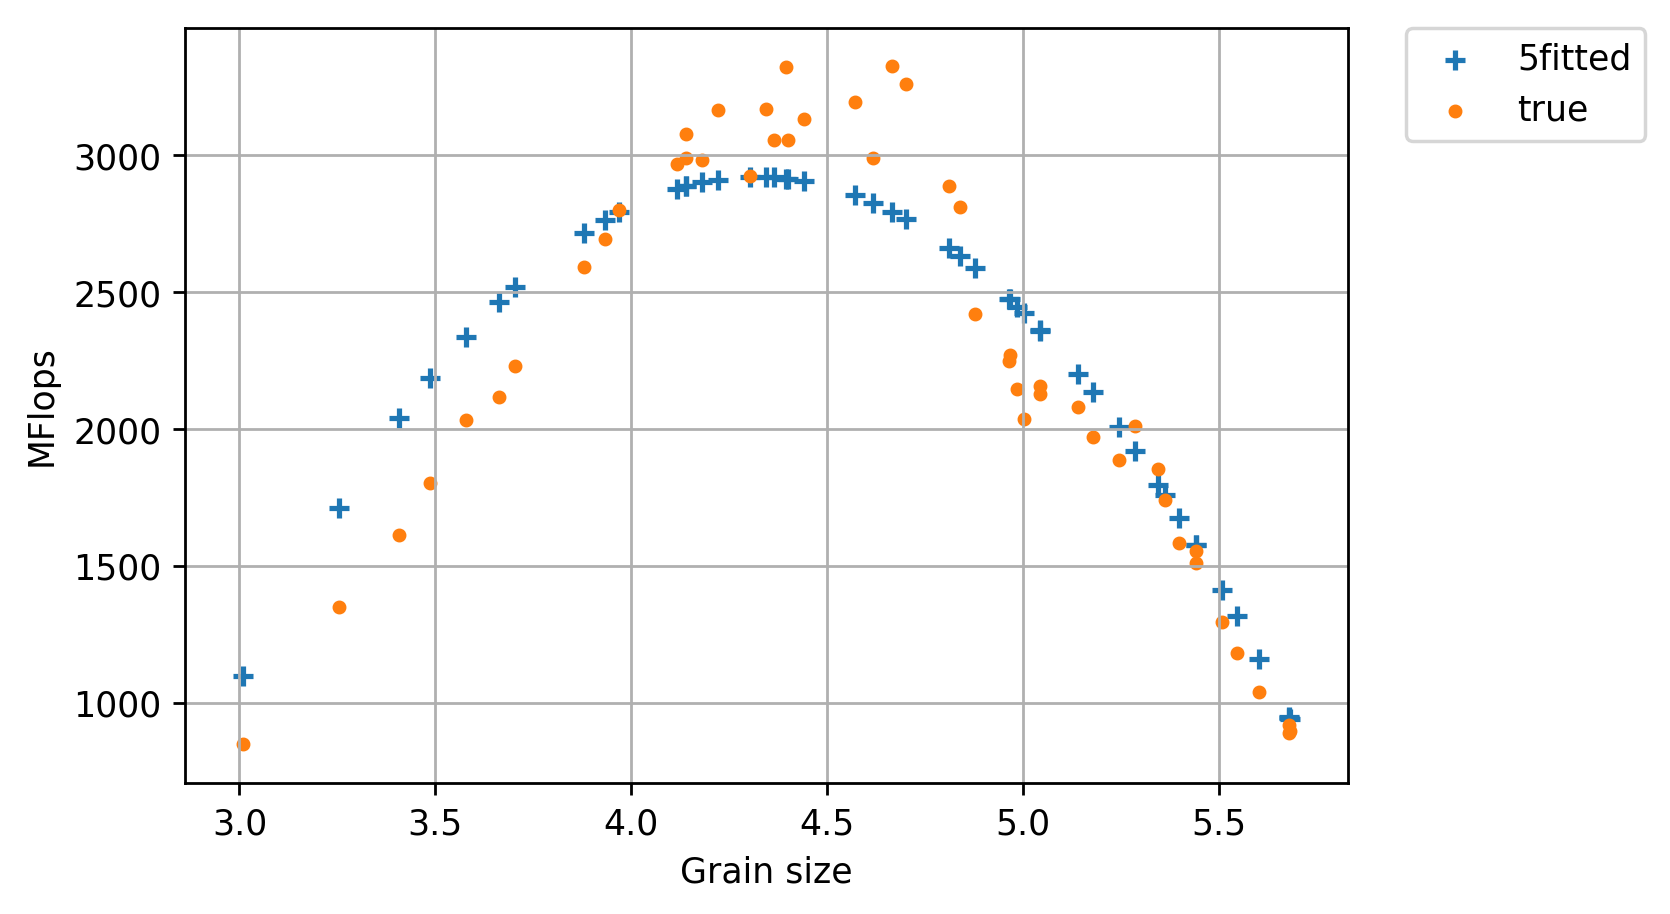
\includegraphics[scale=.45]{images/polyfit/fig_5_690.png}\label{fig10:e}}
	\subfloat[]{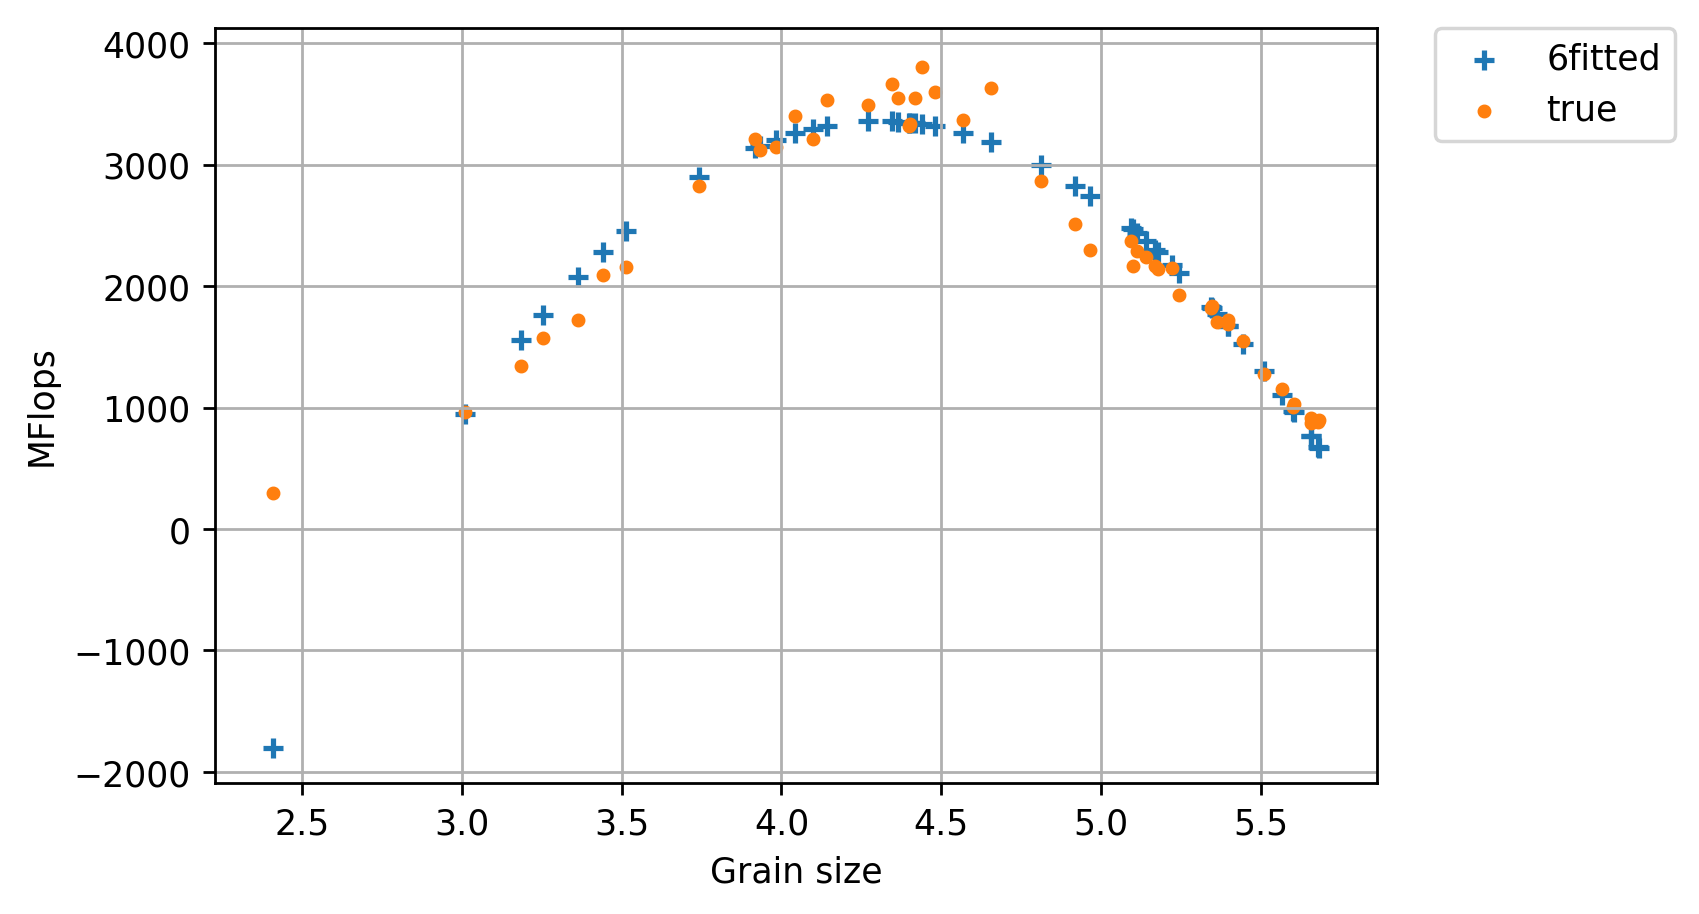
\includegraphics[scale=.45]{images/polyfit/fig_6_690.png}\label{fig10:f}}{\hfill}
	\subfloat[]{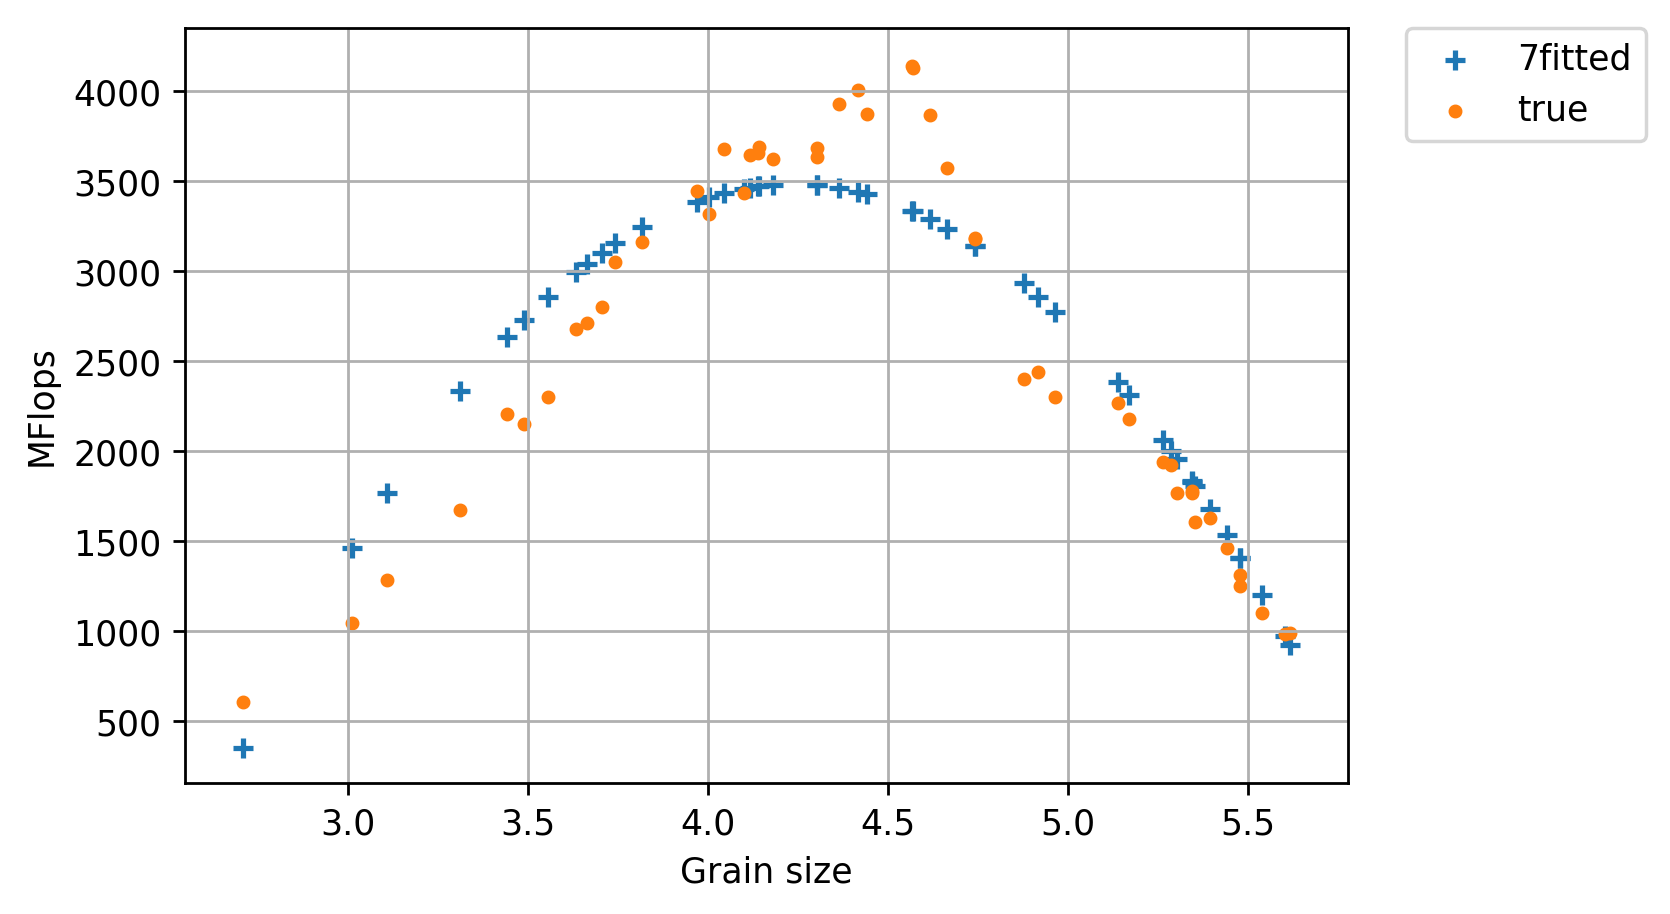
\includegraphics[scale=.45]{images/polyfit/fig_7_690.png}\label{fig10:g}}
	\subfloat[]{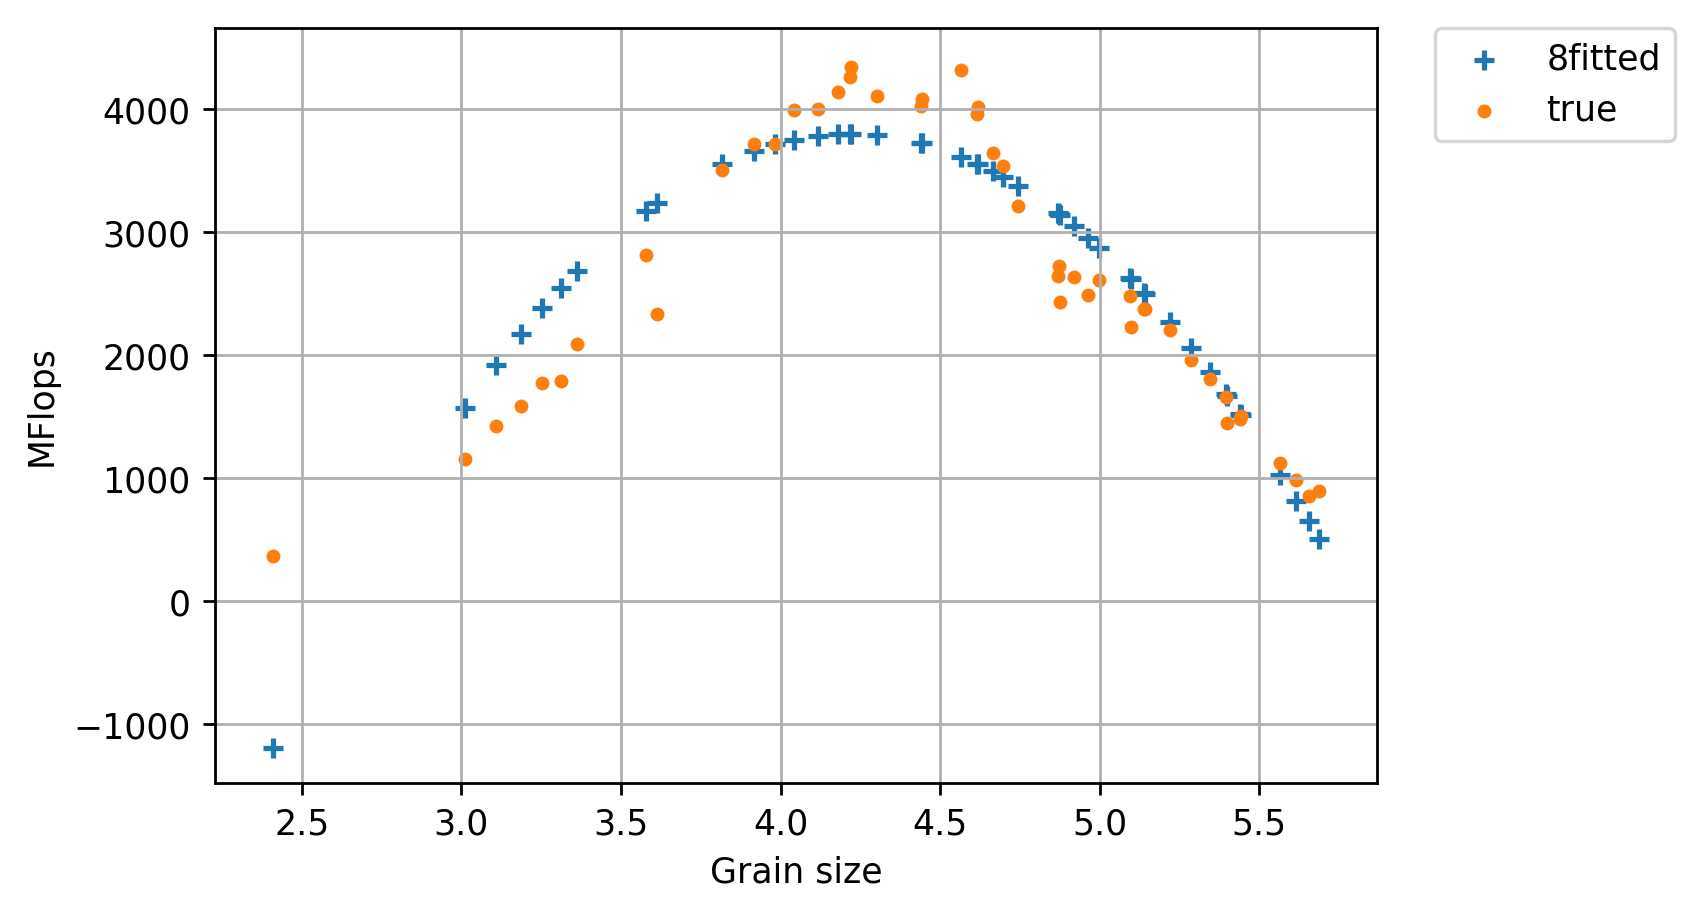
\includegraphics[scale=.45]{images/polyfit/fig_8_690.png}\label{fig10:h}}
							
	\caption{The results of fitting the throughput vs grain size data into a 2d polynomial for $DMATDMATADD$ benchmark for matrix size 690$\times$690 with different number of cores on the test data set (a) 1 core, (b) 2 cores, (c) 3 cores, (d) 4 cores, (e) 5 cores, (f) 6 cores, (g) 7 cores, (h) 8 cores.}	
	\label{fig10}
\end{figure}


\vspace{\baselineskip}	
Figure~\ref{fig10} shows the results of using a quadratic function to fit the data for one matrix size with different number of threads. 

For our experiment, we divided the data into two sections, training and test. $60\%$ of the data was randomly chosen for the training part and the rest was considered as the test set. The training set was used to find the best 2nd degree polynomial for the data, and once the parameters were identified, the generated 2nd degree polynomial was applied to the test set to measure how good our fit was performing. 

For the matrix size $690\times690$ our dataset contained 117 data points, 72 of which was randomly selected to build the model. The mean relative error for each number of cores, calculated using Equation~\ref{eq2}, is represented in Figure~\ref{fig11} for training and test set. In this equation, $t_i$ and $p_i$ denote the true value and the predicted value of the $i$th sample respectively, where $n$ is the number of samples with the particular number of cores. 

\begin{equation}{\label{eq2}}
Relative\,\,Error = \frac{1}{n}\sum_{i=1}^{n} {1-p_i/t_i}
\end{equation}

\vspace{\baselineskip}	
\begin{figure}[H]
	\centering
	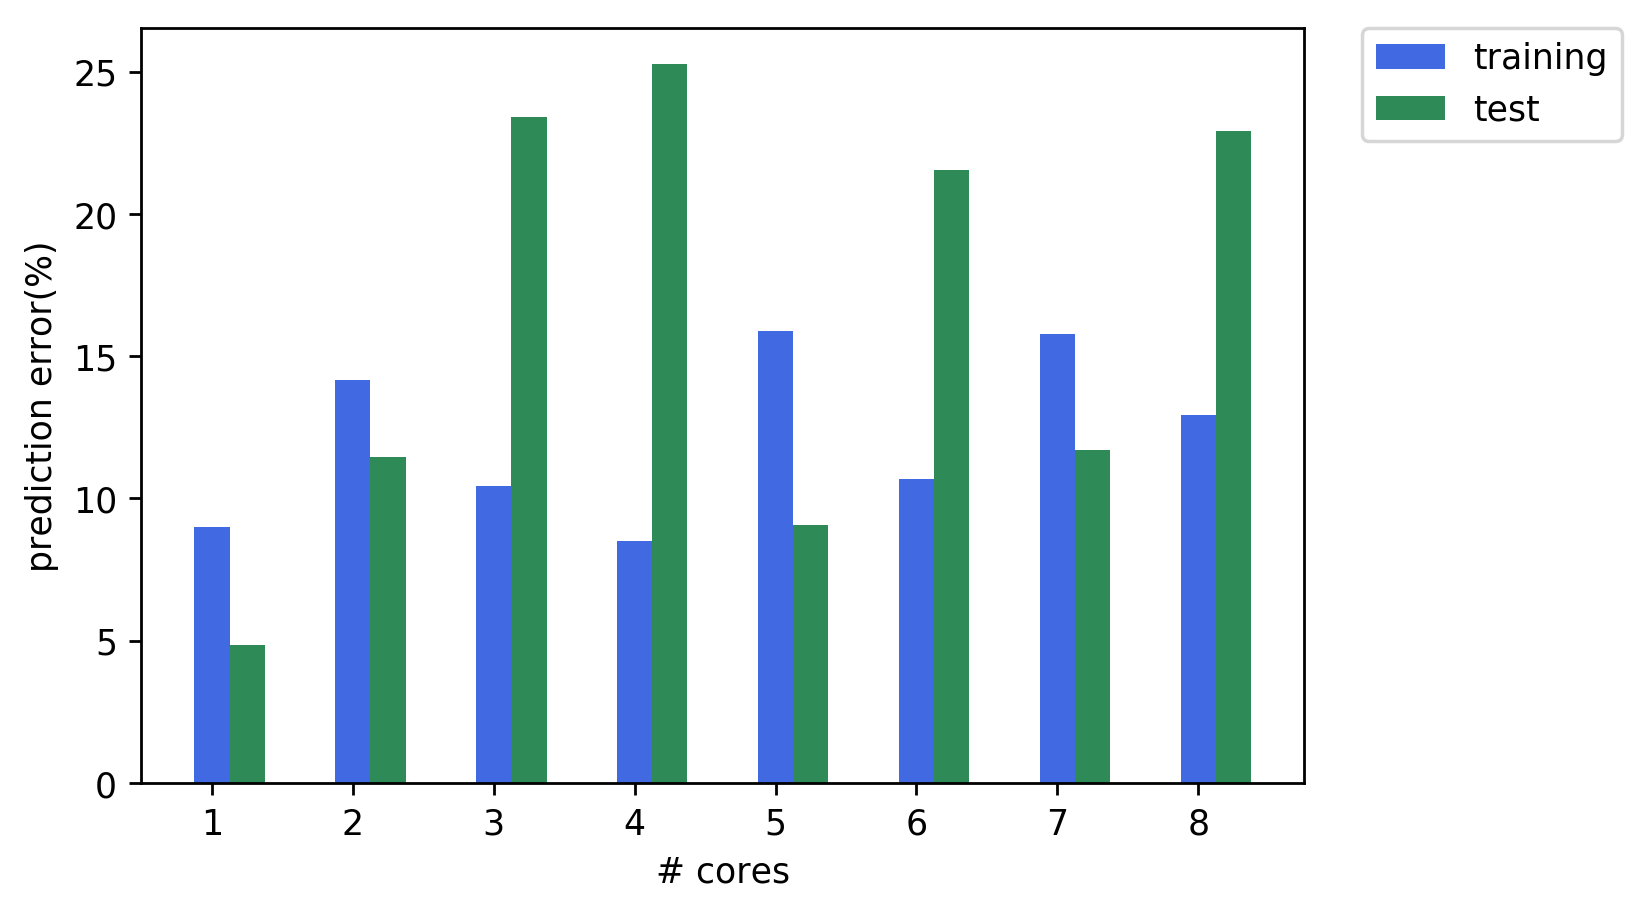
\includegraphics[scale=.75]{images/polyfit/fig_train_test_690.png}
	\caption{The training and test error for fitting data obtained from the $DMATDMATADD$ benchmark for matrix size $690\times690$ against different number of cores cores.}	
	\label{fig11}
\end{figure}

\vspace{\baselineskip}	
\subsubsection{Generalizing the fitted function to include number of cores}
In this step, we try to generalize the fitted 2nd degree polynomial obtained from the previous step, represented by $P=ag^2+bg+c$, where $P$ is the throughput and $g$ is the grain size,by looking at how the three parameters $a$, $b$, and $c$ change when number of cores changes. 
A $3$rd degree polynomial seems to a reasonable fit for each of these parameters, in regards to number of cores. In order to avoid overfitting, we excluded two of the data points($2$ and $5$) from the data points used for fitting the polynomial and tested the fitted function on those two points to see how well the function is working on unseen data points. 


\vspace{\baselineskip}	
\begin{figure}[H]
	\centering
	\subfloat[]{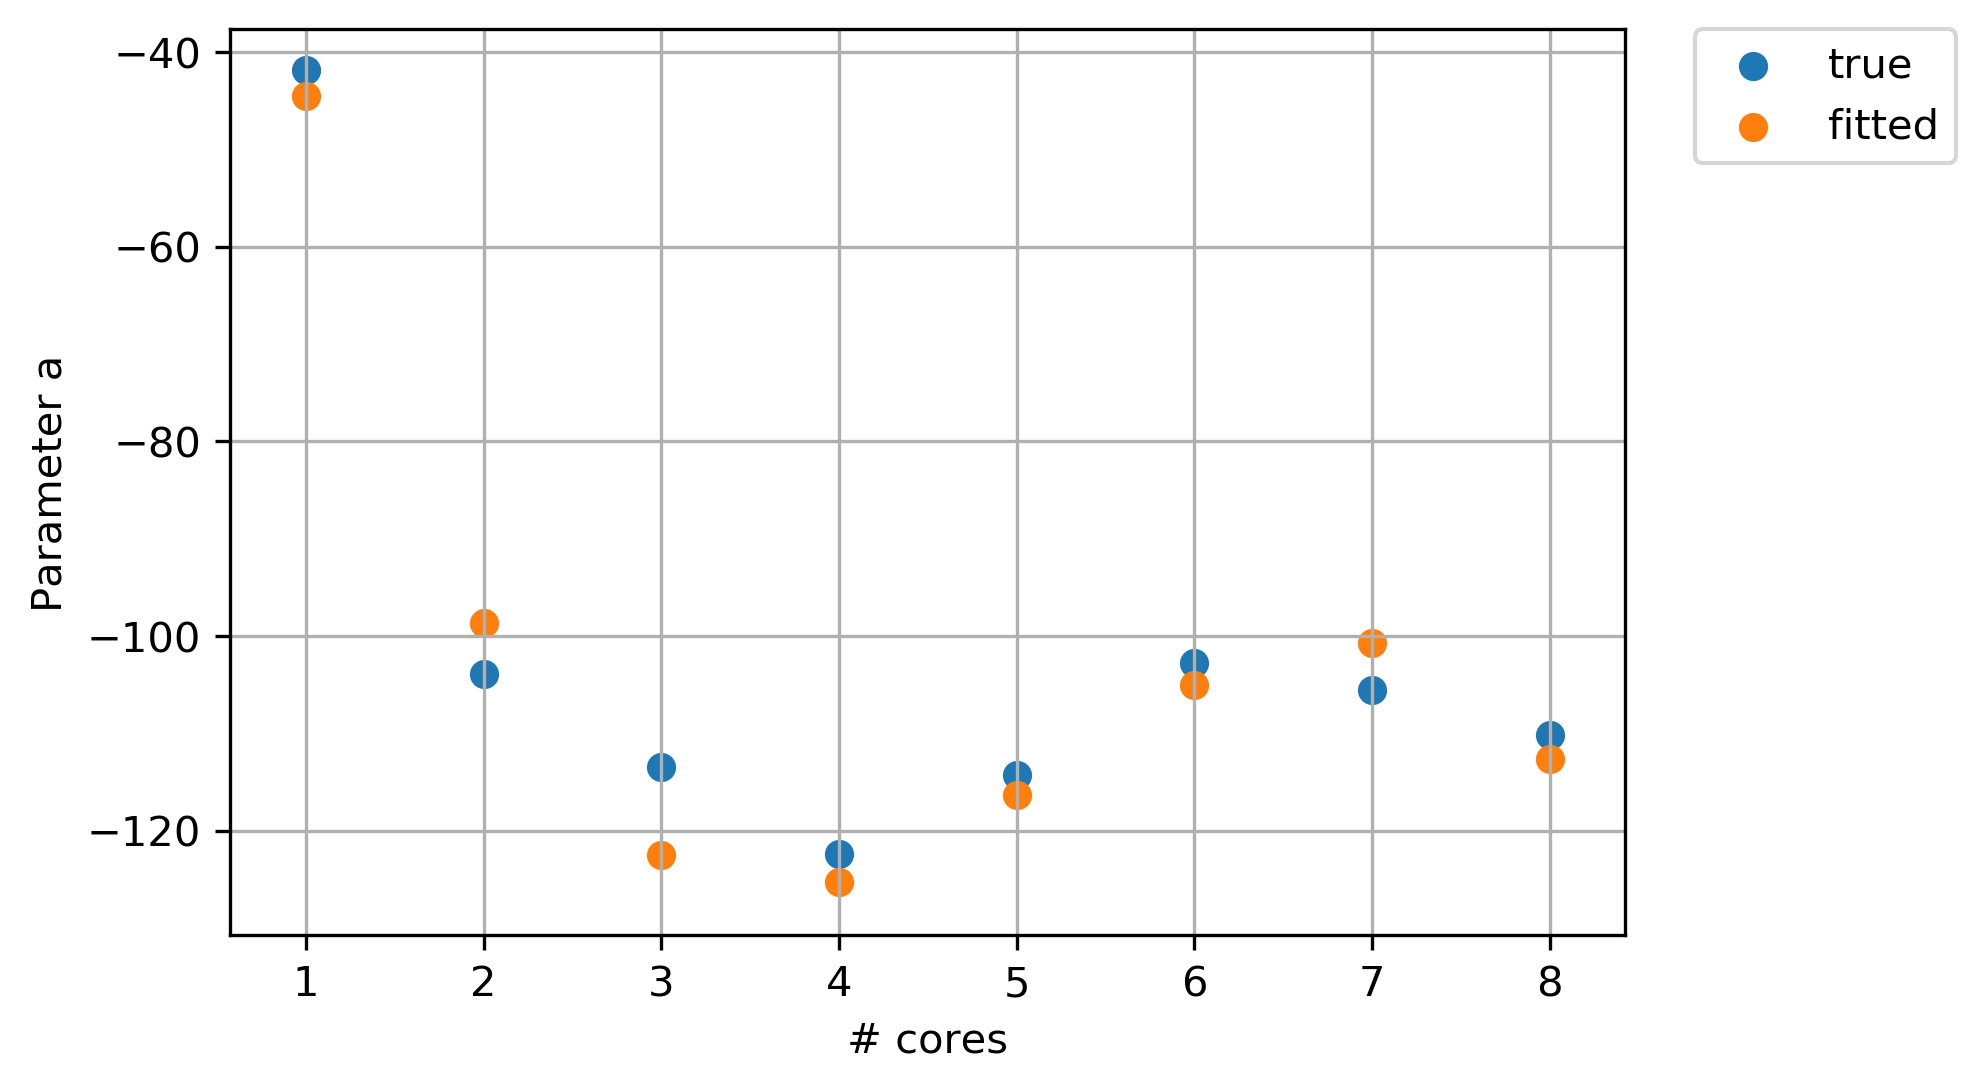
\includegraphics[scale=.3]{images/polyfit/fig_690_params_0.png}\label{fig15:a}}
	\subfloat[]{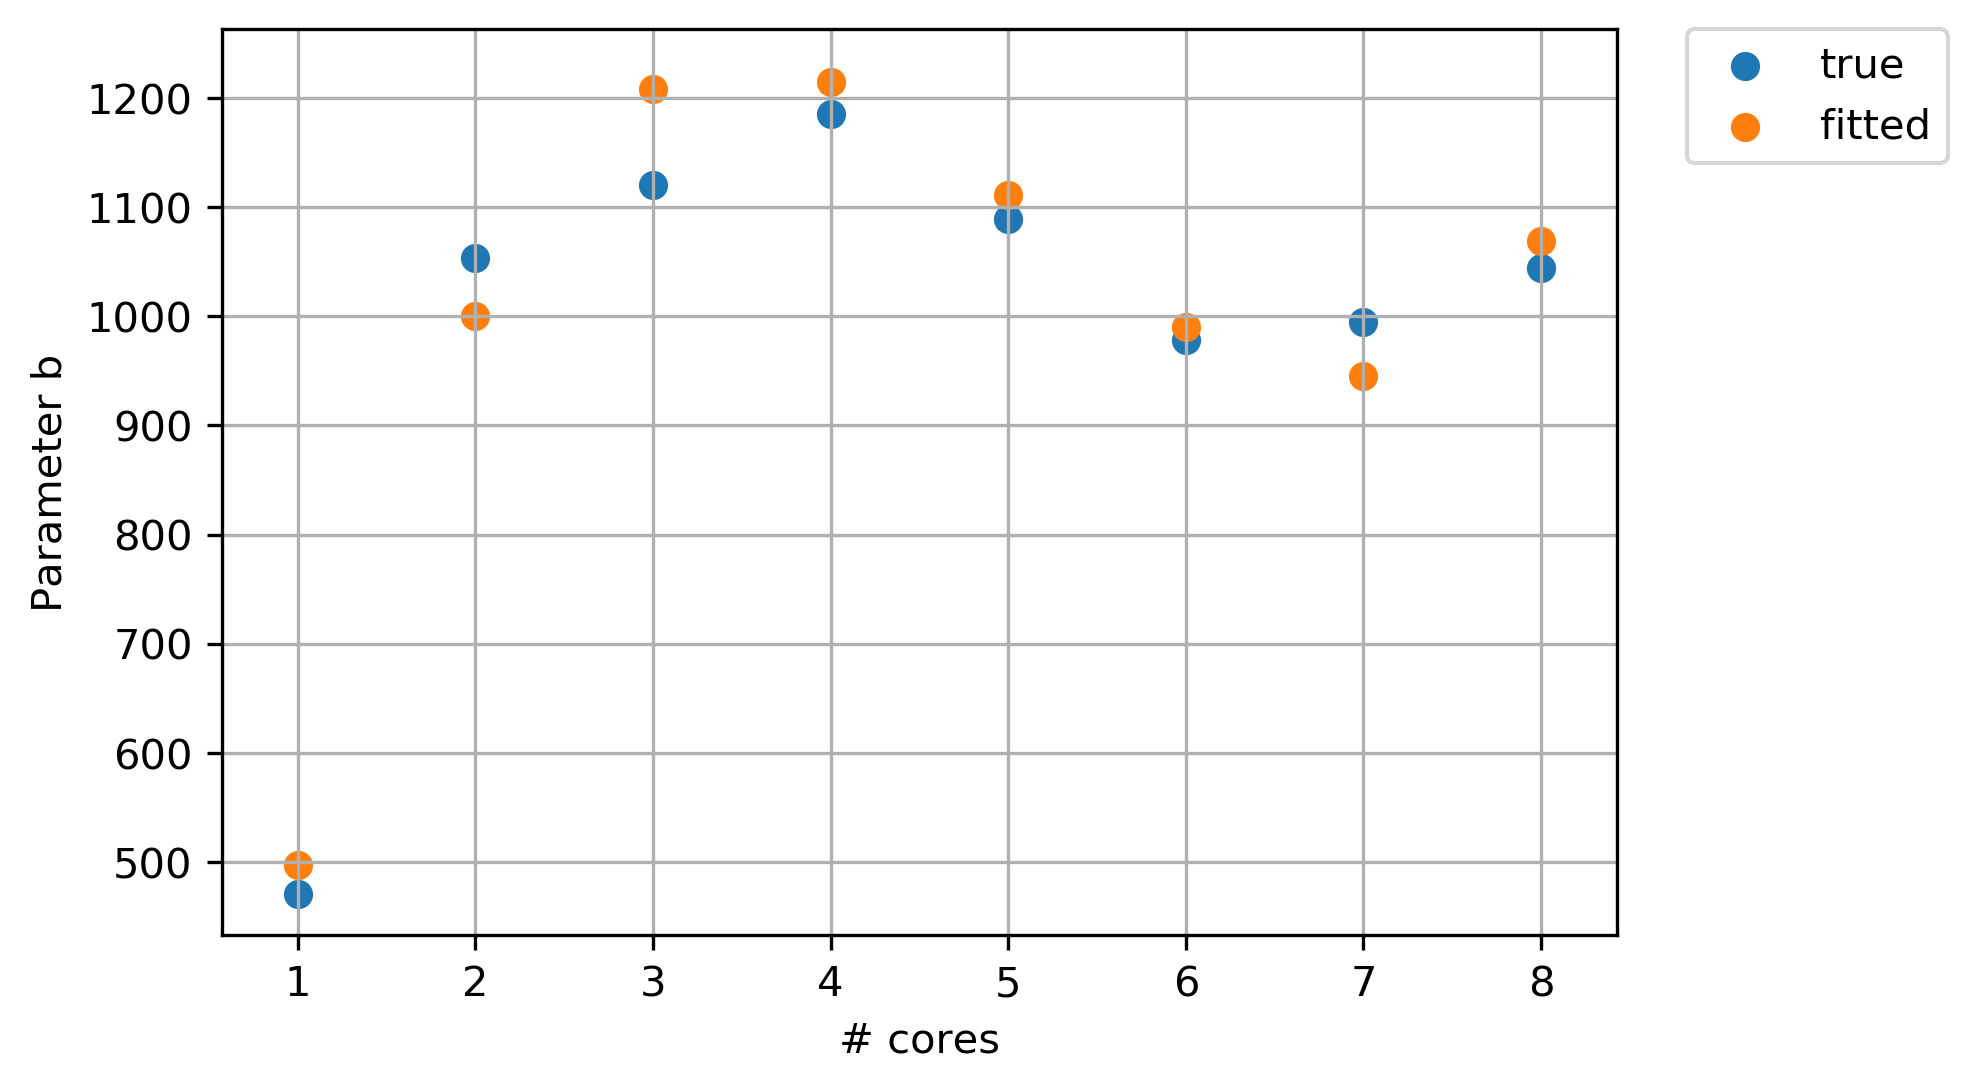
\includegraphics[scale=.3]{images/polyfit/fig_690_params_1.png}\label{fig15:b}}
	\subfloat[]{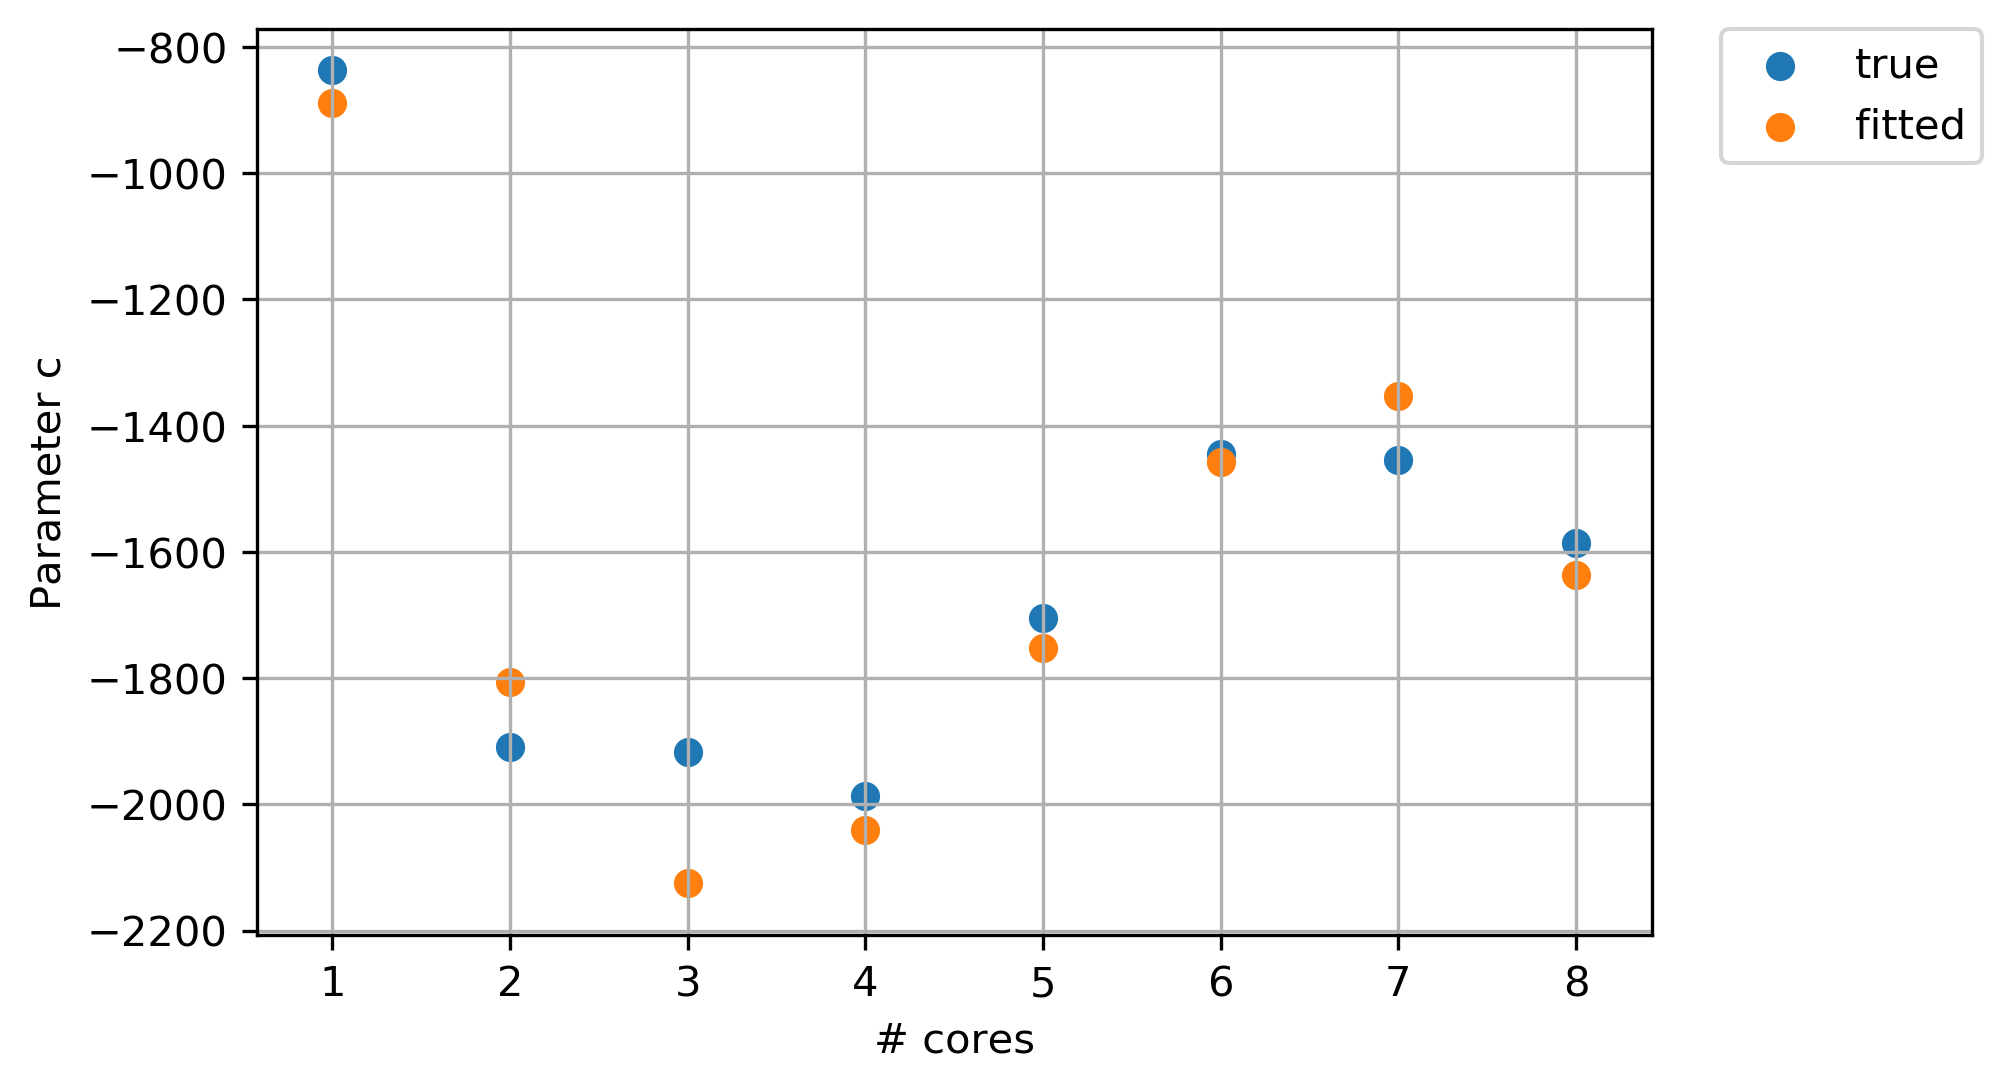
\includegraphics[scale=.3]{images/polyfit/fig_690_params_2.png}\label{fig15:c}}
	\caption{Fitting the parameters of the quadratic function with a $3$rd degree polynomial from the $DMATDMATADD$ benchmark for matrix size $690\times690$ against different number of cores.}	
	\label{fig15}
\end{figure}

\vspace{\baselineskip}	
\begin{figure}[H]
	\centering
	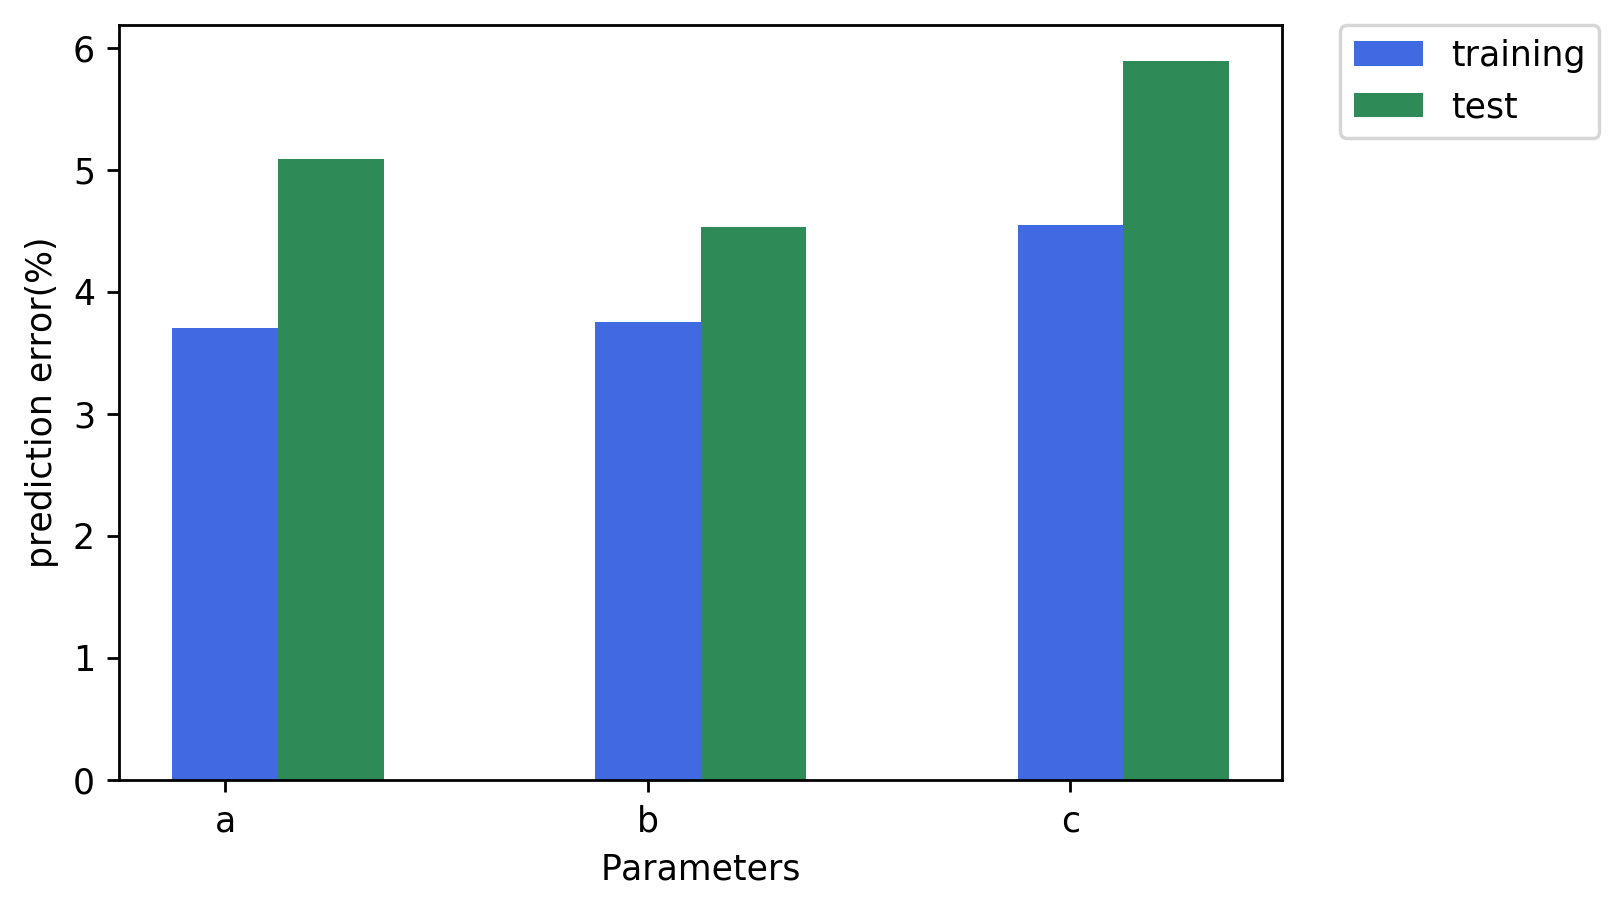
\includegraphics[scale=.45]{images/polyfit/fig_690_params_error.png}
	
	\caption{The error in fitting the parameters $a$, $b$, and $c$ for matrix size $690\times690$.}	
	\label{fig16}
\end{figure}

Using this $3$rd degree polynomial to fit the parameters, we can generalize the relationship between throughput and grain size in the following equation:

\begin{equation}\label{eq3}
P=a_{11}g^2N^3+a_{10}g^2N^2+...+a_1N+a_0
\end{equation}
where $P$ is the throughput, $g$ is the grain size, and $N$ is the number of cores and coefficients $a_{11},...,a_0$ are the real values.

Knowing that a polynomial of degree $2$ in terms of grain size and of degree $3$ in terms of number of cores, we can try to fit our original data directly to the above mentioned formula (Equation~\ref{eq3}). The results of the original data obtained from running $DMATDMATADD$ benchmark, the fitted polynomial based on Equation~\ref{eq3}, is represented in Figure~\ref{fig18}, for 2,4, and 8 cores for a matrix of size $690\times690$.

\vspace{\baselineskip}	
\begin{figure}[H]
	\centering
	\subfloat[]{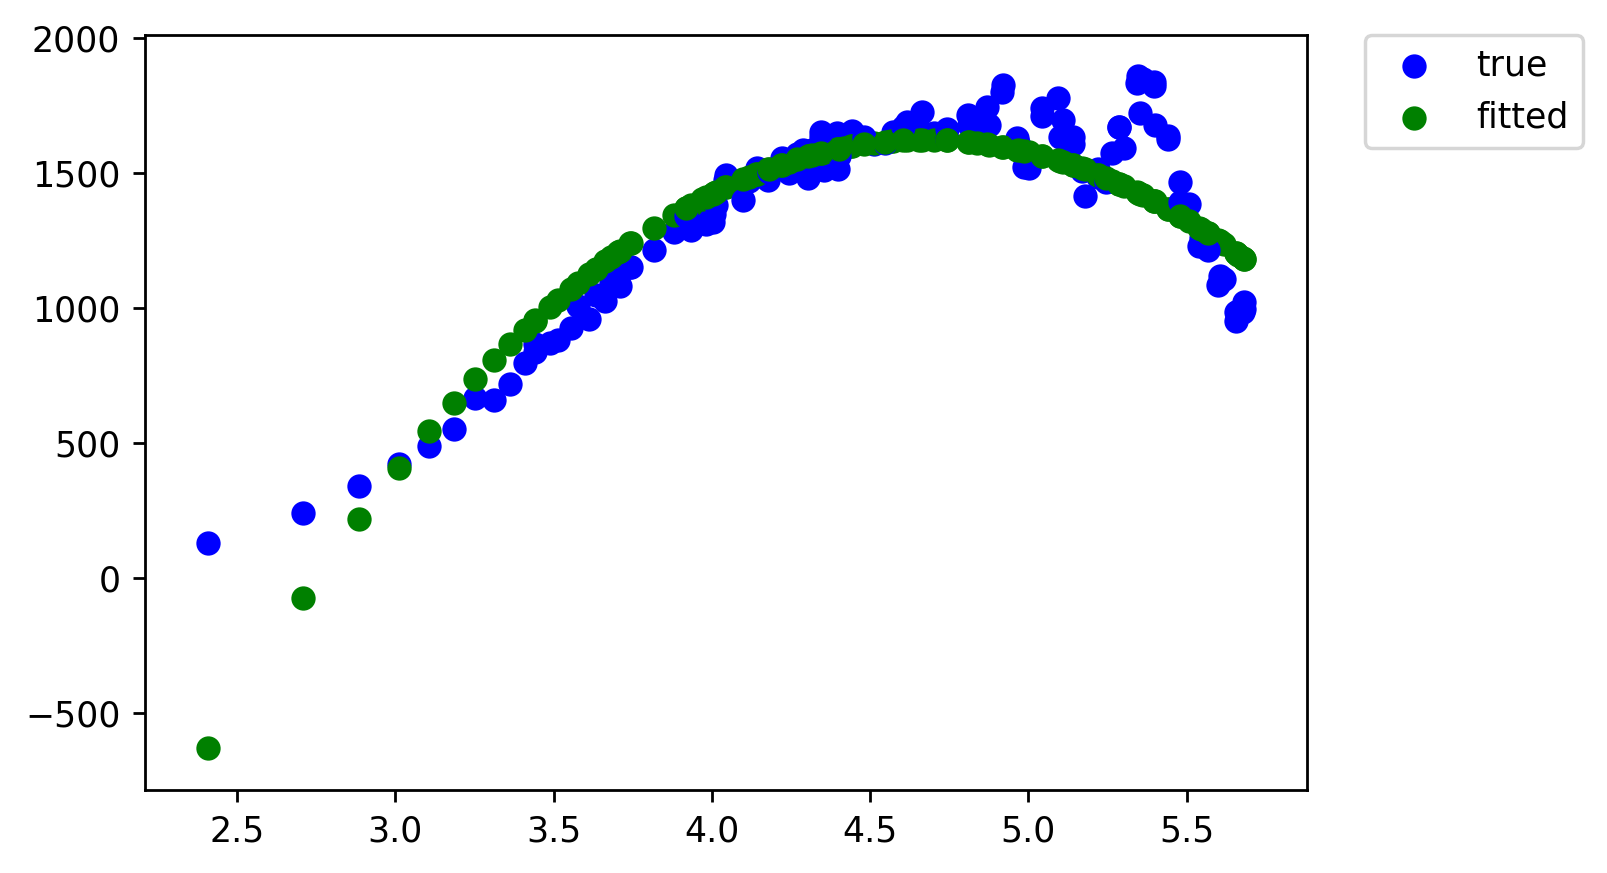
\includegraphics[scale=.35]{images/polyfit/fig_690_total_2.png}\label{fig18:a}}
	\subfloat[]{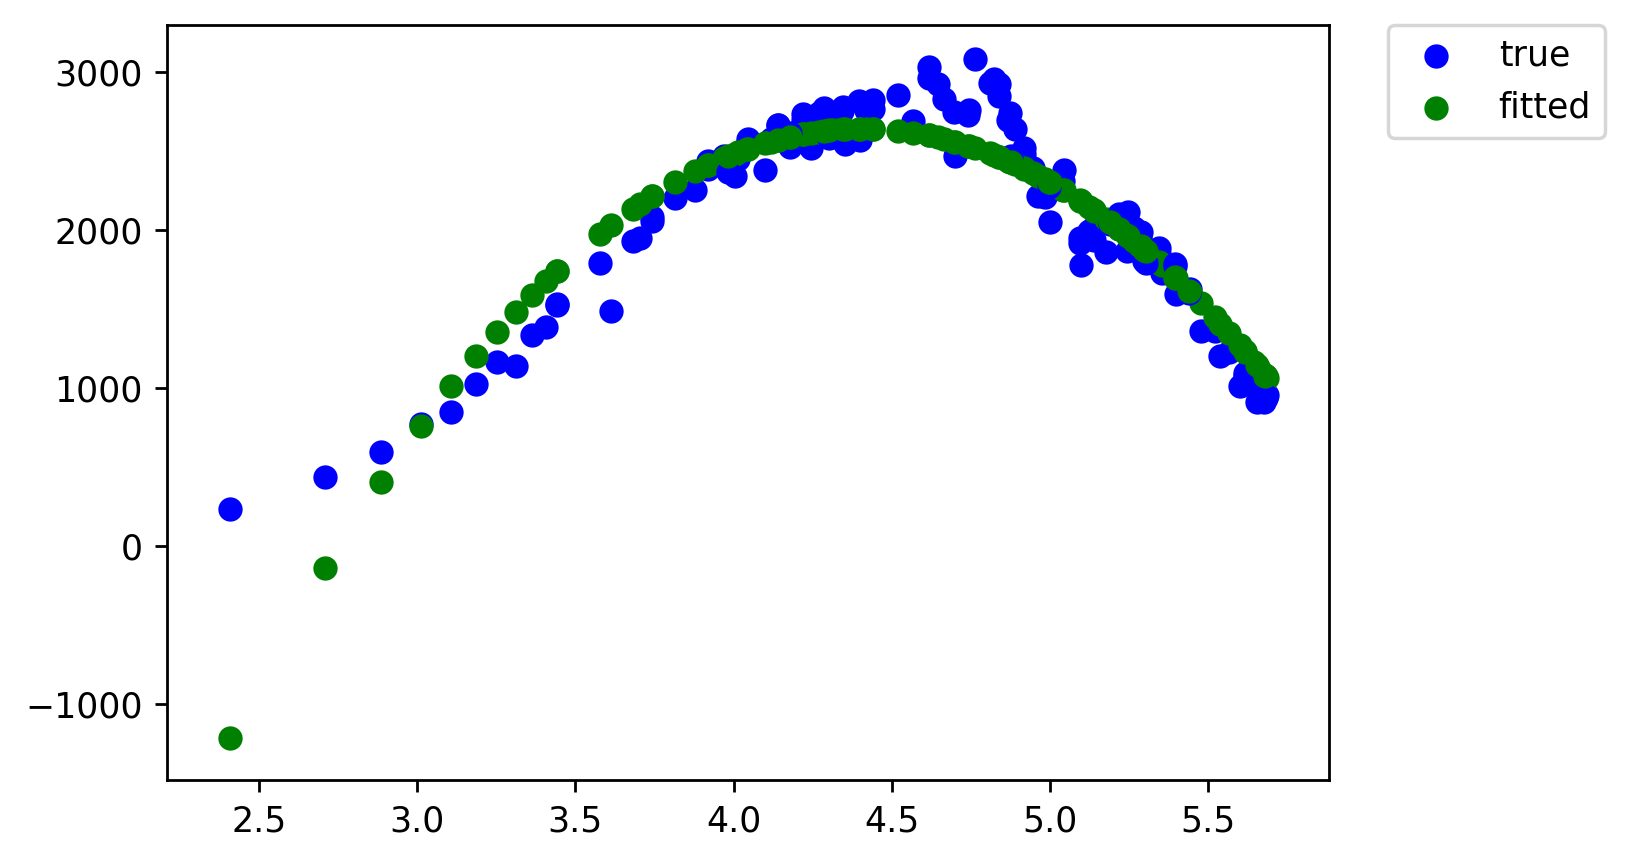
\includegraphics[scale=.35]{images/polyfit/fig_690_total_4.png}\label{fig18:b}}
	\subfloat[]{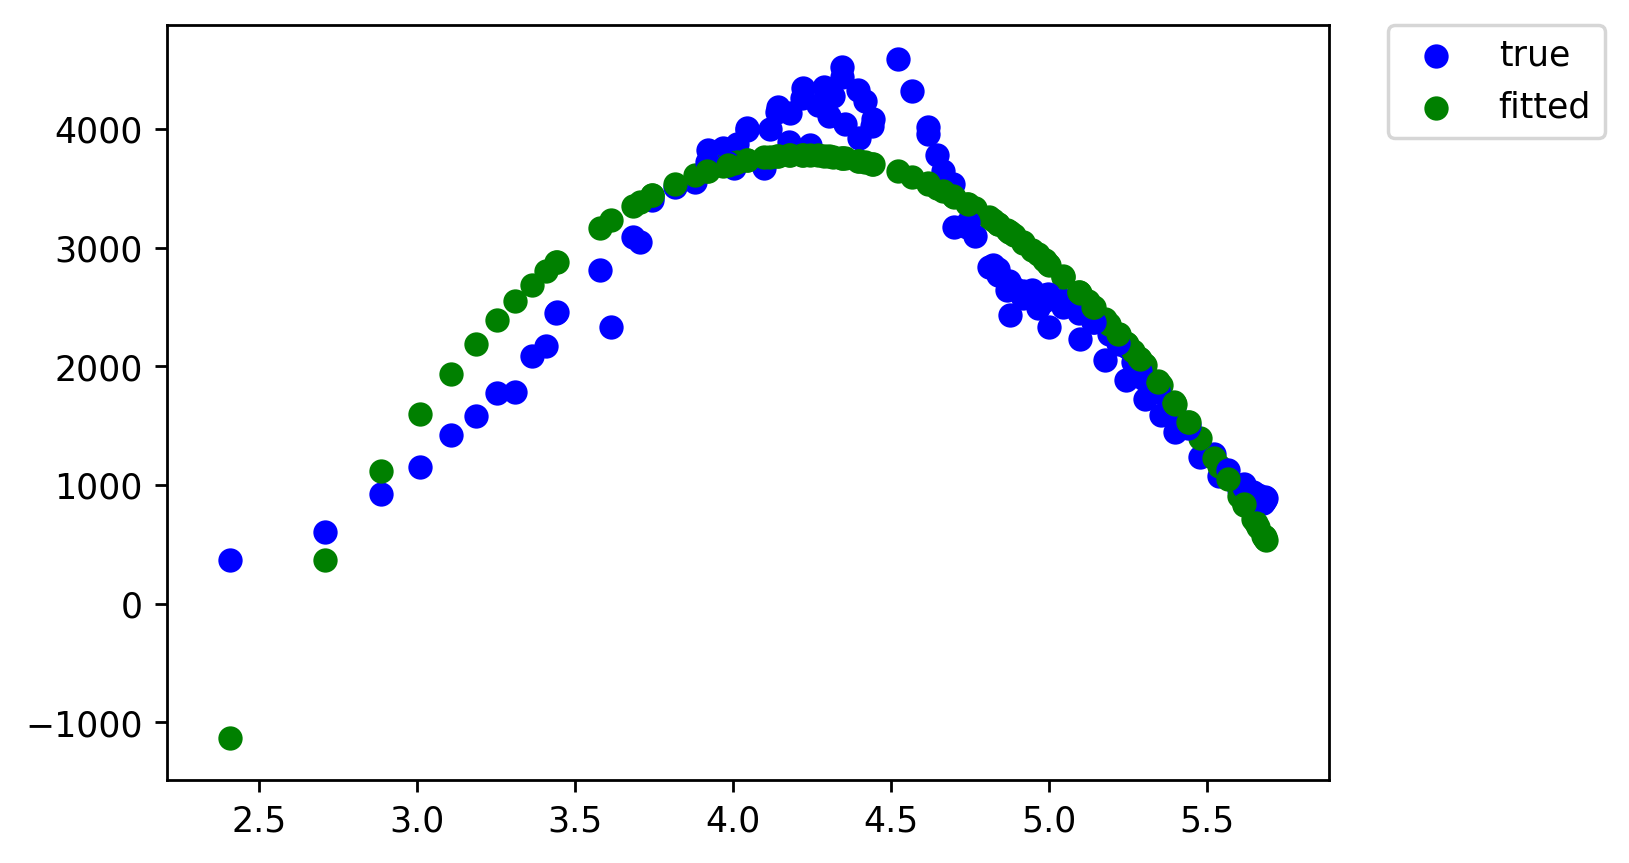
\includegraphics[scale=.35]{images/polyfit/fig_690_total_8.png}\label{fig18:c}}
	\caption{Results of fitting the data from $DMATDMATADD$ benchmark with a polynomial of degree $2$ in terms of grain size and of degree $3$ in terms of number of cores for matrix size $690\times690$ for (a) 2 core, (b) 4 cores, (c) 8 cores.}	
	\label{fig18}
\end{figure}

\vspace{\baselineskip}	
\begin{figure}[H]
	\centering
	\subfloat[]{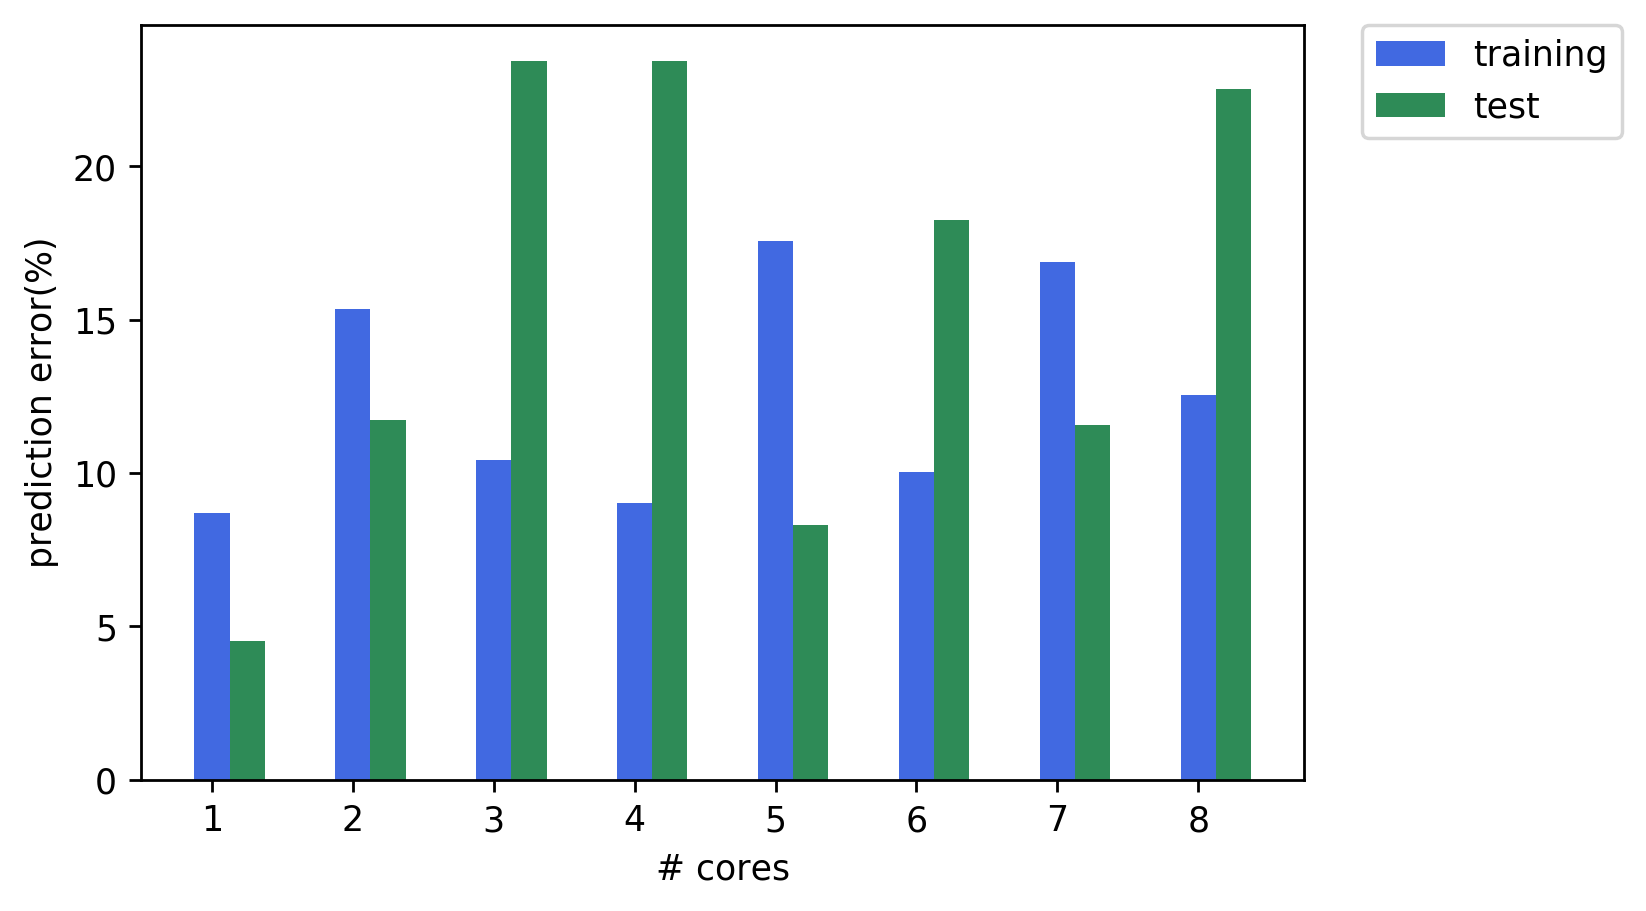
\includegraphics[scale=.45]{images/polyfit/fig_690_total_error.png}\label{fig17:a}}
	\subfloat[]{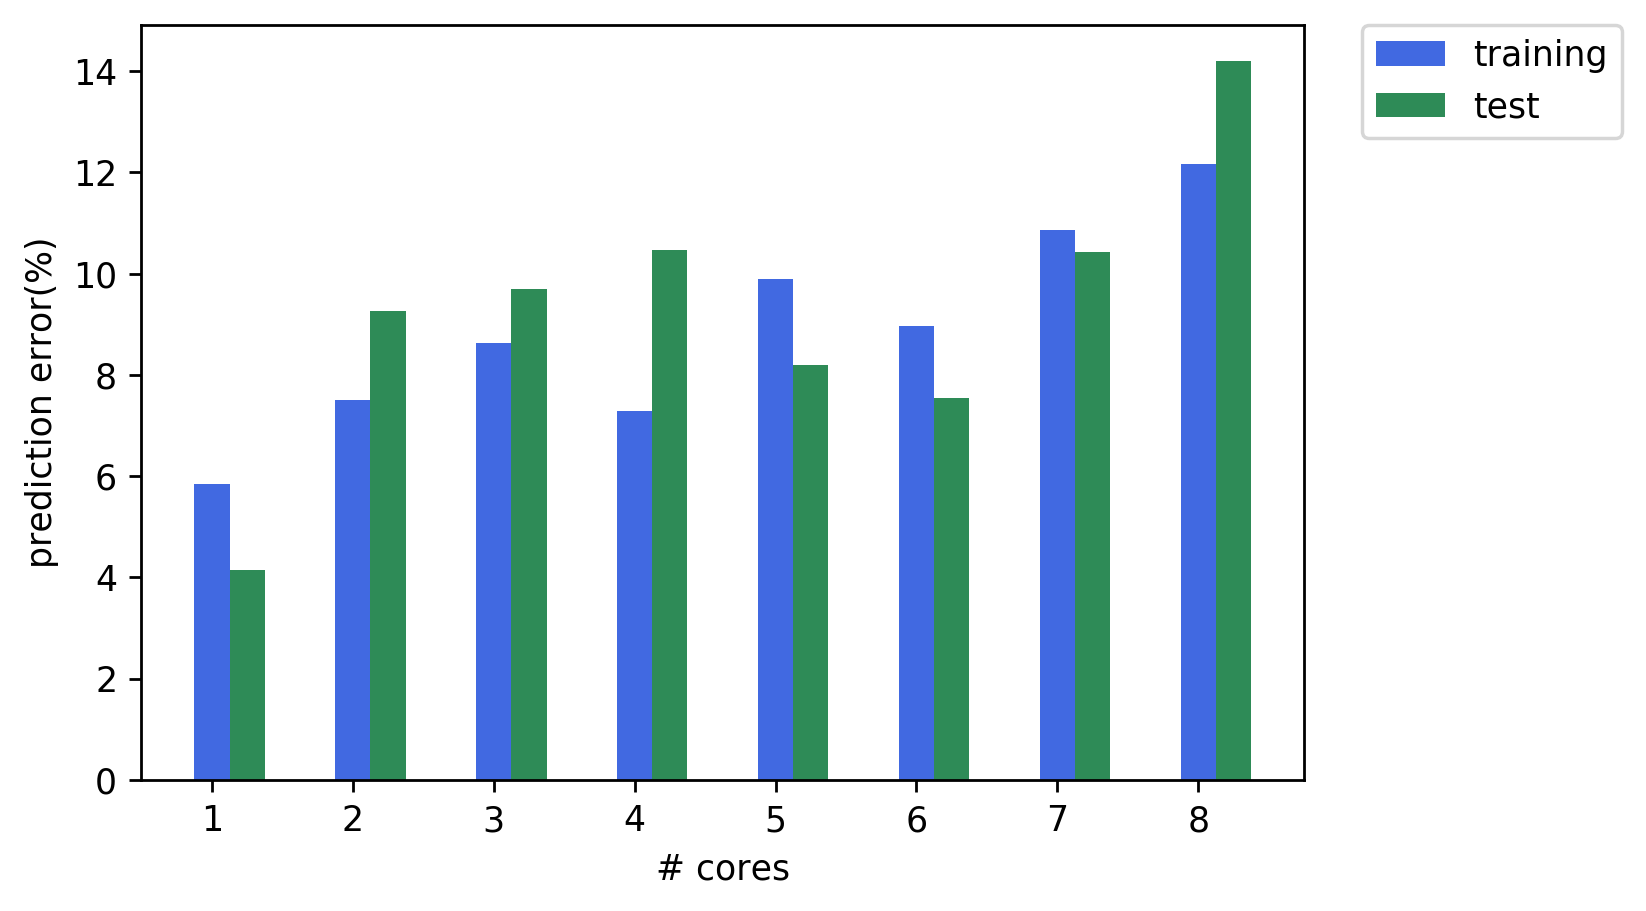
\includegraphics[scale=.45]{images/polyfit/fig_690_total_error_corrected.png}\label{fig17:b}}
	\caption{The training and test error obtained fitting the data to a polynomial of degree $2$ in terms of grain size and of degree $3$ in terms of number of cores for matrix size $690\times690$, for each number of cores. (a) All the data points are include in caluculation of error, (b) the leftmost sample was removed from error calculation.}	
	\label{fig17}
\end{figure}

Figure~\ref{fig17:a} shows the obtained relative error on both training and test sets. The graph suggests a higher test error compared to the training error, mostly caused by the left hand side of the graph. The effect of removing the leftmost sample from error calculations is depicted in Figure~\ref{fig17:b}.

Although we are interested in finding a model that results in a low training and test error, our purpose is mainly finding the region that generates the highest performance. So, even though our model might not match the original data in all data points, due to having a different nature than a quadratic function, our focus would be on how this fit can help us to find which range of grain sizes, or how big the task sizes should be, to achieve the highest performance. 



\vspace{\baselineskip}	
\subsubsection{Finding the range of grain size to achieve the highest performance}
The major advantage of using a quadratic function to fit the data in terms of grain size, when number of cores is fixed, is the simplicity of the formula, which makes it possible for us to find the peak of the graph very easily. n order to add some uncertainty to our prediction, instead of finding the maximum of the quadratic function, we identified the range of grain size that results in a performance within $10\%$ of the maximum performance. For a second degree polynomial in terms of $g$, $P=ag^2+bg+c$, the minimum or maximum of the polynomial is located at $p^{*}=\frac{-b}{2a}$, and $a$, $b$, $c$ are 3rd degree polynomials of number of cores.    

\vspace{\baselineskip}	
\begin{figure}[H]
	\centering
	\subfloat[]{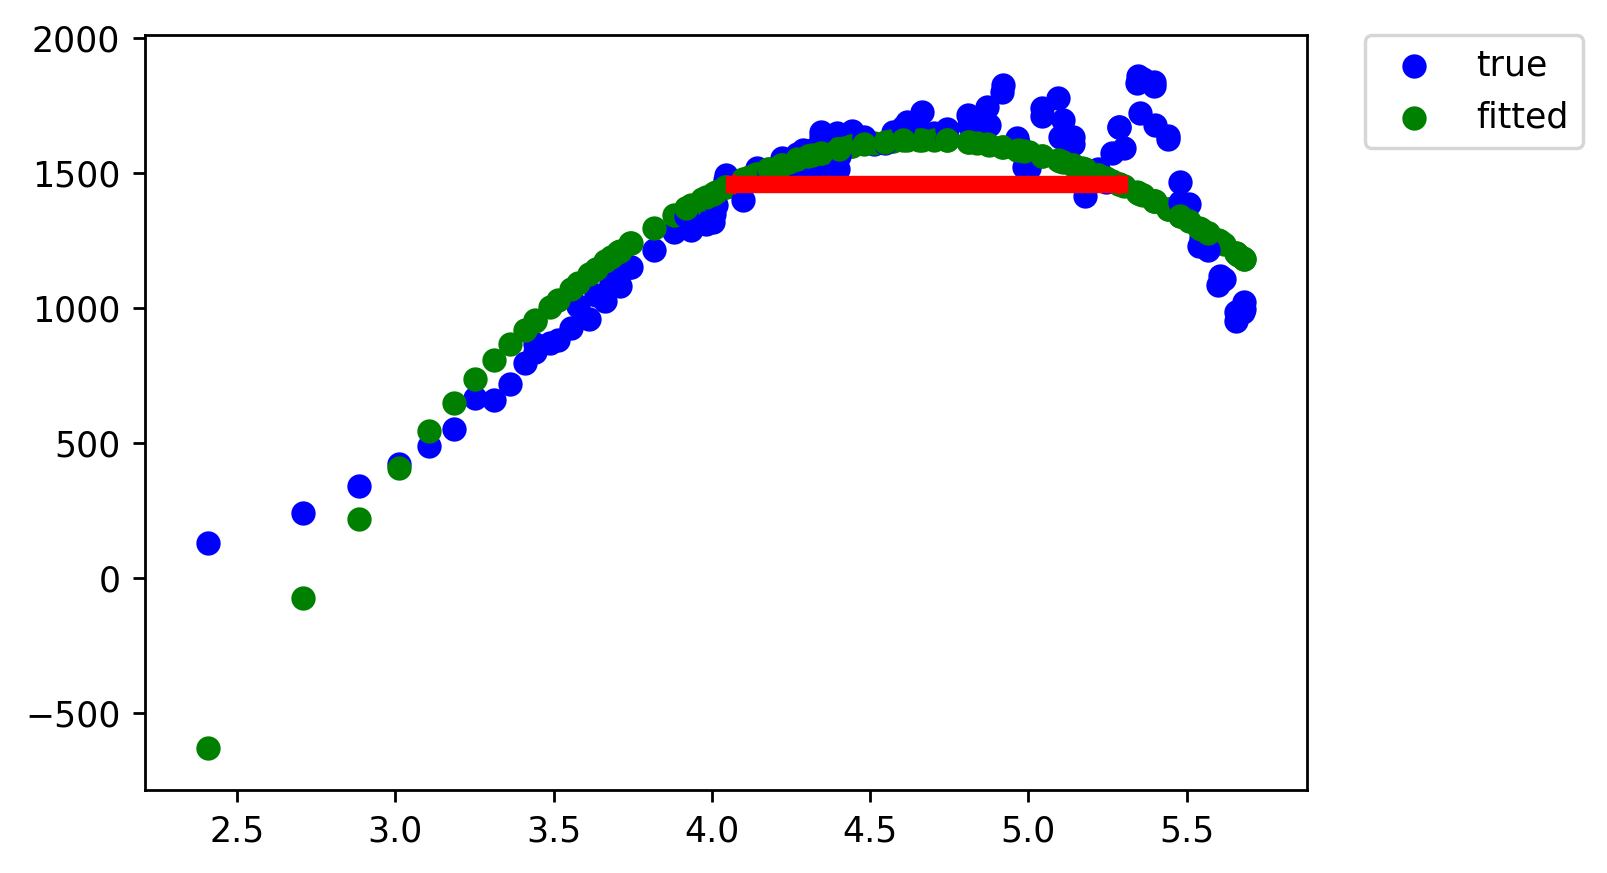
\includegraphics[scale=.3]{images/polyfit/fig_690_total_2_range.png}\label{fig12:a}}
	\subfloat[]{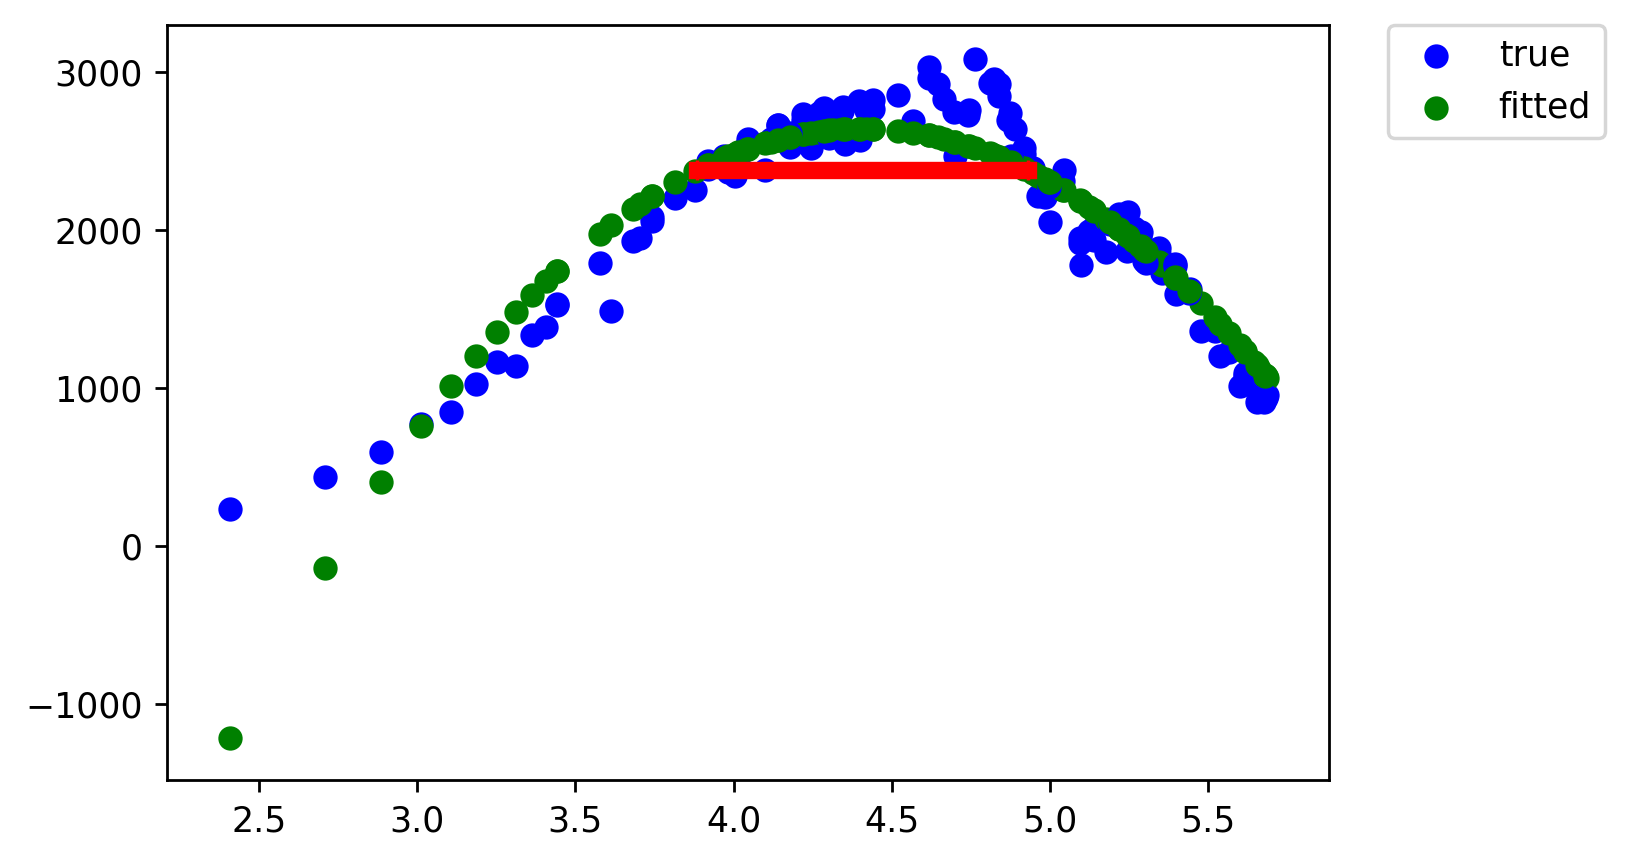
\includegraphics[scale=.3]{images/polyfit/fig_690_total_4_range.png}\label{fig12:b}}
	\subfloat[]{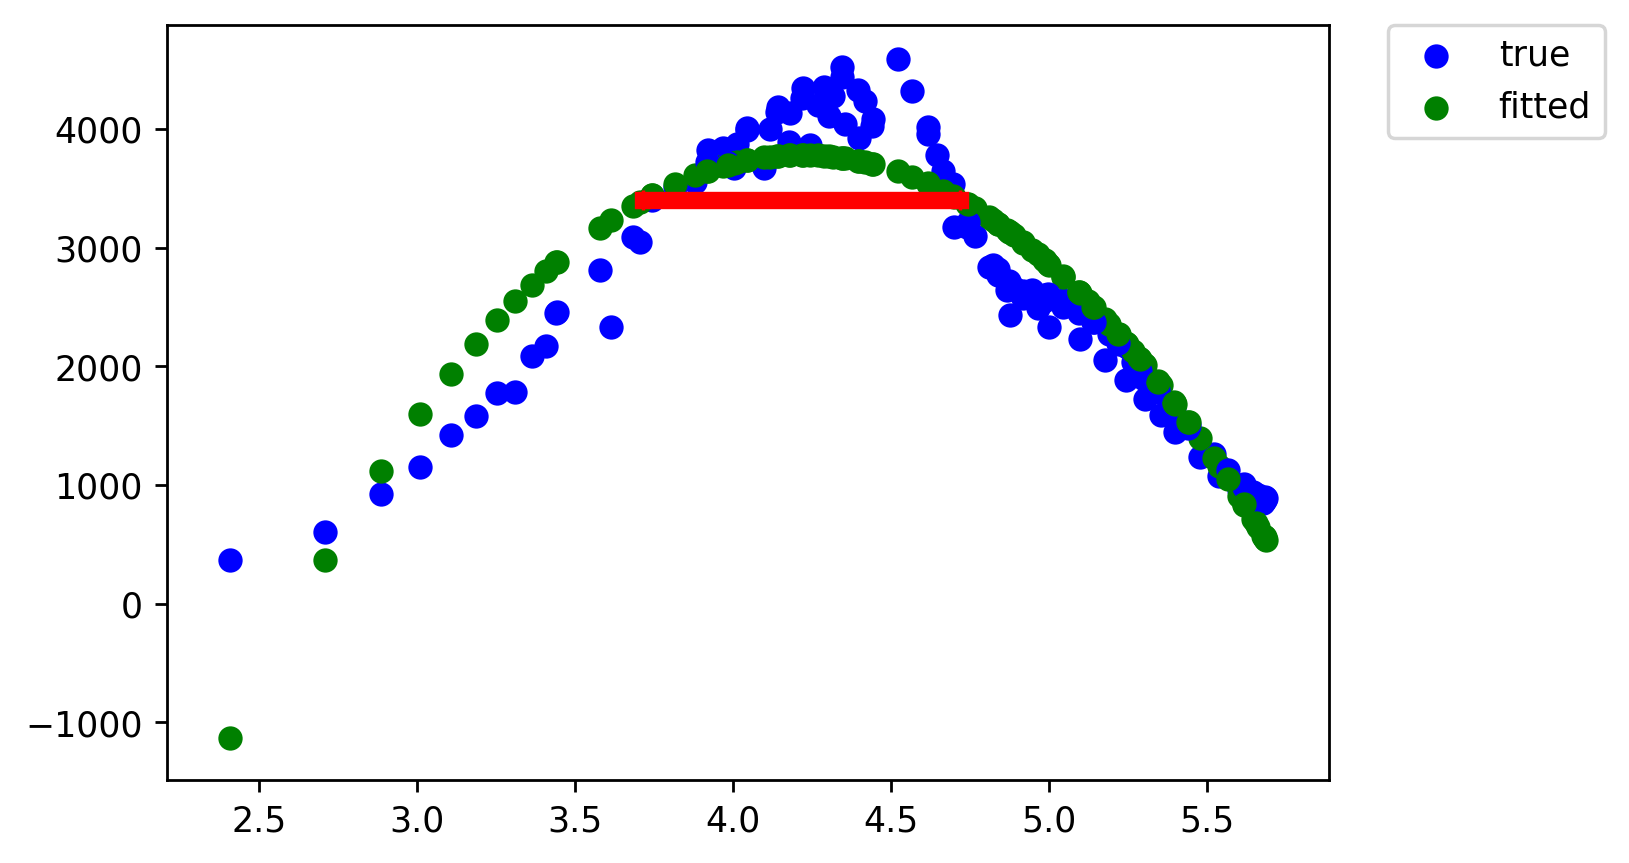
\includegraphics[scale=.3]{images/polyfit/fig_690_total_8_range.png}\label{fig12:c}}
	\caption{The range of grain size (shown as the red line) that leads to a performance within $10\%$ of the maximum performance for (a) 2 cores, (b) 4 cores and (b) 8 cores.}	
	\label{fig12}
\end{figure}


\begin{figure}[H]
	\centering
	\subfloat[]{\hfill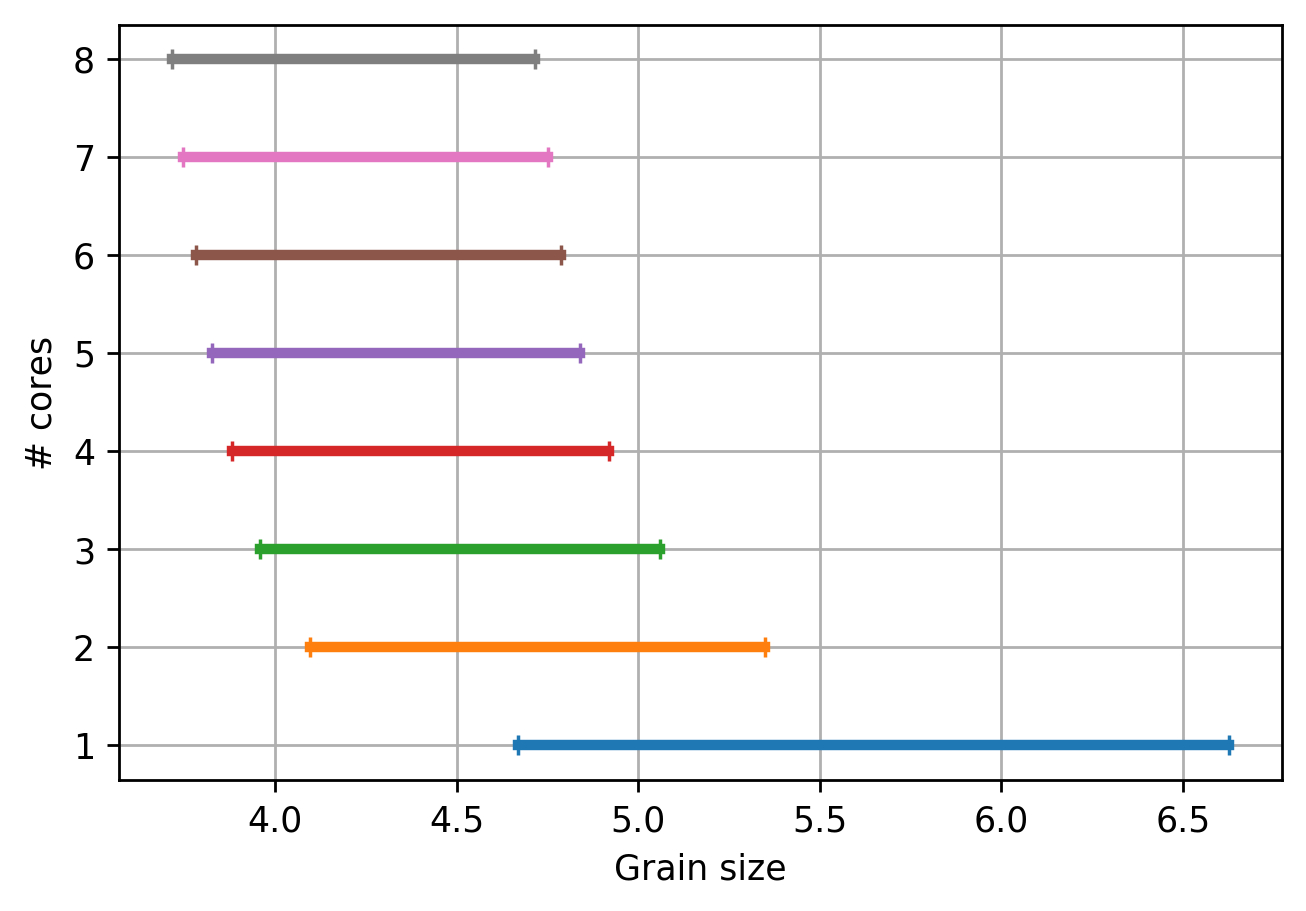
\includegraphics[scale=.5]{images/polyfit/fig_690_peak_range_all.png}\label{fig13:a}}
	\subfloat[]{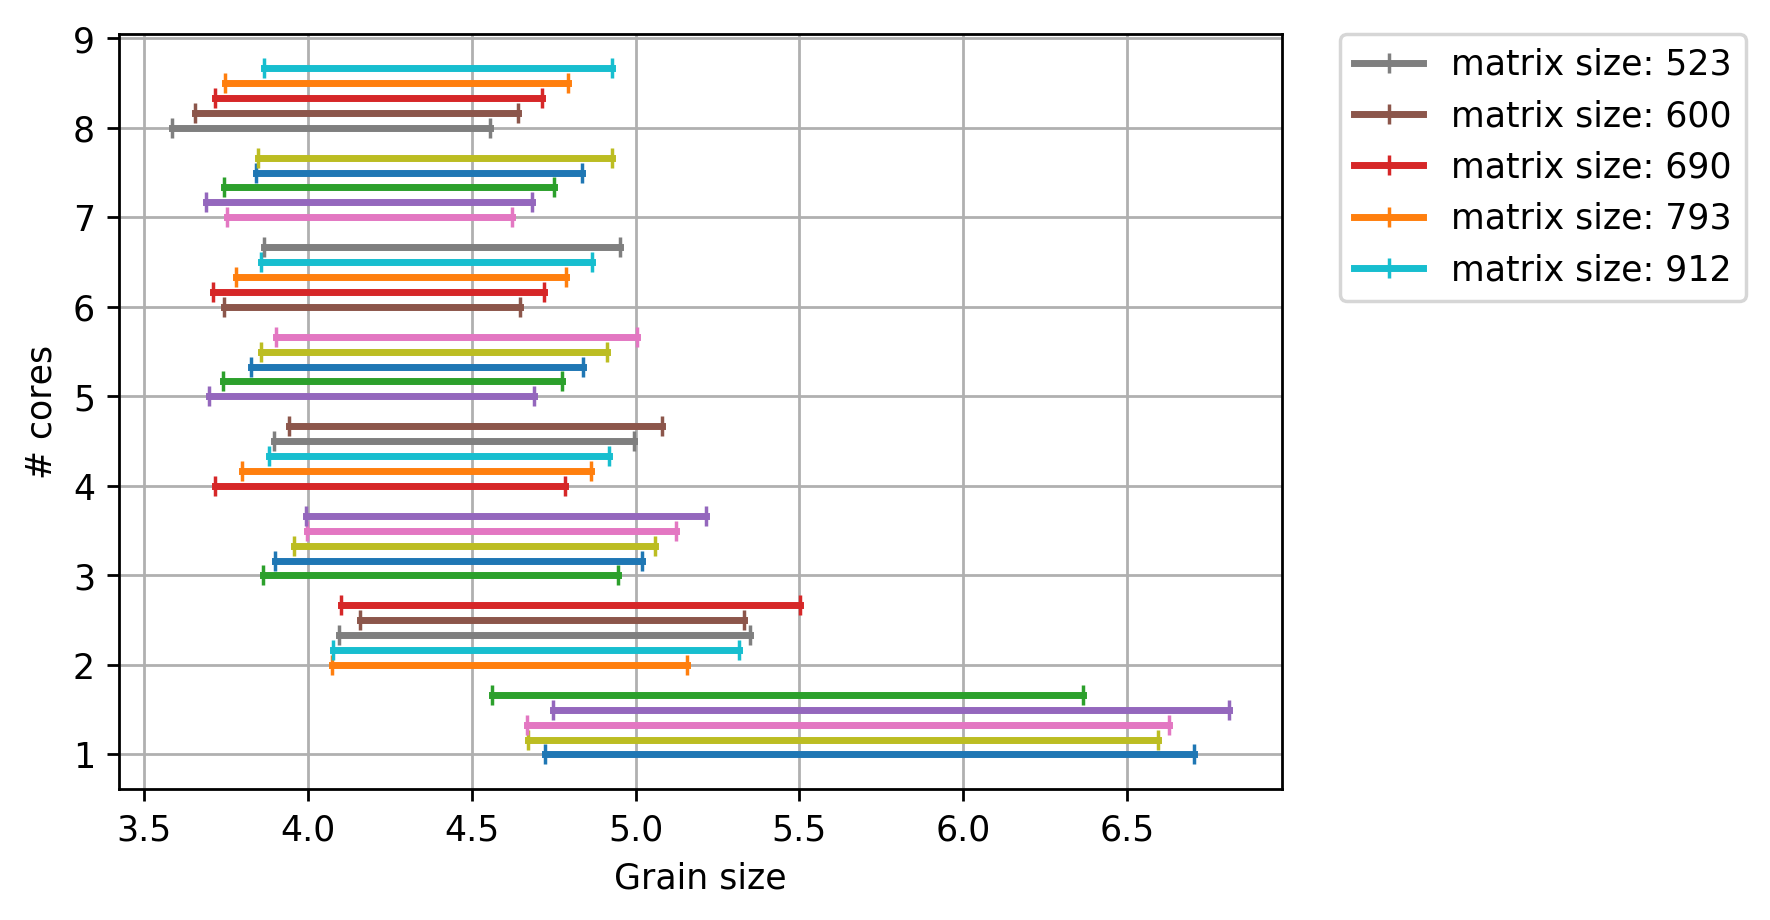
\includegraphics[scale=.5]{images/polyfit/fig_523-912_peak_range_all.png}\label{fig13:b}}
	\caption{The range of grain size within $10\%$ of the maximum performance of the fitted polynomial function for $DMATDMATADD$ benchmark for different number of cores for (a) matrix size $690\times690$ (b)matrix size $523\times523$ to $912\times912$.}	
	\label{fig13}
\end{figure}



Figure~\ref{fig13:a} shows the calculated range for matrix size $690\times690$ for each specific number of threads, while Figure~\ref{fig13:b} compares the range for different matrix sizes. 
\vspace{\baselineskip}	

\subsubsection{Estimating the chunk size}
Once we identified a range of grain sizes that is expected to leads us to highest achievable performances for a specific matrix size and a specific number of cores, the next step is finding the possible combinations of block size and chunk size to achieve that range of grain sizes.  
As stated earlier in this chapter, results obtained from Figure~\ref{fig6} suggests that with a fixed grain size, our choice of block size does not affect the performance directly, as long as there exist a chunk size that when combined by the block size could result in the specified grain size. 

In our experiment, we selected our block size to be $4\times256$. With this assumption, in order for the grain size to be within the specified range for each matrix size, chunk size has to be within a specific range size too.

For example, for a $690\times690$ matrix we calculated the range of maximum performance for $4$ cores to be $[3.88, 4.92]$ in logarithmic scale which is equivalent to $[7586, 83176]$. Setting the block size to $4\times256$, this range forces the chunk size to be within the range $[9,90]$. The range of chunk sizes to match the range of grain sizes identified, and their corresponding throughput is shown in Figure~\ref{fig14}, for matrix size $690\times690$ and block size $4\times256$. The green line is the throughput achieved by the current implementation of HPX backend. Since the graph from the original data is skewed to right, we selected the point after the median of all the chunk sizes in the range, as our candidate chunk size for this specific configuration.


  
\vspace{\baselineskip}	
\begin{figure}[H]
	\centering
	\subfloat[]{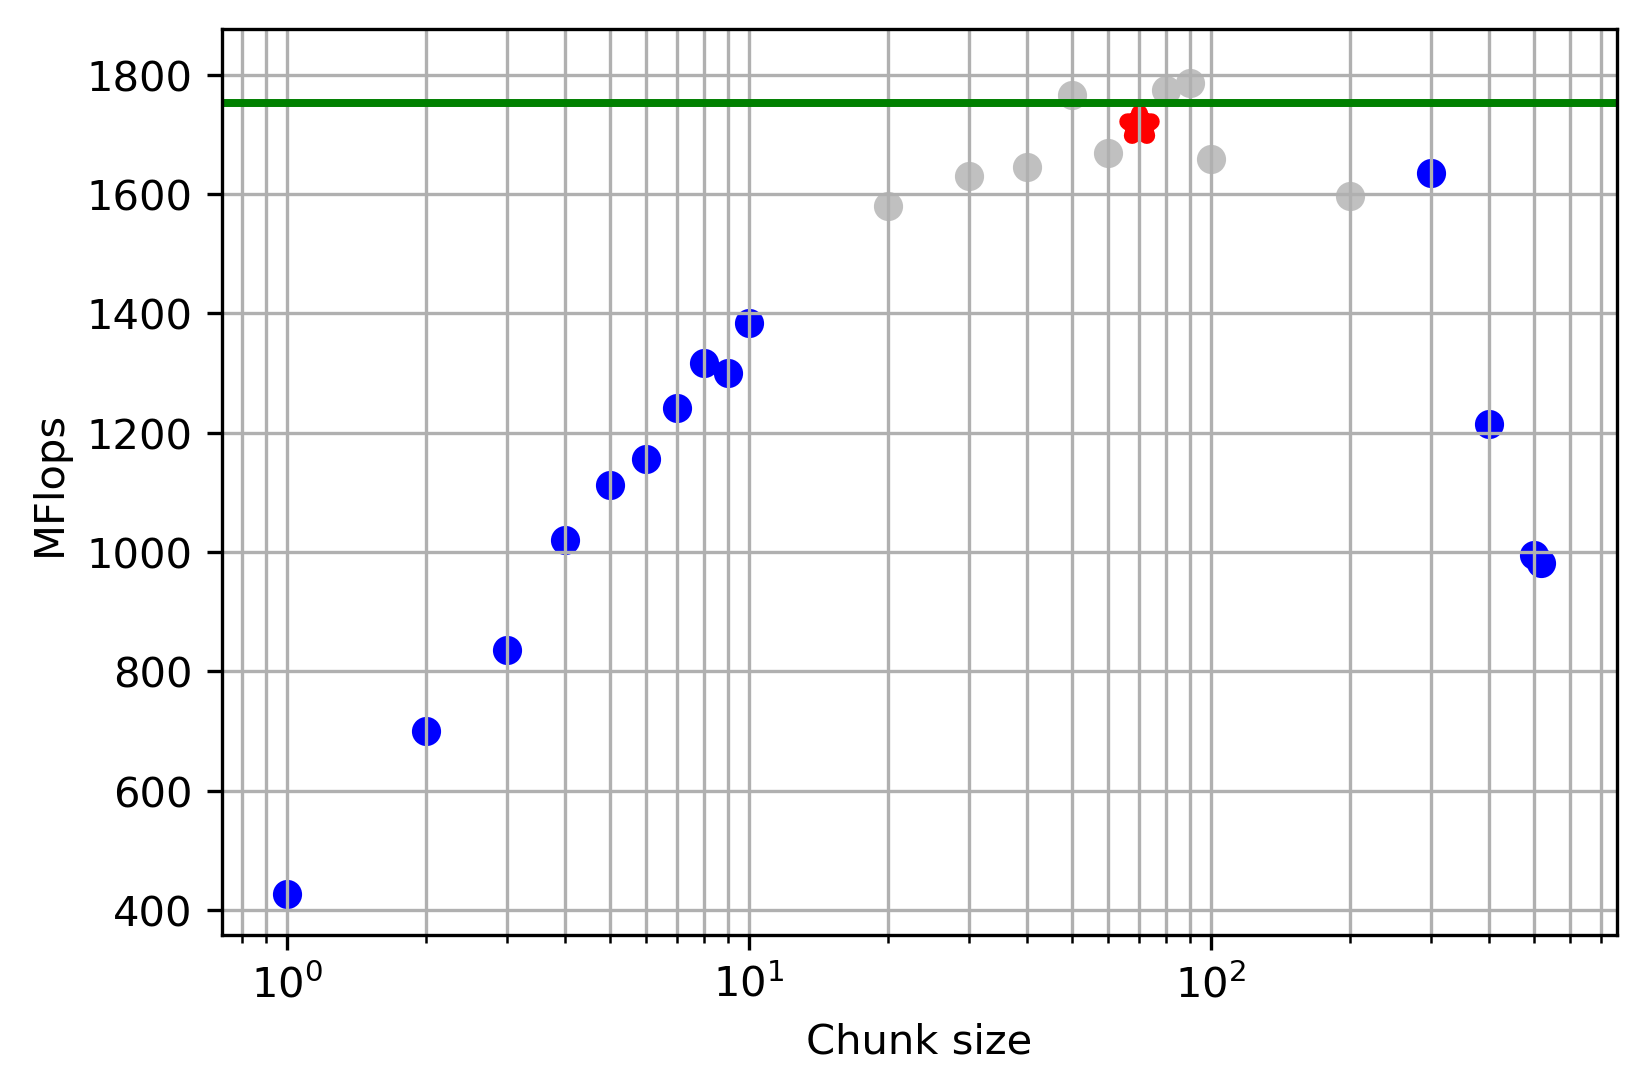
\includegraphics[scale=.35]{images/polyfit/fig_690_chunks_2_4-256.png}\label{fig14:a}}
	\subfloat[]{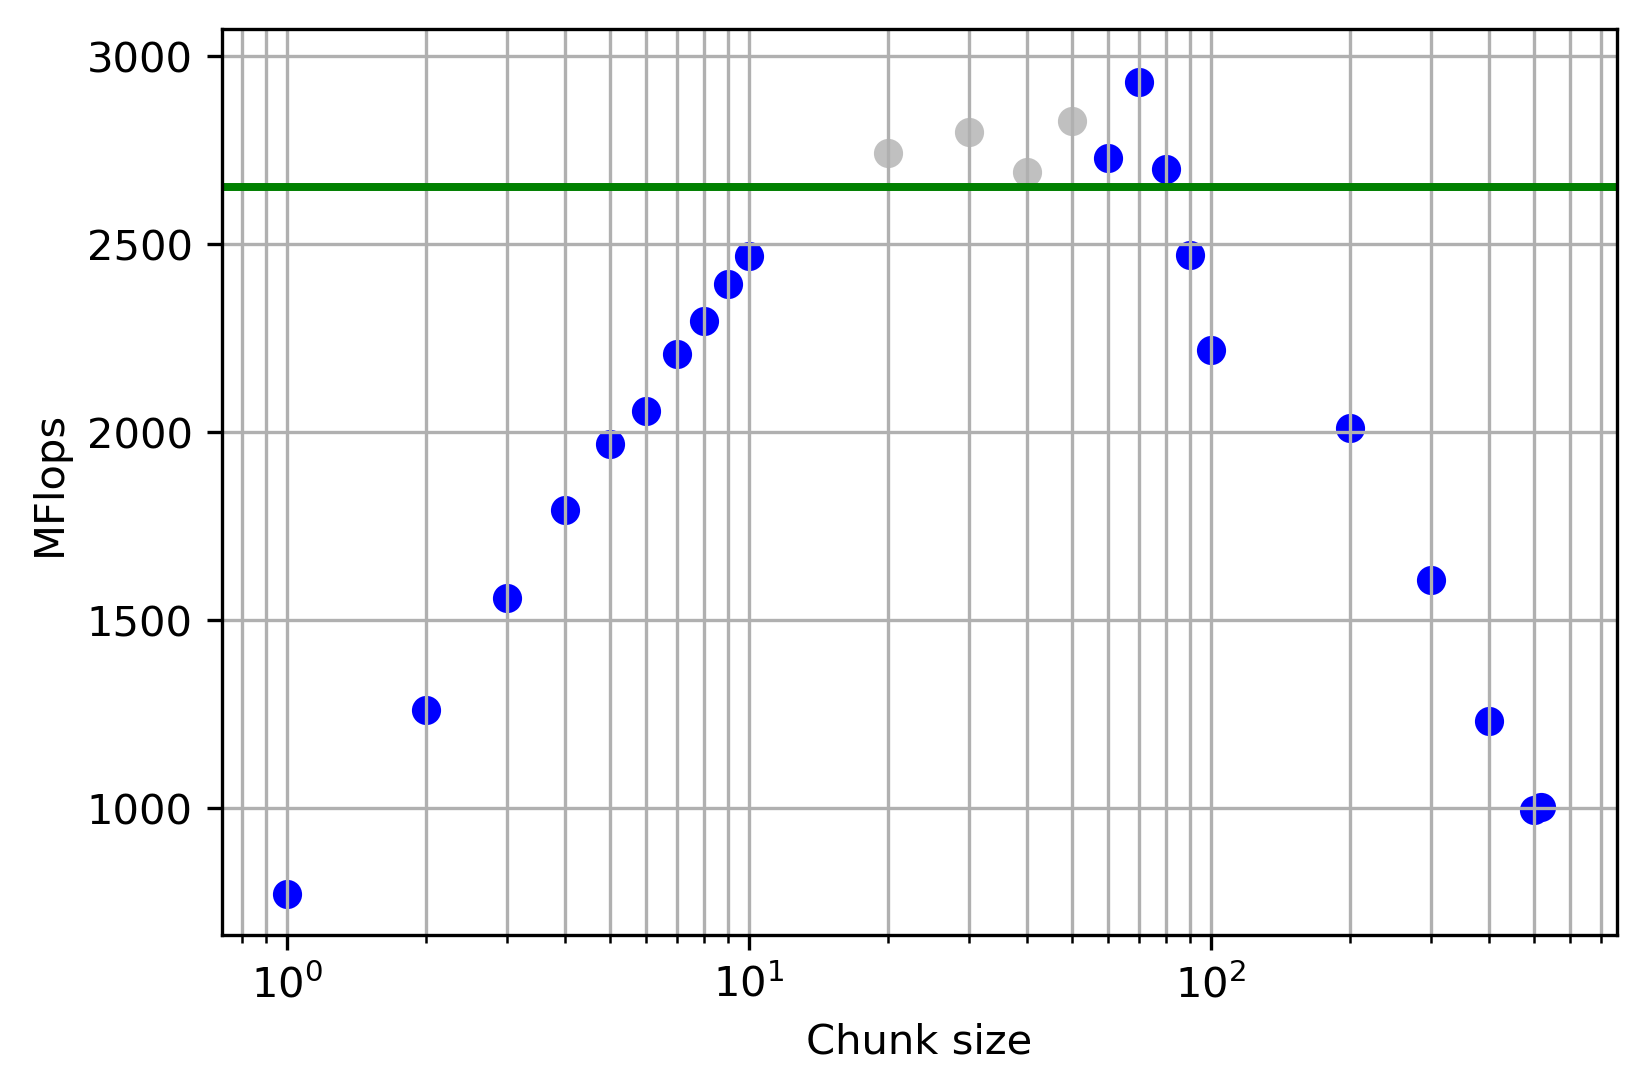
\includegraphics[scale=.35]{images/polyfit/fig_690_chunks_4_4-256.png}\label{fig14:b}}
	\subfloat[]{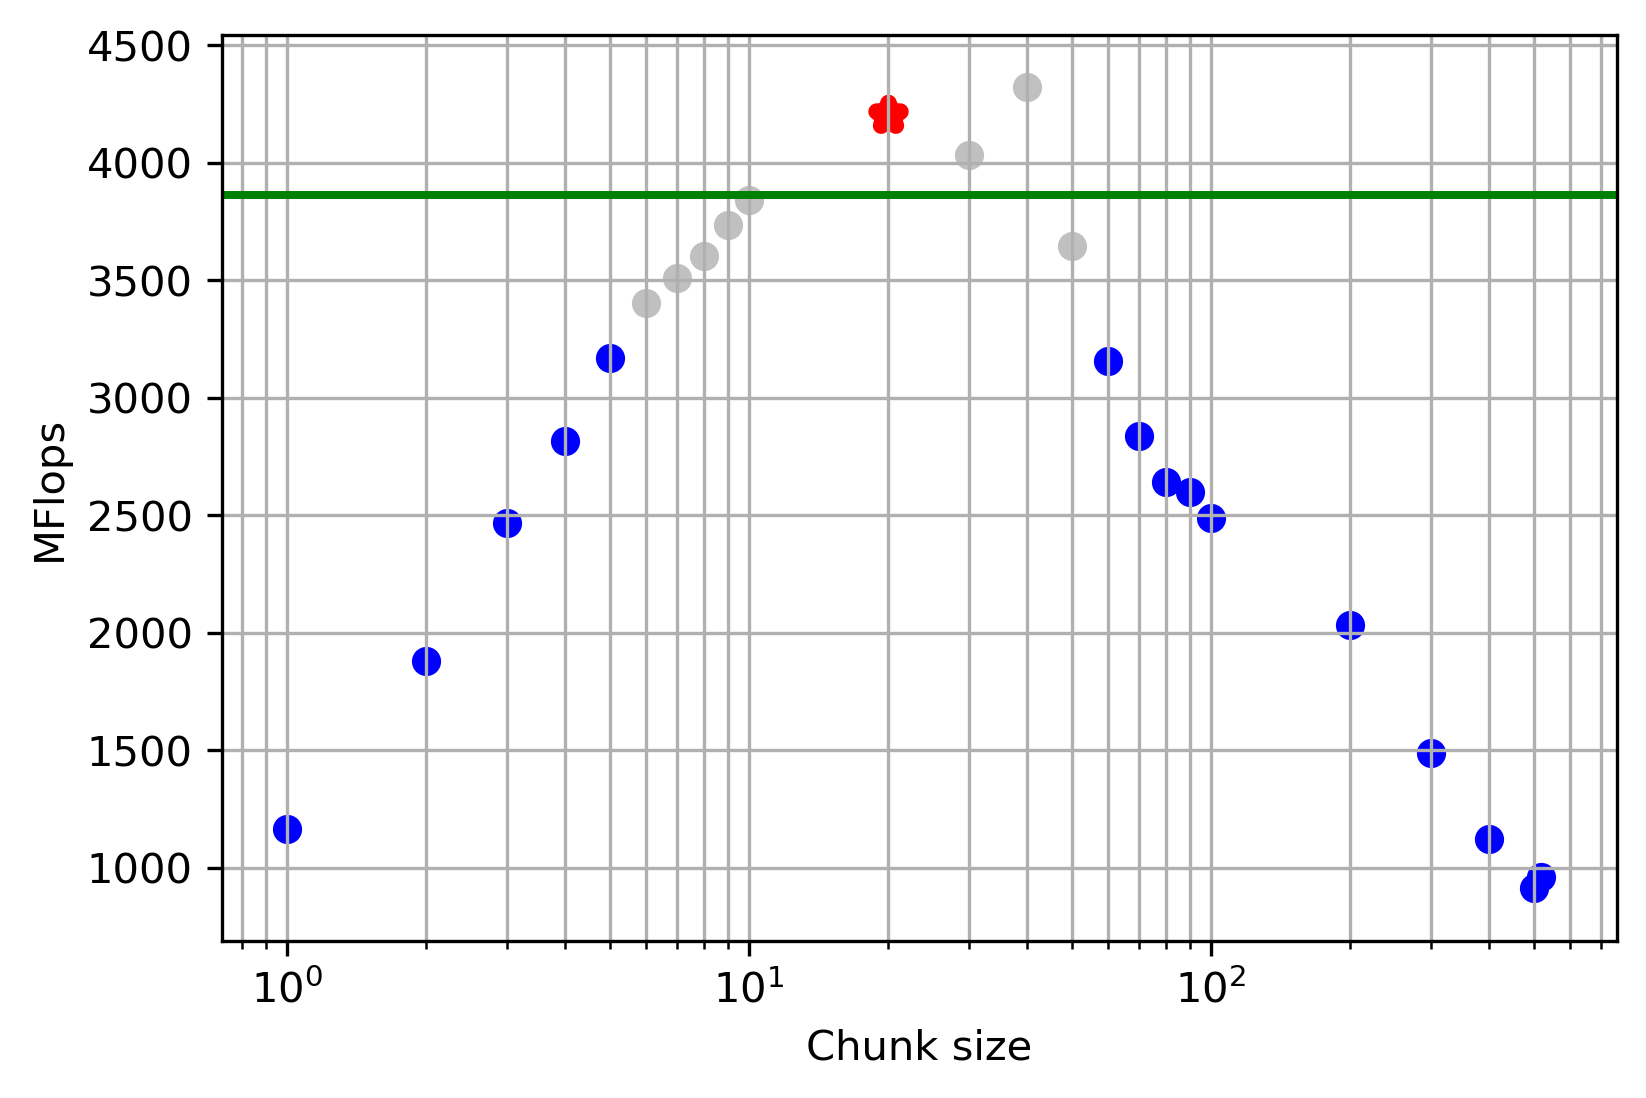
\includegraphics[scale=.35]{images/polyfit/fig_690_chunks_8_4-256.png}\label{fig14:c}}
	\hfill
	\subfloat[]{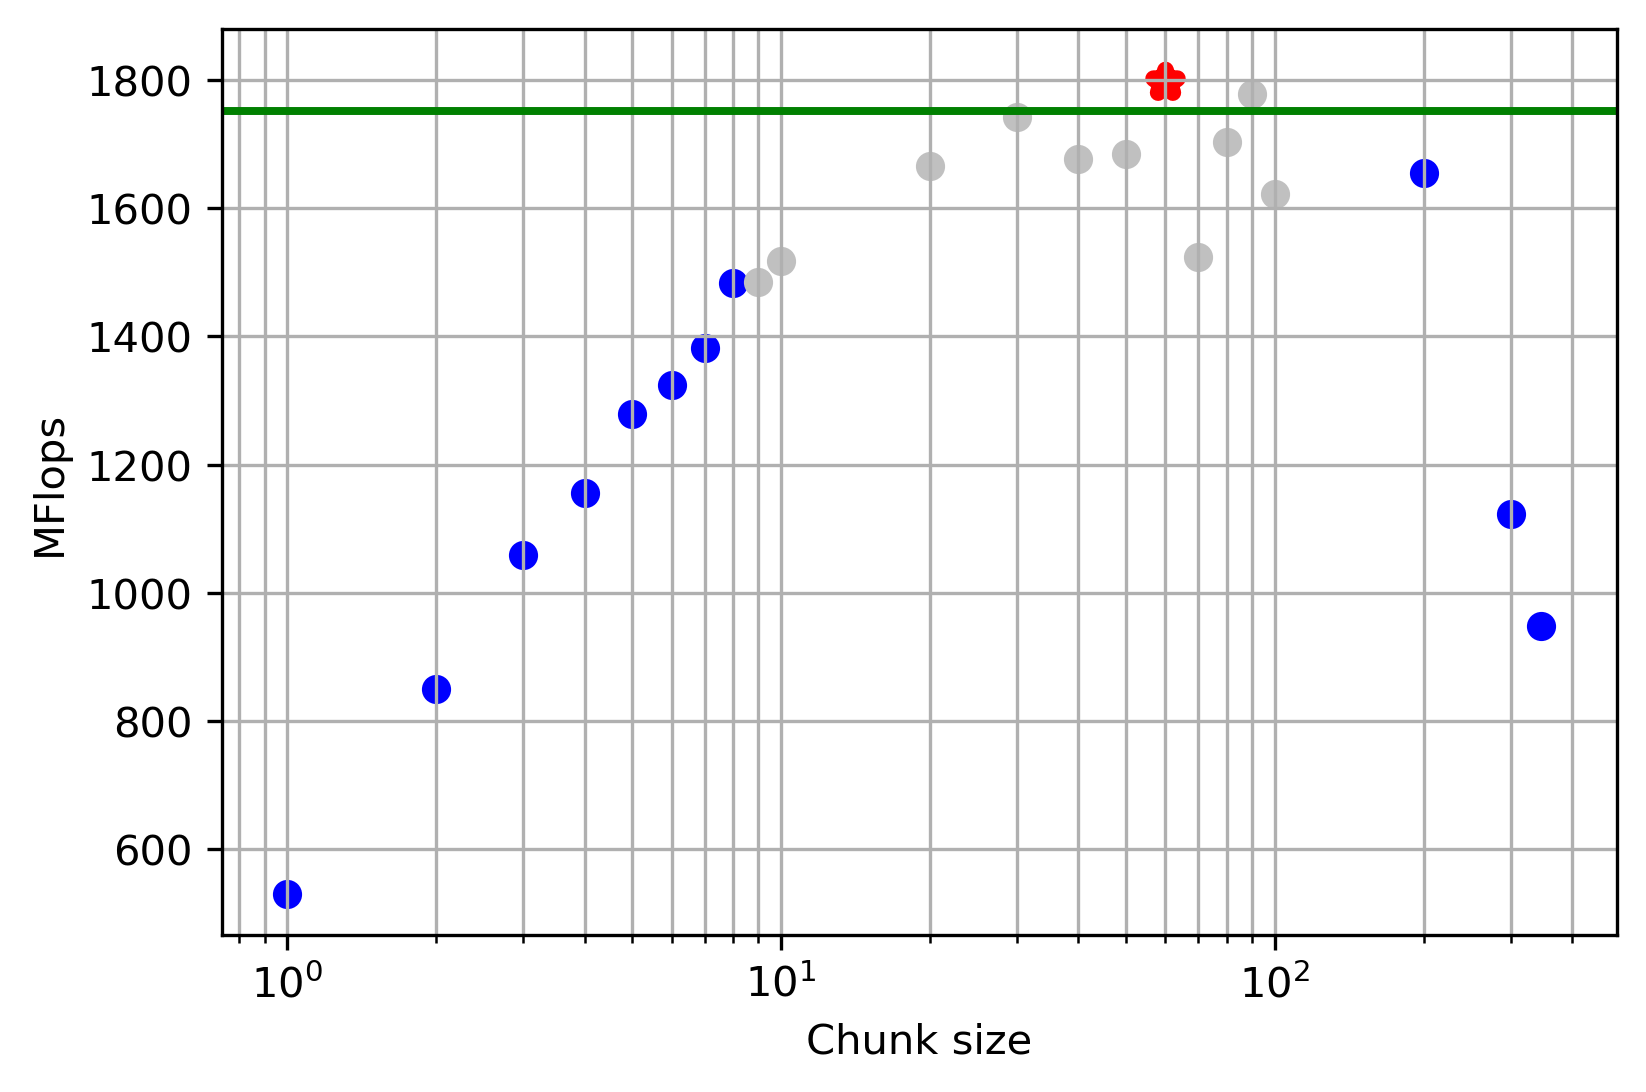
\includegraphics[scale=.35]{images/polyfit/fig_690_chunks_2_4-512.png}\label{fig14:d}}
	\subfloat[]{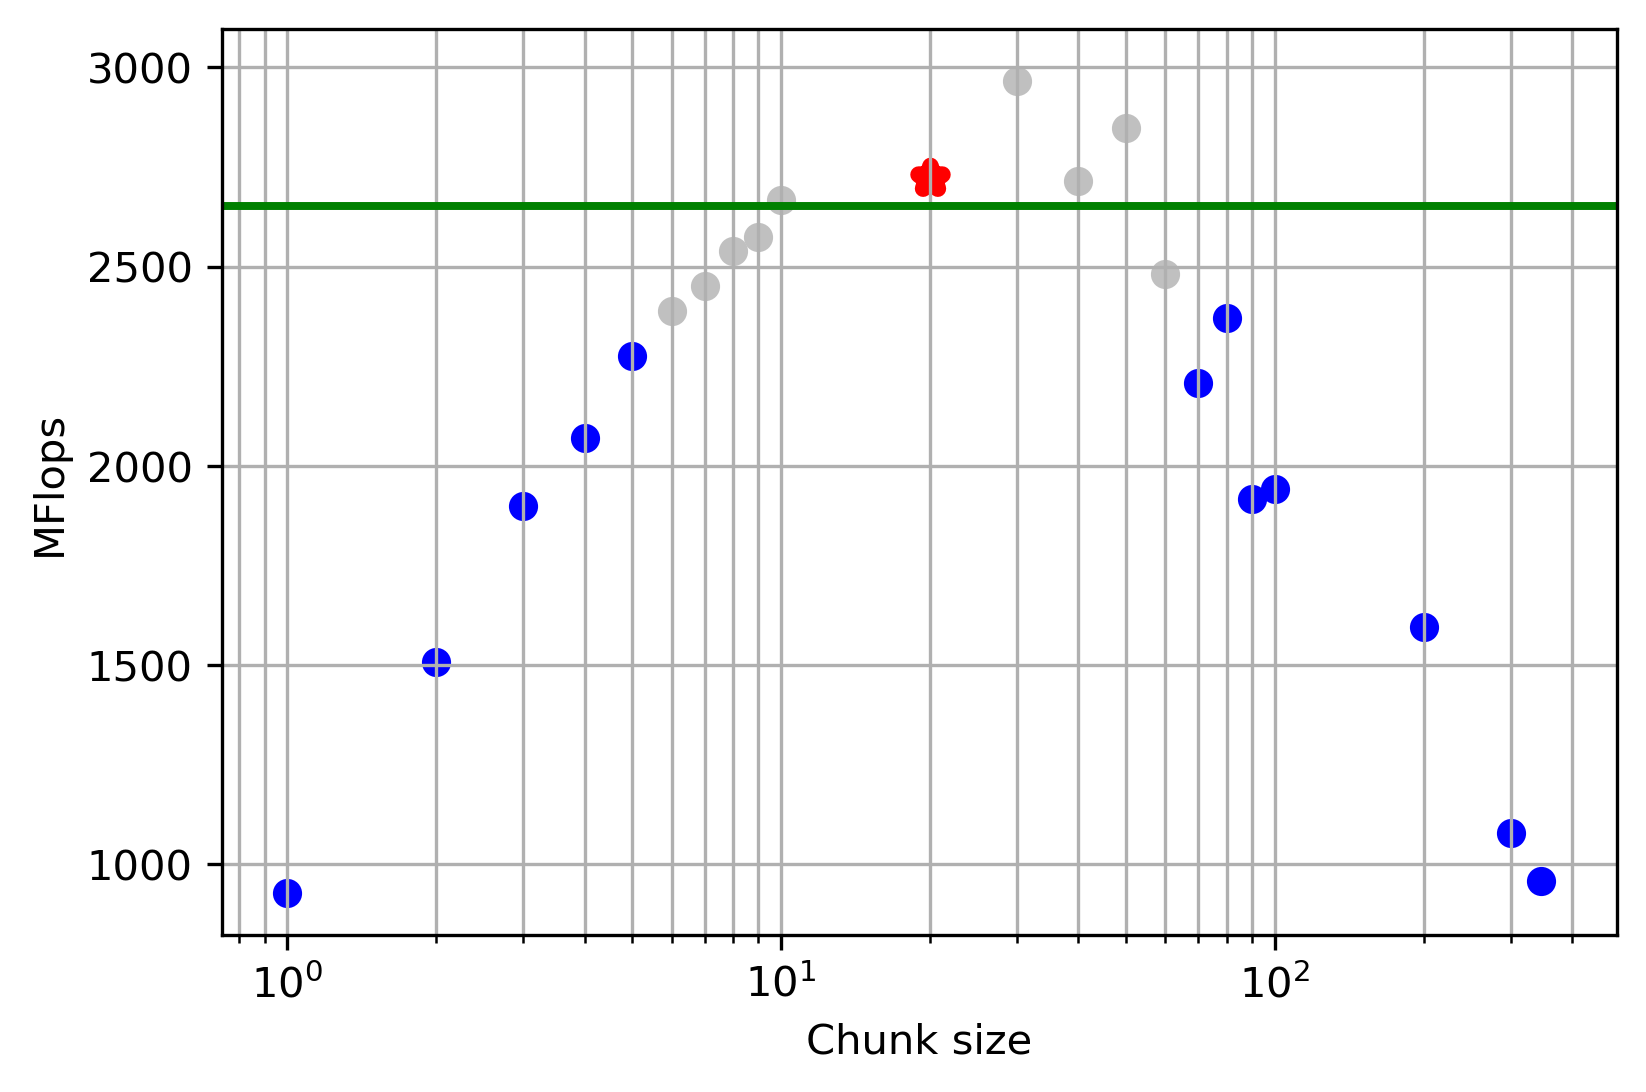
\includegraphics[scale=.35]{images/polyfit/fig_690_chunks_4_4-512.png}\label{fig14:e}}
	\subfloat[]{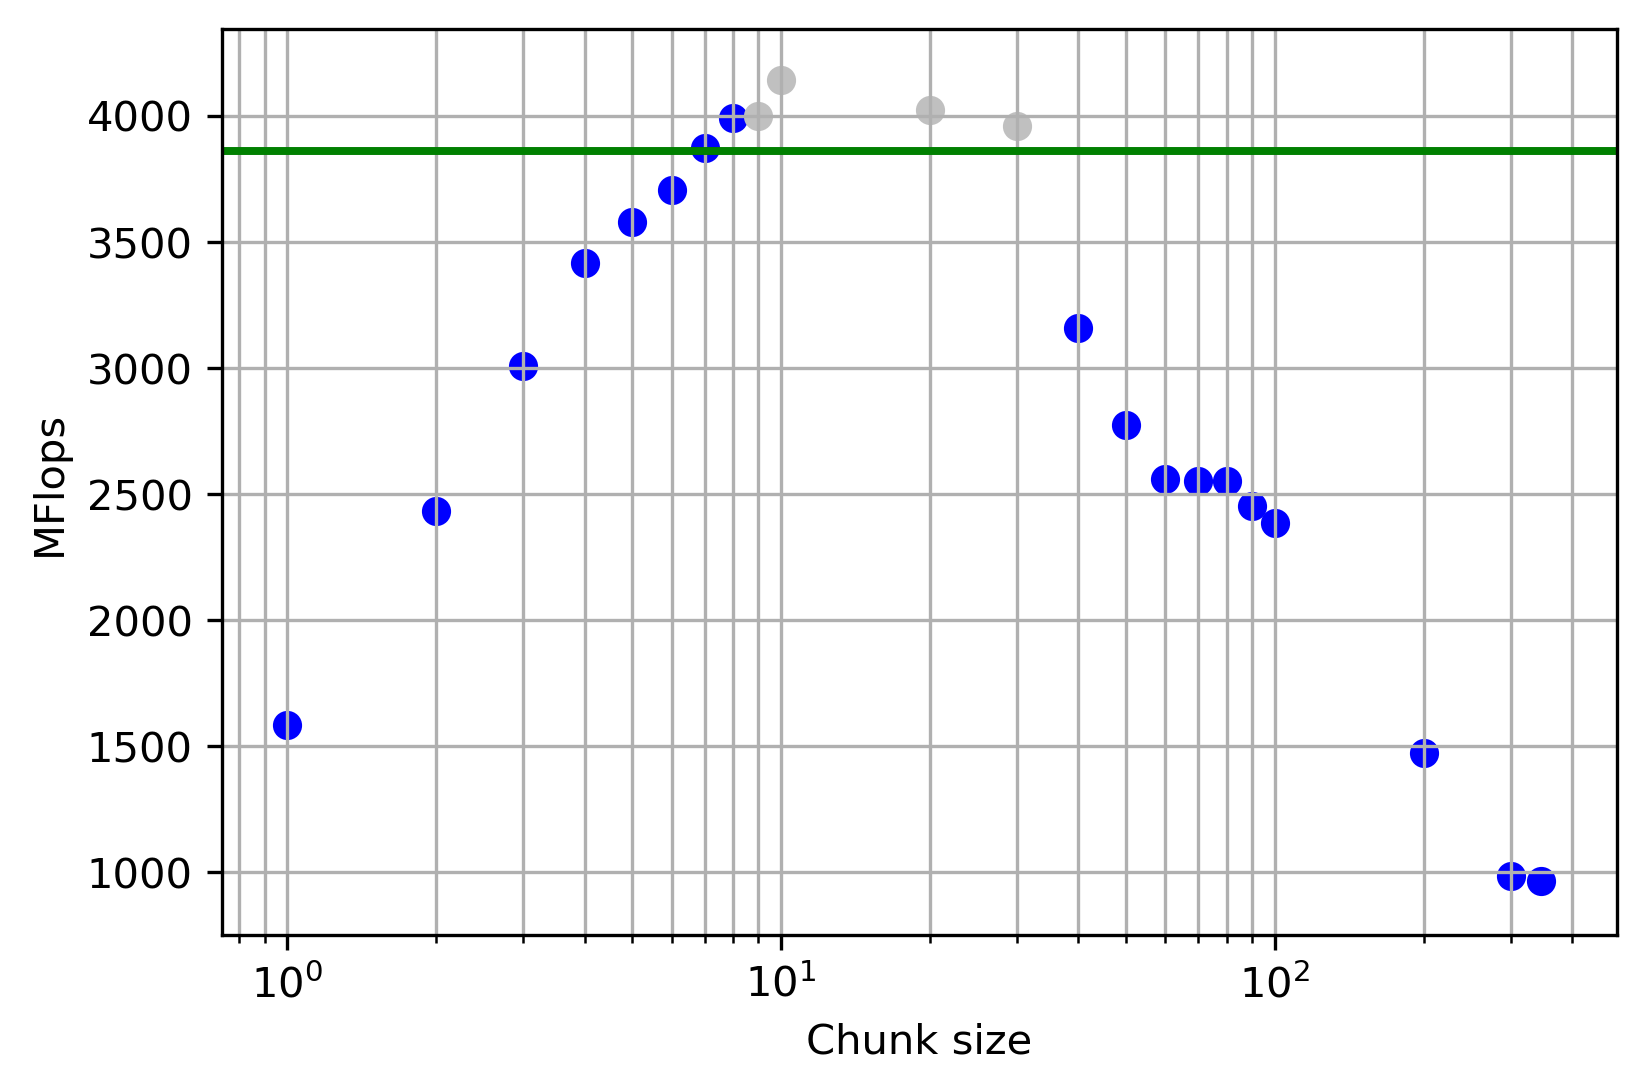
\includegraphics[scale=.35]{images/polyfit/fig_690_chunks_8_4-512.png}\label{fig14:f}}
	\caption{The range of chunk sizes to produce a grain size within $10\%$ of the maximum performance of the fitted quadratic function for $DMATDMATADD$ benchmark for matrix size $690\times690$ with block size of $4\times256$ on (a) $2$ cores, (b) $4$ cores, and (c) $8$ cores, and block size of $4\times512$ on (d) $2$ cores, (e) $4$ cores, and (f) $8$ cores. Silver points denotes the detected range of chunk size, and the red star shows the median point.}	
	\label{fig14}
\end{figure}


\subsection{Bathtub fit}
In the previous section we studied the possibility of using a polynomial to capture the relationship between grain size, number of cores, and throughput for a fixed matrix size, with the purpose of finding a range of grain size that leads us to maximum performance. 
Although the polynomial function was helpful in directing us toward our objective, it does not have a physical implication. 

This motivated us to change our view, and instead of looking just at the data and trying to find a function to fit the data, study the behavior of the data, and then find a function that would be likely to fit the data. That function would be a good fit mostly because that's how we expect the throughput to change with grain size, and not just how the data looks like.   



\pagebreak
\singlespacing

\chapter{Understanding the effect of grain size on concurrency in an asynchronous many-task runtime system}\label{Bathtub}
\doublespacing
\section{Analytical Modeling}
In the previous section we studied the possibility of using a polynomial to capture the relationship between grain size, number of cores, and throughput for a fixed matrix size, with the purpose of finding a range of grain size that leads us to maximum performance. 
Although the polynomial function was helpful in directing us toward our objective of finding the region with maximum performance, it lacked a physical implication, and was not quite able to capture the overall behavior of the system. 

This motivated us to change our view, and instead of looking just at the data and trying to find a function to fit the data, study the behavior of the data, and then find a function that would be likely to fit and explain the data. That function would be a good fit mostly because that's how we expect the throughput to change with grain size, and not solely how the data behaves.   

In this chapter we attempt to understand the effect of grain size on the achievable speedup in an asynchronous many-task runtime system, in order to develop an analytical model for predicting the execution time in an asynchronous many task runtime system. 

We have to note here that even if we were able to identify all the factors affecting the execution time, it is still very hard to find an analytical model describing the relationship between these factors and the execution time. In this chapter we explain our effort in this direction by starting from a simple benchmark. We suggest a formula based on our knowledge of the behavior of the system, and the collected data. Then we will try to generalize the proposed formula to arbitrary for loops with balanced work-load for each iteration. 


Throughout this chapter we will be using the following terms and definitions to simplify our work. We represent the number of cores available with $N$, the number of tasks created as $num\_{tasks}$, the maximum amount of work assigned to one core as $w\_c$, the number of cores that are actually doing the work as $M$ ($M\leq{N}$), the total amount of work available as $problem\_{size}$, and the sequential execution time as $t_{seq}$.

In an attempt to find this analytical model, we started with looking into two major factors, the overhead of creating tasks, and the maximum amount of work assigned to one core. 
In order to understand how these factors contribute to the execution time, we created a benchmark based on a simple \textit{for\textunderscore{loop}} with different number of iterations, iteration lengths, and chunk sizes, as shown in Listing~\ref{hpx_for_loop}. 
Each iteration consists of a while loop that makes sure the iteration lasts a certain amount ot time. This way, knowing how long it would take to execute one iteration(denoted as \textit{iter\textunderscore{length}}), how many of iterations are executed by one HPX thread(denoted as \textit{chunk\textunderscore{size}}), and finally how many iterations there are(denoted as \textit{num\textunderscore{iterations}})), we can see how the execution time changes when the problem is executed on different number of cores. Here, we define \textit{problem\textunderscore{size}} as the time it takes to execute all the iterations, which is:

\begin{equation}\label{problem_size}
problem\_size = iter\_length\times{num\_iterations}
\end{equation}

The total execution time could be assumed to be roughly the amount of time it takes for the core with the maximum amount of work to finish it's job. Here we call the core with maximum expected amount of work as $core_0$, and the associated amount of work as $w\_c$. 
With this assumption, the main factors contributing to the execution time for this simple problem are the overhead of creating tasks on $core_0$, the time it takes to run $w\_c$ amount of work on $core_0$, and the number of cores that will be executing the work($M$). 


Formula~\ref{formula31} shows the expected formula in it's simplest form, with $q$ as a constant factor to account for unknown factors.  

\begin{equation}\label{formula31}
\begin{aligned}
&execution\_time = 
t\_{overhead}\:\:+\:\:w\_c\:\:+\:\:q
\end{aligned}
\end{equation}

Where, 
\begin{equation}\label{formula2}
w\_c =\left\{
\begin{aligned}
&problem\_{size} \:\:\:\:\:\:\:\:\:\:\:\:\text{ if } N=1\\
&problem\_{size}-g\times{(N-1)}\times(\left \lceil{\frac{num\_{tasks}}{N}}\right \rceil-1) \\
&\:\:\:\:\:\:\:\:\:\:\:\:\:\:\:\:\text{if }num\_{tasks}\%N=1\text{\:\:\&\:\: }num\_{iterations}\%chunk\_{size}\neq0\\ 
%\text{\:\:or} \\ g\times(\left \lceil{\frac{num\_{tasks}}{M}}\right \rceil-1)+(num\_{iterations}\%chunk\_{size})\times(iter\_{length}) \\ \:\:\:\:\:\:\:\:       
&g\times\left \lceil{\frac{num\_{tasks}}{N}}\right \rceil  \:\:\:\:\:\:\:\:\:\:    \text{otherwise}
\end{aligned}
\right.
\end{equation}

In this formula $t\_{overhead}$ represents the penalty that we have to pay for running the program in parallel. We hold three major factors accountable for this overhead. 

The first factor is the overhead of creating the tasks. The overhead of creating one task itself is small, but as the number of created tasks becomes larger, it becomes significant.
When $num\_{tasks}$ tasks are created, $\left\lceil{\frac{num\_{tasks}}{N}}\right \rceil$ tasks would be created on $core\_0$. If we represent the overhead of creating a task on one core with $\alpha$, the portion of $t\_{overhead}$ resulted from creating tasks could be stated as $\alpha\times{\left\lceil{\frac{num\_{tasks}}{N}}\right \rceil}$.

The second factor is the overhead of managing the created tasks. While the overhead of creating a task should be constant on a specific machine architecture, we are suggesting here that the overall overhead of managing $num\_{tasks}$ tasks, is a factor($\delta$) of $N$. This effect is originated from HPX's strategy to avoid allocating new stacks by keeping the previous stack alive until new thread is created, at that point the stack is assigned to the new thread. 
The overhead of managing a task on a machine is shown with $\delta\times{num\_{tasks}}$.

The third factor is the overhead caused by work stealing. Although work stealing is a very helpful method to achieve balanced loads, it induces an overhead due to constant efforts of idle cores to steal work from the other cores. Each of these efforts would result in trashing the local cache of the busy cores. This effect helps for load balancing when the number of tasks created is greater than or equal to the number of cores, but as the number of tasks get smaller than the number of cores, the unsuccessful steal efforts become more noticeable.

HPX by default uses the priority local scheduling policy which creates one queue for each OS thread. When there is no more work left in on core's queue, it will attempt to steal work from other cores starting from it's neighbors. If the attempt is not successful, it will move to the next level neighbors. This continues until the core that initiates the steals(called the thief) is able to find a core with tasks in their queue which can can be stolen(called the victim). 

There is an optional command line option ${--hpx:numa-sensitive}$ to make sure that the thief would try the queues of the cores in the same NUMA domain first. This option is provided based on the fact that it is much faster to access the local memory of a processor than the local memory of another processor.  
%In our example we are only using 8 cores from the same NUMA domain 
  
Based on the mentioned factors, Formula~\ref{formula31} then becomes:

\begin{equation}\label{formula32}
\begin{aligned}
&execution\_time = 
\alpha\times{\left\lceil{\frac{num\_{tasks}}{N}}\right\rceil\:\:+\:\:\delta\times{num\_{tasks}}\:\:+\:\:t\_{overhead\_{ws}}\:\:+\:\:w\_c+\:\:q}
\end{aligned}
\end{equation}



 
%On the other hand, when number of tasks created is smaller than the number of cores, we observe continuous efforts from the idle cores to steal work from cores that are actually doing the work, interrupting the cache coherency constantly. We represent this effect with $\delta\times{(N-M)\times{M}}\times{num\_{tasks}}\times{\frac{1}{M}})$.

  

%\begin{equation}\label{formula1}
%\begin{aligned}
%&execution\_time = \\
%\left\{
%\begin{aligned}
%&
%\alpha\left\lceil{\frac{num\_{tasks}}{M}}\right \rceil +\beta\times{(N-1)}{num\_{tasks}}+{w\_c+\gamma\times{w\_c}\times{(M-1)}} \:\: \text{if\:\:}num\_{tasks}>N\\
%&\alpha\left \lceil{\frac{num\_{tasks}}{M}}\right \rceil +\delta\times\frac{num\_{tasks}-1}{N}+{w\_c+\gamma\times{w\_c}\times{(M-1)}} \:\: \text{otherwise}
%\end{aligned}
%\right.
%\end{aligned}
%\end{equation}
%\vspace{\baselineskip}



As discussed in chapter~\ref{Background}, Amdahl's law and Universal Scalibility Law, suggest that, for a fixed problem size, as we increase the number of cores in a multicore system, we do not observe a linear speedup, which is mainly resulted from latency and coherency.
Universal Scalibilty Law\cite{gunther2007guerrilla} suggests that an overhead associated with the number of cores should be added to the expected execution time. We added a term to Formula~\ref{formula2} to represent this effect. Moreover, we adjusted the formula by changing the total number of cores ($N$) to the number of cores that are actually executing the work ($M$). 
Assuming we are running our application on $N$ cores, with a grain size equal to $g$, $num\_{tasks}$ tasks are being created, and $M$ cores are actually doing the work. If $num\_{tasks}<N$, $M$ would be equal to $num\_{tasks}$, otherwise $M=N$.

\begin{equation}\label{formula19}
M=\left\{
\begin{aligned}
&num\_{tasks} \text{\:\:\:\:if \:} num\_{tasks}<N\\
&N \text{\:\:\:\:otherwise}
\end{aligned}
\right.
\end{equation}


Formula~\ref{formula2} is then changed into:

\begin{equation}\label{formula1}
\begin{aligned}
execution\_time = 
\alpha\times{\left\lceil{\frac{num\_{tasks}}{N}}\right\rceil}\:\:&+\:\:w\_c\:\:+\:\:\gamma\times{w\_c}\times{(M-1)}\:\:\\
&+\:\:\delta\times{num\_{tasks}}\:\:+\:\:t\_{overhead\_{ws}}\:\:+\:\:q
\end{aligned}
\end{equation}

Here $t\_{overhead\_{ws}}$ represents all the overhead created due to work stealing. We did some investigations on where this term is originated from for a more precise modeling, but we were not successful. In order to study this effect, we ran a set of experiments while work stealing was turned of. This is possible through adding the command line option \emph{--hpx:queuing = static-priority}.

Figure~\ref{fig40} highlights the effect of work stealing for $problem\_size=3000$ on 4 and 8 threads. As it can be observed, in the region where the number of tasks created is same as the number of cores, this effect is more significant. Although we are not sure how work stealing is causing this effect, \textcolor{red}{we can use a term with Normal distribution with $\mu=\frac{ps}{N}$. We believe this term is originated from HPX's implementation of work stealing, and although it affects the execution time at certain points, since it only adds to the execution time at those points, and our interest is finding the flat region of the graph with the minimum execution time, at this point and for this purpose we could ignore this term in our upcoming calculations.}  


\vspace{\baselineskip}	
\begin{figure}[H]
	\centering
	\subfloat[]{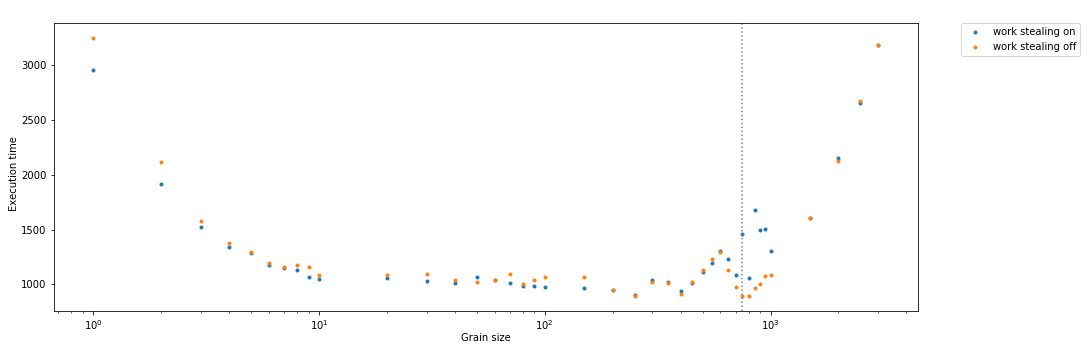
\includegraphics[scale=.4]{images/hpx_for_loop/3000_4_1_all.png}\label{fig40:a}}{\hfill}
	\subfloat[]{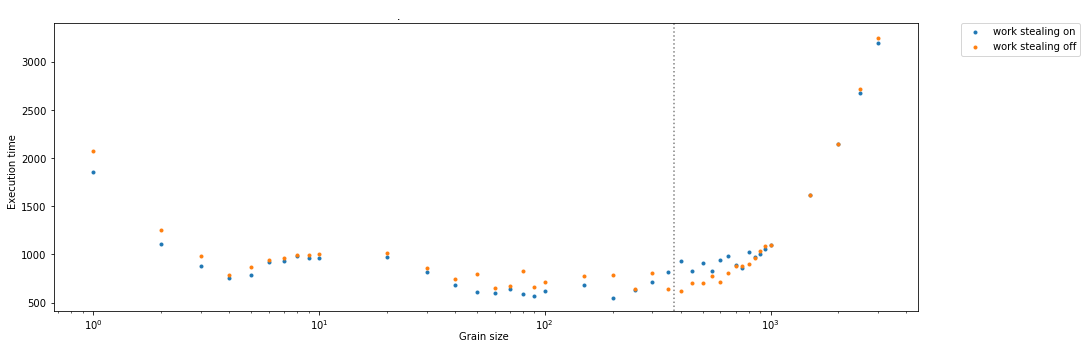
\includegraphics[scale=.4]{images/hpx_for_loop/3000_8_1_all.png}\label{fig40:b}}
	\caption{The results of running the benchmark in Listing with $problem\_size=3000$, on different (a)4 cores, and (b) 8 cores. The vertical dotted line shows the grain size that would generate same number of tasks as the number of cores, with the same amount of work for all the cores.}\label{fig40}		
\end{figure}
 
 
 
Figure~\ref{fig39} shows an example of the results obtained from running the benchmark, for $problem\_size=10000$, on different number of cores.

\vspace{\baselineskip}	
\begin{figure}[H]
	\centering
	{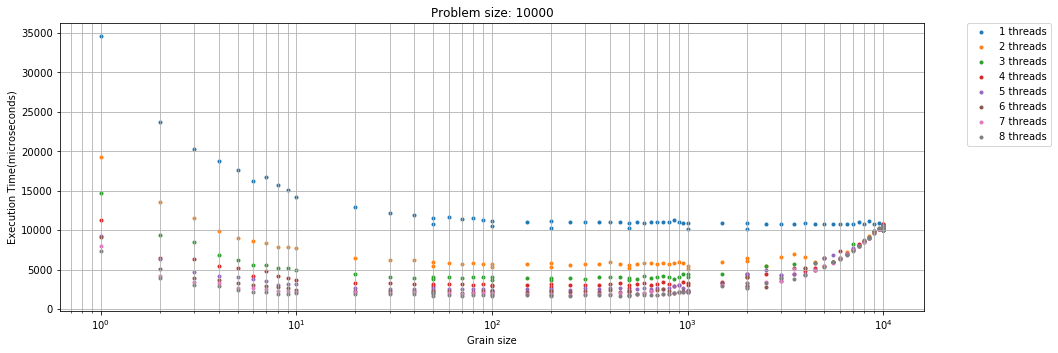
\includegraphics[scale=.45]{images/hpx_for_loop/10000_8_all.png}}
	\caption{The results of running the benchmark in Listing with $problem\_size=10000$, on different number of cores.}\label{fig39}		
\end{figure}

As stated in Chapter~\ref{Background}, at the right hand side of the graph in Figure~\ref{fig39}, the number of tasks created is smaller than the number of cores which results in making at least one of the cores idle, while the other cores are assigned a rather big chunk of work. The performance degradation we observe in that points is associated with starvation, meaning that we are not utilizing our computation resources to the full extent. In these points, the number of cores actually doing the work is equal to the number of the tasks, since each core gets to execute at most one task. At this region of the graph, the maximum assigned work to a core ($w\_c$) is the dominant factor.   

On the other hand, on the left hand side of the graph, since the grain size is very small we end up with creating a large number of tasks. Since there is an overhead associated with each created task, we observe a performance degradation in that region. As the grain size increases, the number of created tasks, and the overhead associated to that decreases consequently. At this region of the graph, the overhead of creating and managing the tasks is the dominant factor.   

To summarize, for this simple experiment, where we do not have to deal with the cash effects, we believe the important factors are: number of HPX threads being created, number of cores the program is ran on, the maximum amount of work one core has to perform. 

The maximum number of tasks assigned to one core, and the number of cores that are actually performing the work, are two other important factors that can be deducted from the aforementioned factors. 


\vspace{\baselineskip}
\subsection{Validating the Proposed Model}
In order to test how the well the suggested model could fit the data, we collected a considerable amount of data with different configurations of number of cores($N$), number of iterations(\emph{num\_{iterations}}), and chunk size($chunk\_{size}$). We set $iter\_{length}$ to $1\mu\text{sec}$ for simplification. For each $num\_{iterations}$, we change the $chunk\_{size}$ from 1 to $num\_{iterations}$ in logarithmic scale. Each of these runs was executed for $N=1,2,3,...,8$.  

As an example, for $problem\_{size}=100000$, we have collected 64 data points for each $N=1,2,...,8$, resulting in $512$ data points in total. Figure~\ref{fig41} shows the execution time for different grain sizes ranging from 1 to 100000 for $problem\_{size}=100,000$ with $N=8$.



\begin{figure}[H]
	\centering
	{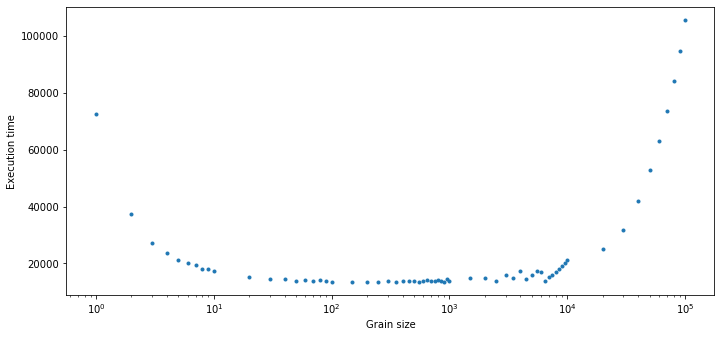
\includegraphics[scale=.45]{images/hpx_for_loop/100000_8.png}}
	\caption{The results of running the benchmark in Listing with $problem\_size=100,000$, on 8 cores. The unit for execution time is microseconds.}\label{fig41}		
\end{figure}


Since our proposed model does not depend on the $problem\_{size}$ but on the number of tasks created, number of cores, and the maximum amount of work assigned to a core, we are suggesting here that it might be sufficient to use the data collected from one $problem\_{size}$ to find the parameters $\alpha$ and $\gamma$. 

In order to test the viability of our proposition, we chose $problem\_{size}=100,000,000$ as a reasonable(not too small nor too large) base for our parameter estimation. Figure~\ref{fig42} shows the measured execution time in terms of grain size for $N=1,2,...,8$, with total $728$ points.
  
\begin{figure}[H]
	\centering
	{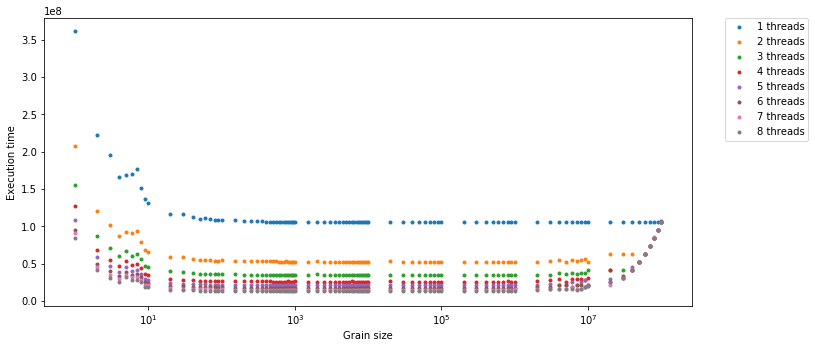
\includegraphics[scale=.45]{images/hpx_for_loop/100000000_8.png}}
	\caption{The results of running the benchmark in Listing with $problem\_size=100,000,000$, on 8 cores. The unit for execution time is microseconds.}\label{fig42}		
\end{figure}

Using all the $728$ data points for different number of cores, we used the $optimize.curve_fit$ package from $scipy$ library in Python to fit the collected data with our model, which resulted in $alpha=3.032$ and $\gamma=0.294$. $\alpha$ represents the overhead of creating associated with creating tasks in $\mu{secs}$, and $\gamma$ represents the contention.

\begin{figure}[H]
	\centering
	\subfloat[]
	{\centering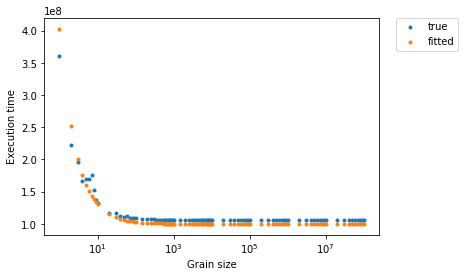
\includegraphics[scale=.4]{images/hpx_for_loop/fitted/100000000_1.png}	
		\label{fig43:a}}
	\subfloat[]
	{\centering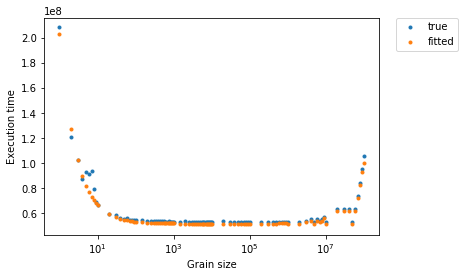
\includegraphics[scale=.4]{images/hpx_for_loop/fitted/100000000_2.png}	
	\label{fig43:b}}\hfill
	\subfloat[]
{\centering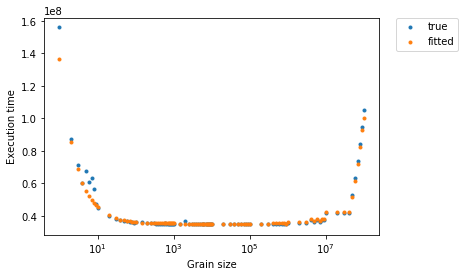
\includegraphics[scale=.4]{images/hpx_for_loop/fitted/100000000_3.png}	
	\label{fig43:c}}
\subfloat[]
{\centering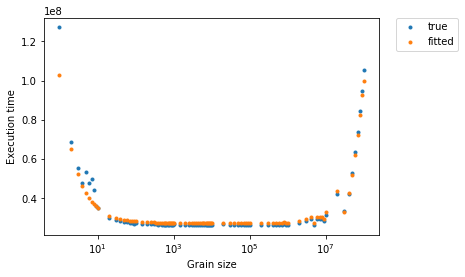
\includegraphics[scale=.4]{images/hpx_for_loop/fitted/100000000_4.png}	
	\label{fig43:d}}\hfill
	\subfloat[]
{\centering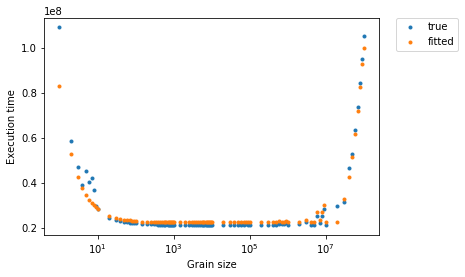
\includegraphics[scale=.4]{images/hpx_for_loop/fitted/100000000_5.png}	
	\label{fig43:e}}
\subfloat[]
{\centering\includegraphics[scale=.4]{images/hpx_for_loop/fitted/100000000_6.png}	
	\label{fig43:f}}\hfill
	\subfloat[]
{\centering\includegraphics[scale=.4]{images/hpx_for_loop/fitted/100000000_7.png}	
	\label{fig43:g}}
\subfloat[]
{\centering\includegraphics[scale=.4]{images/hpx_for_loop/fitted/100000000_8.png}	
	\label{fig43:h}}\hfill
	\caption{The results of predicted values of execution time through curve fitting vs the real data for with $problem\_size=100,000,000$, for (a) 1 core, (b) 2 cores, (c) 3 cores, (d) 4 cores, (e) 5 cores, (f) 6 cores, (g) 7 cores, (h) 8 cores.. The unit for execution time is microseconds.}
	\label{fig43}	
\end{figure}


Figure~\ref{fig43} shows the fitted curves along with the original data for different number of cores.
In order to measure how well the model is fitting the data we calculated the relative error as Formula~\ref{eq4}, where $p_i$ is the predicted value from curve fitting for sample $i$, $t_i$ is true value of that sample, and $n$ is the total number of samples.


\begin{equation}{\label{eq4}}
Relative\_{error} = \frac{1}{n}\sum_{i=1}^{n} {|1-\frac{p_i}{t_i}|}
\end{equation}

\begin{figure}[H]
	\centering
	{\includegraphics[scale=.45]{images/hpx_for_loop/fitted/marvin_relative_error_100000000.png}}
	\caption{The relative error of using the result of curve fitting for predicting the execution, for different number of cores, for $problem\_size=100,000$.}\label{fig44}		
\end{figure}



\begin{figure}[H]
	\centering
	{\includegraphics[scale=.45]{images/hpx_for_loop/fitted/marvin_relative_error_all.png}}
	\caption{The average relative error of using the result of curve fitting for $problem\_size=100,000,000$ for predicting the execution of different $problem\_{sizes}$ for different number of cores.}\label{fig45}		
\end{figure}

\begin{equation}{\label{eq5}}
R\textunderscore{squared} = 1-\frac{{\frac{1}{n}\sum_{i=1}^{n}{(t_i-p_i)}^2}}{Var(t)}
\end{equation}

\begin{figure}[H]
	\centering
	{\includegraphics[scale=.45]{images/hpx_for_loop/fitted/marvin_r2_error_all.png}}
	\caption{The average $R^2$ score of using the result of curve fitting for $problem\_size=100,000,000$ for predicting the execution of different $problem\_{sizes}$ for different number of cores.}\label{fig46}		
\end{figure}

At the next step we repeated the same process for the data collected from a different architecture, \textit{Medusa} node.
We used $problem\_{size}=1,000,000$, and after curve fitting the parameters $\alpha=1.793$ and $\gamma=0.279$ were obtained. The calculated mean relative error and mean $R^2$ measure for each individual number of cores is demonstrated in Figure~\ref{fig48}, and Figure~\ref{fig49}.

\begin{figure}[H]
	\centering
	\subfloat[]
	{\centering\includegraphics[scale=.4]{images/hpx_for_loop/fitted/medusa_1000000_1.png}	
		\label{fig50:a}}
	\subfloat[]
	{\centering\includegraphics[scale=.4]{images/hpx_for_loop/fitted/medusa_1000000_2.png}	
		\label{fig50:b}}\hfill
	\subfloat[]
	{\centering\includegraphics[scale=.4]{images/hpx_for_loop/fitted/medusa_1000000_3.png}	
		\label{fig50:c}}
	\subfloat[]
	{\centering\includegraphics[scale=.4]{images/hpx_for_loop/fitted/medusa_1000000_4.png}	
		\label{fig50:d}}\hfill
	\subfloat[]
	{\centering\includegraphics[scale=.4]{images/hpx_for_loop/fitted/medusa_1000000_5.png}	
		\label{fig50:e}}
	\subfloat[]
	{\centering\includegraphics[scale=.4]{images/hpx_for_loop/fitted/medusa_1000000_6.png}	
		\label{fig50:f}}\hfill
	\subfloat[]
	{\centering\includegraphics[scale=.4]{images/hpx_for_loop/fitted/medusa_1000000_7.png}	
		\label{fig50:g}}
	\subfloat[]
	{\centering\includegraphics[scale=.4]{images/hpx_for_loop/fitted/medusa_1000000_8.png}	
		\label{fig50:h}}\hfill
	\caption{The results of predicted values of execution time through curve fitting vs the real data for with $problem\_size=1,000,000$, for (a) 1 core, (b) 2 cores, (c) 3 cores, (d) 4 cores, (e) 5 cores, (f) 6 cores, (g) 7 cores, (h) 8 cores. The unit for execution time is microseconds.}
	\label{fig50}	
\end{figure}

\begin{figure}[H]
	\centering
	{\includegraphics[scale=.45]{images/hpx_for_loop/fitted/medusa_relative_error_100000.png}}
	\caption{The relative error of using the result of curve fitting for predicting the execution, for different number of cores, for $problem\_size=100,000$, on \textit{Medusa} node.}\label{fig47}		
\end{figure}



\begin{figure}[H]
	\centering
	{\includegraphics[scale=.45]{images/hpx_for_loop/fitted/medusa_relative_error_all.png}}
	\caption{The average relative error of using the result of curve fitting for $problem\_size=100,000,000$ for predicting the execution of different $problem\_{sizes}$ for different number of cores, on \textit{Medusa} node.}\label{fig48}		
\end{figure}

\begin{figure}[H]
	\centering
	{\includegraphics[scale=.45]{images/hpx_for_loop/fitted/medusa_r2_error_all.png}}
	\caption{The average $R^2$ score of using the result of curve fitting for $problem\_size=100,000,000$ for predicting the execution of different $problem\_{sizes}$ for different number of cores, on \textit{Medusa} node.}\label{fig49}		
\end{figure}

%\vspace{\baselineskip}	
%\begin{table}[H]
%	\centering
%	\resizebox{\textwidth}{!}
%	{\begin{tabular}{|c | c |} 
%			\hline
%			Category & Configuration \\
%			\hline
%			\hline
%		$Problem\_{size}$ & 100000 \\ [0.5ex] 
%			\hline
%			$N$ & 1, 2, 3, 4, 5, 6, 7, 8 \\ 	
%			\hline
%			$num\_{iterations}$ & 100000 \\
%			\hline	
%			$chunk\_{size}$ & 1,2,3,4,5,6,7,8,9,10,20,30,...,90000,100000 \\
%			\hline		
%	\end{tabular}}
%	
%	\caption{List of different configurations used for running the benchmark in Listing for $problem\_{size}=100000$}
%	\label{table6}
%\end{table}
   



\vspace{\baselineskip}
\subsection{Analyzing the Data}
Assuming the proposed formula is a good fit for this problem, we can estimate the range of grain sizes for which we achieve the lowest execution time, for a specific problem size, run on specific number of cores.

\vspace{\baselineskip}
\subsubsection{Left side of the graph}
As stated earlier, in Formula~\ref{formula1}, for small grain sizes the first term is the dominant factor while the second term roughly stays constant. Same way, for large grain sizes the second factor is the dominant factor. 

In order to find the lower-bound of the range for which the execution time stays constant, we assume the second factor is constant in that region. Also we can change $N$ to $M$, knowing that our concern is on the left hand side of the graph, where $num\_{tasks}$ is definitely greater than the number of cores. 
Taking the derivative of the function based on the grain size then leads to:

 
\begin{equation}\label{formula3}
\begin{aligned}
\frac{\partial execution\_{time}}{\partial g} &= \frac{\alpha}{N}\times{\frac{\partial num\_{tasks}}{\partial g}}+\delta\times{\frac{\partial num\_{tasks}}{\partial g}} \\
&=(\frac{\alpha}{N}+\delta)\times\frac{\partial(\frac{problem\_{size}}{g})}{\partial g} \\
&=(\frac{\alpha}{N}+\delta)\times{problem\_{size}}\times{\frac{-1}{g^2}}
\end{aligned}
\end{equation}

From Formula~\ref{formula3}, it can be observed that for the left hand side of the graph the rate of changes is negative and decreases as the grain size increases. Here we are looking for the value of the grain size for which the rate of change becomes very small (we introduce a threshold $\lambda_b$, where $\lambda_b\ll1$, for this purpose). 


\begin{equation}\label{formula4}
\begin{aligned}
&(\frac{\alpha}{N}+\delta)\times{problem\_{size}}\times{\frac{1}{g^2}}\leq{\lambda_b} \\
{g^2}&\geq{\frac{(\frac{\alpha}{N}+\delta)\times{problem\_{size}}}{\lambda_b}}\\
{g}&\geq{\sqrt{\frac{(\frac{\alpha}{N}+\delta)\times{problem\_{size}}}{\lambda_b}}}
\end{aligned}
\end{equation}

Formula~\ref{formula4} can also be represented as shown in Formula~\ref{formula5}. This representation shows that when the ratio of the time it takes to execute one task to the total overhead of creating and managing $num\_{tasks}$ tasks on $N$ core, is greater than a threshold, we will end up in the flat region of the graph, close to the left hand side.


\begin{equation}\label{formula5}
\begin{aligned}
(\frac{\alpha}{N}+\delta)\times{\frac{problem\_{size}}{g}}\times{\frac{1}{g}}&\leq{\lambda_b}\\
(\frac{\alpha}{N}+\delta)\times{num\_{tasks}}\times{\frac{1}{g}}&\leq{\lambda_b}\\
(\frac{\alpha}{N}+\delta)\times{num\_{tasks}}&\leq{g\times\lambda_b}\\	
\frac{g}{(\frac{\alpha}{N}+\delta)\times{num\_{tasks}}}&\geq{\frac{1}{\lambda_b}}
\end{aligned}
\end{equation}


\subsubsection{Right side of the graph}
Now looking at the right hand side of the graph, the overhead of creating the tasks becomes negligible on that side, since only few tasks are being created and the overhead of creating these many tasks is not significant compared to the execution time. On this side, the maximum amount of work executed by one core ($w\_c$) is the dominant factor.

Formula~\ref{formula2} shows how $w\_c$ is calculated for different cases, but in general we can estimate $w\_c$ with $g\times\left \lceil{\frac{num\_{tasks}}{N}}\right \rceil$. 

\begin{equation}\label{formula6}
\begin{aligned}
w\_c&\approx{g\times\left \lceil{\frac{num\_{tasks}}{N}}\right \rceil}\\
&\approx{g\times\left \lceil{\frac{\frac{problem\_{size}}{g}}{N}}\right \rceil}\\
&\approx{\frac{problem\_{size}}{N}} \:\:\text{\:\:\:\:if\:\:} num\_{tasks}\geq{N}
\end{aligned}
\end{equation}

What happens here is that as the grain size changes, there are points for which $\left \lceil{\frac{num\_{tasks}}{N}}\right \rceil$ is the same but since the grain size is different, a different $w\_c$ would be resulted. 
For all the values of $g$ that create the same $\left \lceil{\frac{num\_{tasks}}{N}}\right \rceil$, as $g$ increases the difference between $w\_c$ and $\frac{problem\_{size}}{N}$ increases. 

For example, considering a case where $problem\_{size}=100,000$, and $N=8$, for the grain sizes in range of $[4167,\:6249]$ would result in creating between $\left \lceil{\frac{100,000}{6,249}}\right \rceil=17$ and  $\left \lceil{\frac{100,000}{4,167}}\right \rceil=24$ tasks. This amount of tasks created itself would result in $\left \lceil{\frac{17}{8}}\right \rceil=3$ and  $\left \lceil{\frac{24}{8}}\right \rceil=3$ tasks.
On the other hand, $w\_c=g\times{\left \lceil{\frac{num\_{tasks}}{N}}\right \rceil}=3\times{g}$, would have a value in range of $[3\times4167,\:3\times6249]=[12501,\: 18747]$, where the average amount of work per core is $\frac{problem\_{size}}{N}=12500$. This means that for grain sizes closer to the end of the range, we are observing that a much bigger amount of work is assigned to the core with maximum amount of work, which would result in a higher execution time. 


In the general case, if we denote $\left \lceil{\frac{num\_{tasks}}{N}}\right \rceil$ as $k$, then:


\begin{equation}\label{formula8}
\begin{aligned}
k-1&<{\frac{num\_{tasks}}{N}}\leq{k}\\
(k-1)\times{N}&<num\_{tasks}\leq{k}\times{N}\\
%num\_{tasks}=\left \lceil{\frac{problem\_{size}}{g}}\right \rceil\\
(k-1)\times{N}&<\left \lceil{\frac{problem\_{size}}{g}}\right \rceil\leq{k}\times{N}\\
(k-1)\times{N}&<\frac{problem\_{size}}{g}\leq{{k}\times{N}}\\
\end{aligned}
\end{equation}

If $k=1$, then, 

\begin{equation}\label{formula9}
\begin{aligned}
0<\frac{problem\_{size}}{g}\leq{N}\\
\frac{problem\_{size}}{N}\leq{g}\leq{problem\_{size}}.
\end{aligned}
\end{equation}

Otherwise, when $k>1$,

\begin{equation}\label{formula10}
\begin{aligned}
\frac{problem\_{size}}{k\times{N}}\leq{g}<\frac{problem\_{size}}{(k-1)\times{N}}.
\end{aligned}
\end{equation}

Since $\left \lceil{\frac{num\_{tasks}}{N}}\right \rceil=k$, and $w\_c={g\times\left \lceil{\frac{num\_{tasks}}{N}}\right \rceil}={k\times{g}}$ if $num\_{tasks}\%{N}\neq{1}$, we can conclude for $k>1$:

\begin{equation}\label{formula11}
\begin{aligned}
k\times{\frac{problem\_{size}}{k\times{N}}}&\leq{w\_c}<{k\times{\frac{problem\_{size}}{(k-1)\times{N}}}}\\
\frac{problem\_{size}}{{N}}&\leq{w\_c}<{\frac{k}{k-1}\times{\frac{problem\_{size}}{N}}}\\
0&\leq{w\_c-\frac{problem\_{size}}{N}}<\frac{1}{k-1}\times{\frac{problem\_{size}}{N}}
\end{aligned}
\end{equation}

For the cases where $k>1$ and $num\_{tasks}\%{N}={1}$, there could be a  change in $w\_c$ if $problem\_{size}\%{g}\neq{0}$. For these cases:


\begin{equation}\label{formula15}
\begin{aligned}
\left \lceil{\frac{num\_{tasks}}{N}}\right \rceil&=k \text{\:\:\:}\&\text{\:\:\:} num\_{tasks}\%{N}={1}\Rightarrow\\
num\_{tasks}&=(k-1)\times{N}+1\Rightarrow\\
(k-1)\times{N}&<{\frac{problem\_{size}}{g}}\leq(k-1)\times{N}+1\Rightarrow\\
\frac{problem\_{size}}{(k-1)\times{N}+1}&\leq{g}<\frac{problem\_{size}}{(k-1)\times{N}}
\end{aligned}
\end{equation}

From Formula~\ref{formula2} we know,
\begin{equation}\label{formula17}
\begin{aligned}
w\_c={problem\_{size}}-(k-1)\times(N-1)\times{g}.
\end{aligned}
\end{equation}

Therefore,
\begin{equation}\label{formula18}
\begin{aligned}
(k-1)(N-1)\frac{problem\_{size}}{(k-1){N}+1}&\leq{(k-1)(N-1){g}}<(k-1)(N-1)\frac{problem\_{size}}{(k-1){N}}\Rightarrow\\
{\frac{problem\_{size}}{N}}&<{problem\_{size}-{(k-1)(N-1){g}}}\leq{k\frac{problem\_{size}}{(k-1){N}+1}}\\
{\frac{problem\_{size}}{N}}&<{w\_{c}}\leq{k\times\frac{problem\_{size}}{(k-1){N}+1}}
\end{aligned}
\end{equation}

And for $k=1$, where $num\_{tasks}\leq{N}$,
\begin{align*}\label{formula12}
w\_c&=g\\
\frac{problem\_{size}}{N}&\leq{g}\leq{problem\_{size}}\Rightarrow
\end{align*}

\begin{equation}\label{formula14}
\begin{aligned}
0\leq{w\_c-\frac{problem\_{size}}{N}}={g-\frac{problem\_{size}}{N}}\leq(N-1)\times{\frac{problem\_{size}}{N}}\\
\end{aligned}
\end{equation}


Defining $imbalance\_{ratio}=\frac{w\_c-\frac{problem\_{size}}{N}}{\frac{problem\_{size}}{N}}$, then,

\begin{equation}\label{formula13}
\begin{aligned}
0&\leq{imbalance\_{ratio}}\leq{N-1}  \text{\:\:\:\:\:\:\:\:\:\:\:\:\:for\:\:\:}k={1}\\
0&\leq{imbalance\_{ratio}}<\frac{1}{k-1}  \text{\:\:\:\:\:\:\:\:\:\:\:\:\:for\:\:\:}k>{1} \text{\:\:and\:\:}num\_{tasks}\%{N}\neq{1}\\
0&\leq{imbalance\_{ratio}}<\frac{N-1}{N(k-1)+1}=\frac{1}{k-1+\frac{k}{N-1}}\text{\:\:\:\:\:\:\:\:\:\:\:\:\:otherwise}
\end{aligned}
\end{equation}

%k\in\mathbb{Z}
Formula~\ref{formula13} shows that as number of created tasks increases, as long as number of tasks per core is the same, the imbalance factor decreases. 

\vspace{\baselineskip}

Figure~\ref{fig38} shows the imbalance ratio calculated for different grain sizes for $problem\_size=10000$, on 8 cores. Each of the regions between two dashed green lines correspond to a specific value for $k=\left\lceil{\frac{num\_{tasks}}{N}}\right \rceil$. 
At each of the regions with $k>1$, $\left\lceil{\frac{num\_{tasks}}{N}}\right \rceil=k$,  $imbalance\_{ratio}$ starts from $0$ and approaches $\frac{1}{k-1}$ ($\frac{1}{k-1+\frac{k}{N-1}}$ for regions where $num\_{tasks}\%{N}\neq{1}$) at the end of the region. When $k=1$, $imbalance\_{ratio}$ increases linearly starting from 0 and reaching the maximum of $N-1$ when $g=pronblem\_{size}$. As we move to larger grain sizes, $\left\lceil{\frac{num\_{tasks}}{N}}\right \rceil$ decreases, therefore the upper-bound for $imbalance\_{ratio}$ increases.   


\vspace{\baselineskip}	
\begin{figure}[H]
	\centering
	{\includegraphics[scale=.25]{images/hpx_for_loop/w_c_all.png}}
	\caption{The imbalance ratio calculated for different grain sizes for $problem\_size=10000$, on 8 cores, where $k=\left\lceil{\frac{num\_{tasks}}{N}}\right \rceil$.}\label{fig38}		
\end{figure}


%\vspace{\baselineskip}	
%\begin{figure}[H]
%	\centering
%	{\includegraphics[scale=.45]{images/hpx_for_loop/max_w_c.png}}
%	\caption{The maximum imbalance ratio calculated for different grain sizes for $problem\_size=10000$, on 8 cores, where $k=\left\lceil{\frac{num\_{tasks}}{N}}\right \rceil$.}\label{fig36}		
%\end{figure}

Figure~\ref{fig39} represents the imbalance ratio, along with the ratio of the sequential execution time over execution time(speed-up) against grain size for $problem\_size=10000$, ran on 8 cores.   
As it can be observed, as the $imbalance\_{ratio}$ increases, the speed-up decreases. 

\vspace{\baselineskip}	
\begin{figure}[H]
	\centering
	{\includegraphics[scale=.3]{images/hpx_for_loop/w_c_speedup.png}}
	\caption{The imbalance ratio calculated for different grain sizes for $problem\_size=10000$, on 8 cores, where $k=\left\lceil{\frac{num\_{tasks}}{N}}\right \rceil$.}\label{fig37}		
\end{figure}


To summarize, as the grain size increases the maximum imbalance in the loads assigned to the cores also increases, and some point on, this imbalance has a significant affect in the execution time. We define a threshold, $\lambda_s$ ($0<\lambda_s<1$), where for $imbalance\_{ratio}$s smaller than this threshold the imbalance effect is not significant. As we get close to this threshold, we are likely to reach the right hand side of the flat region of the bathtub curve of the execution time against grain size. 


We are interested in finding the maximum grain size that would generate a reasonable imbalance ($imbalance\_{ratio}\leq{\lambda_s}$), to make sure we should stay in the flat region of the bathtub curve of execution time against grain size, from load imbalance point of view.  

Formula~\ref{formula14} states that for grain sizes greater than $problem\_{size}$, $imblance\_{ratio}$ increases linearly with grain size from $0$ to $N-1$. While for grain sizes smaller than $problem\_{size}$, the maximum $imbalance\_{ratio}$ depends on $k=\left\lceil{\frac{num\_{tasks}}{N}}\right\rceil$. So, in order to assure \emph{imbalance\_{ratio}} is smaller than or equal to a threshold ($\lambda_s$), first we search the grain sizes smaller than $\frac{problem\_{size}}{N}$. Since $0<\lambda_s<1$, and $k\geq2$ in this region, there exists a $k$ such that $\frac{1}{k-1}\leq\lambda_s$.    
If there exists a $k_{min}$ (creating an imbalance ratio between $0$ and $\frac{1}{k_{min}-1}$), where $\frac{1}{k_{min}-1}\leq{\lambda_s}$, $\forall k<k_{min}$ maximum value of $imbalance\_{ratio}$ would be greater than $\lambda_s$. So in order to find the grain size that would create maximum $imbalance\_{ratio}$ of $\lambda_s$:



\begin{equation}\label{formula21}
\begin{aligned}
&imbalance\_{ratio}\leq{{\lambda_s}}\Rightarrow\\
&\frac{1}{k-1}\leq\lambda_s\\
&k\geq{1+\frac{1}{\lambda_s}}\\
&k_{min}=\left\lceil{1+\frac{1}{\lambda_s}}\right\rceil+1\\
&{g}<\frac{problem\_{size}}{(k_{min}-1)\times{N}}\\
&g_{max}=\frac{problem\_{size}}{(k_{min}-1)\times{N}}-1=\frac{problem\_{size}}{(1+\left\lceil{\frac{1}{\lambda_s}}\right\rceil)\times{N}}
\end{aligned}
\end{equation}

If $g<g\_{max}$, we can assure that $imbalance\_{ratio}$ never exceeds $\lambda_s$. Since we already found a match at grain sizes smaller than $\frac{problem\_{size}}{N}$, checking the rest of grain sizes would not be necessary.





\begin{lstlisting}[basicstyle=\fontsize{8}{9}\selectfont,float,floatplacement=H,caption= {A simple hpx for\textunderscore{loop} used to study the effect of grain size on the achieved parallelism.}, label={hpx_for_loop}]

///////////////////////////////////////////////////////////////////////////////
void measure_function_futures_for_loop(std::uint64_t count, bool csv, std::uint64_t chunk_size, std::uint64_t iter_length)
{
// start the clock
high_resolution_timer walltime;
hpx::parallel::for_loop(hpx::parallel::execution::par.with(
hpx::parallel::execution::dynamic_chunk_size( chunk_size )),
0, count, [&](std::uint64_t) { worker_timed(iter_length*1000); });
// stop the clock
const double duration = walltime.elapsed();
print_stats("for_loop", "par", "parallel_executor", count, duration, csv);
}

///////////////////////////////////////////////////////////////////////////////
int hpx_main(variables_map& vm)
{
{
const int repetitions = vm["repetitions"].as<int>();
num_threads = hpx::get_num_worker_threads();
const std::uint64_t chunk_size = vm["chunk_size"].as<std::uint64_t>();
const std::uint64_t iter_length = vm["iter_length"].as<std::uint64_t>();
const std::uint64_t count = vm["num_iterations"].as<std::uint64_t>();
bool csv = vm.count("csv") != 0;
if (HPX_UNLIKELY(0 == count))
throw std::logic_error("error: count of 0 futures specified\n");
for (int i = 0; i < repetitions; i++)
{
measure_function_futures_for_loop(count, csv, chunk_size, iter_length);
}
}
return hpx::finalize();
}
///////////////////////////////////////////////////////////////////////////////
inline void worker_timed(std::uint64_t delay_ns)
{
if (delay_ns == 0)
return;
std::uint64_t start = hpx::util::high_resolution_clock::now();
while (true)
{
// Check if we've reached the specified delay.
if ((hpx::util::high_resolution_clock::now() - start) >= delay_ns)
break;
}
}
///////////////////////////////////////////////////////////////////////////////
int main(int argc, char* argv[])
{
// Configure application-specific options.
options_description cmdline("usage: " HPX_APPLICATION_STRING " [options]");
cmdline.add_options()("num_iterations",
value<std::uint64_t>()->default_value(500000),
"number of iterations to invoke")
("repetitions", value<int>()->default_value(1),
"number of repetitions of the full benchmark")
("iter_length",value<std::uint64_t>()->default_value(1), "length of each iteration")
("chunk_size",value<std::uint64_t>()->default_value(1), "chunk size");
// Initialize and run HPX.
return init(cmdline, argc, argv);
}
\end{lstlisting}

\vspace{\baselineskip}
\subsection{Identifying the range of grain size for maximum speedup}
In the previous section, we proposed a method to identify the lower-bound and the upper-bound of the grain sizes for which we observe the minimum execution time. 
Integrating Formula~\ref{formula4} and Formula~\ref{formula21} suggests the following range for maximum speedup:


\begin{equation}\label{formula23}
\begin{aligned}
{\sqrt{\frac{(\frac{\alpha}{N}+\delta)\times{problem\_{size}}}{{\lambda_b}}}}\leq{g}\leq\frac{problem\_{size}}{(1+\left\lceil{\frac{1}{\lambda_s}}\right\rceil)\times{N}}
\end{aligned}
\end{equation}
 
Where $0\leq\lambda_s\leq1$, and $\lambda_b,\lambda_s\ll1$.

In this section we represent the identified range for a number of problem sizes, with different number of cores.


%\vspace{\baselineskip}
%\subsection{Analyzing the Data}
%Throughout these experiments we try to fix or eliminate the factors we believe will affect the execution time as much as possible, study the results, and then introduce one factor to the model and study the behavior of the model. 



\vspace{\baselineskip}
%\subsection{Step 1: Sequential Run}
%In the first step in order to eliminate all the factors related to parallel execution we run the code sequentially for some problem sizes. The obtained result, as shown in Figure~\ref{fig26} demonstrates an overhead that increases as the number of iterations increases.
%
%\begin{figure}
%	\centering
%	\includegraphics[width=1\linewidth]{images/hpx_for_loop/overheads_seq.png}
%	\caption{The results obtained from running the hpx for loop sequentially}	
%	\label{fig26}
%\end{figure}




\vspace{\baselineskip}

\clearpage

\subsection{Step 1: Single-task, single-core runs}
At the first step, we look at the cases where only one task has been created, the program is run on only one core. This problem could be assumed to be equivalent to running the same amount of work sequentially with an additional cost of creating just one task. 
\subsubsection{Expected Model}
With this assumption we expect the execution time to be summation of the time it takes to perform the total amount of work(\textit{problem\textunderscore{size}}) and the overhead of creating one HPX task($\alpha$). Formula~\ref{chunk1} shows the expected formula.

\begin{equation}\label{chunk1}
execution\:\:time = \alpha + problem\:\:size
\end{equation}  

\vspace{\baselineskip}
\subsubsection{Original Data}
In order to check our proposed model for this simplified problem, we collected data from running the program, setting the \textit{chunk\textunderscore{size}} to 1, \textit{num\textunderscore{iterations}} to 1, and changing the \textit{iter\textunderscore{length}} from 1 to 10,000,000. 




%To summarize, knowing the grain size, we are expecting the execution time in a many-task runtime system to be mainly affected by these factors, the overhead of creating one task($\alpha$), the number of cores that are actually doing the work($M$), the sequential execution time($t_s$), and finally the portion of the program that could actually be parallelized($\gamma$). 
%
%If we try to integrate these information into a formula, we would expect the relation between execution time($t$) and number of tasks($n_t$) as follows:
%\begin{equation}\label{new1}
%t=\frac{\alpha{n_t}+t_s}{M}+\gamma
%\end{equation}
%
%which could be decomposed into these two equations:
%
%
%Now we use this function to find the best three parameters $\alpha$, $t_s$, and $\gamma$ so that the collected data would fit this model. For this purpose we used the \textit{curve\textunderscore{fit}} package from \textit{SciPy} library in \textit{python}.
%
%In order to make Equation~\ref{new1} differentiable, we used the softplus function(Equation~\ref{softplus1}) to represent $M$ based on $n_t$.
%\begin{equation}\label{softplus1}
%f(x)=Ln(1+e^x)
%\end{equation}
%
%Which results in Equation~\ref{soft_plus1}:
%\begin{equation}\label{soft_plus1}
%t=\frac{\alpha{n_t}+t_s}{(N-1)-Ln(1+(e^{N-1}-1)e^{-n_t})}+\gamma
%\end{equation}




\vspace{\baselineskip}
\pagebreak
\singlespacing

\chapter{Setup}\label{Results}
\doublespacing
\section{Setup}
Our experiments were run on Marvin nodes of Rostam cluster at Center for Computation and Technology(CCT) at Louisiana State University. Table~\ref{table3} and Table~\ref{4} show some of the specifications of this node.

\vspace{\baselineskip}	
\begin{table}[H]
	\centering
%	\resizebox{\textwidth}{!}
	\scalebox{0.75}
	{\begin{tabular}{|c | c |} 
			\hline
			CPU &  2 x Intel(R) Xeon(R) CPU E5-2450 0 @ 2.10GHz \\ [0.5ex] 
			\hline
			RAM & 48 GB\\ 	
			\hline
			Number of Cores & 16\\
			\hline	
			Hyperthreading & Off \\
			\hline			
	\end{tabular}}	
	\caption{Specifications of the Marvin node from Rostam cluster at CCT.}
	\label{table3}
\end{table} 


\vspace{\baselineskip}	
\begin{table}[H]
	\centering
	\scalebox{0.9}
	{\begin{tabular}{|c | c | c | c | c|} 
			\hline
			Cache Level &  Coherency Line Size & Number of Sets & Ways of Associativity & Size\\ [0.5ex] 
			\hline
			1 & 64 & 512 & 8 & 32KB \\	
			\hline
			2 & 64 & 512 & 8 & 256KB \\
			\hline	
			3 & 64 & 512 & 20 & 20480KB \\
			\hline			
	\end{tabular}}	
	\caption{Cache specifications of the Marvin node from Rostam cluster at CCT.}
	\label{table4}
\end{table} 
\vspace{\baselineskip}	

%Marvin:
%cache level 1
%coherency line size: 64
%number of sets: 512
%ways of associativity: 8
%type: Instruction
%size: 32K
%
%cache level 2
%coherency line size: 64
%number of sets: 512
%ways of associativity: 8
%type: Unified
%size: 256K
%
%cache level 3
%coherency line size: 64
%number of sets: 512
%ways of associativity: 20
%type: Unified
%size: 20480K
%
%
%Trillian:
%cache level 1
%coherency line size: 64
%number of sets: 64
%ways of associativity: 4
%type: Data
%size: 16K
%
%cache level 1
%coherency line size: 64
%number of sets: 512
%ways of associativity: 2
%type: Instruction
%size: 64K
%
%cache level 2
%coherency line size: 64
%number of sets: 2048
%ways of associativity: 16
%type: Unified
%size: 2048K

%cache level 3
%coherency line size: 64
%number of sets: 2048
%ways of associativity: 48
%type: Unified
%size: 6144K



\pagebreak
\singlespacing

\chapter{Proposed Study}\label{Future}
\doublespacing
\section{What is the role of matrix size?}
In Chapter~\ref{Method} two different functions were proposed to model the relationship between grain size, number of cores, and performance (execution time or throughput). These functions were fitted for each matrix size individually for simplification, but this assumption is not practical, since even though the characteristics of the function is the same for all matrix sizes, the fitted parameters vary from one matrix size to another. 

The matrix size should somehow be integrated into the model itself. For this purpose, first we need to understand how changing the matrix size affects the relationship between grain size and performance. 
One immediate effect of increasing the matrix size is an increase in maximum possible grain size (right hand side of Figure~\ref{fig19} ) , while the minimum possible grain size is the same.

\vspace{\baselineskip}	
\begin{figure}[H]	
	\centering\includegraphics[scale=.75]{images/fig11.png}			
	\caption{Throughput vs. grain size graph obtained from running $DMATDMATADD$ benchmark  on $4$ cores.}
	\label{fig19}	
\end{figure} 


Moreover, Figure~\ref{fig20} shows how the predicted grain size range changes for different matrix sizes.
 
\vspace{\baselineskip}	
\begin{figure}[H]	
	\centering\includegraphics[scale=.75]{images/polyfit/fig_all_sizes_range_silver.png}			
	\caption{The predicted range of grain size for maximum performance for different matrix sizes, using polynomial fit, based on $DMATDMATADD$ benchmark.}
	\label{fig20}	
\end{figure} 
\pagebreak
\singlespacing

\chapter{Appendix}
\doublespacing
\section{Bathtub model}
In the previous section we studied the possibility of using a polynomial to capture the relationship between grain size, number of cores, and throughput for a fixed matrix size, with the purpose of finding a range of grain size that leads us to maximum performance. 
Although the polynomial function was helpful in directing us toward our objective, it does not have a physical implication. 

This motivated us to change our view, and instead of looking just at the data and trying to find a function to fit the data, study the behavior of the data, and then find a function that would be likely to fit the data. That function would be a good fit mostly because that's how we expect the throughput to change with grain size, and not just how the data looks like.   

As stated in Section~\ref{task}, Grubel et.al.\cite{grubel2015performance} has studied the task granularity for a specific problem(1D stencil). Looking at the graph representing the execution time based on the grain size, which resembles a bathtub, we are interested in formulating this graph based on our understanding of the effect of task granularity. Figure~\ref{fig21} shows the execution time in terms of grain size for $DMATDMATADD$ benchmark for matrix size $690\times690$ on $4$ cores.

\vspace{\baselineskip}	
\begin{figure}[H]
	\centering
	\subfloat[]{\includegraphics[scale=.5]{images/bathtub/all_690_4.png}\label{fig20:a}}
	\subfloat[]{\includegraphics[scale=.5]{images/bathtub/tasks_all_690_4.png}\label{fig20:b}}
	\caption{(a)The execution time vs. grain size graph, and (b) execution time vs. number fo tasks graph for $DMATDMATADD$ benchmark for matrix size $690\times690$ ran on $4$ cores.}	
	\label{fig21}
\end{figure}

\vspace{\baselineskip}	
For the sake of simplicity, we change the x axis from grain size to number of tasks. Each specific grain size would create a specific number of tasks(HPX threads), since the parameters we are interested in are directly associated with he number of tasks, we represent execution time based on number of tasks, as shown in Figure~\ref{fig20:b}.
 

Looking at the left hand side of the graph in Figure~\ref{fig20:b}, we can observe that for the first three points, the number of tasks created is smaller than the number of cores(which is 4 in this example). This means that in any of these cases there is at least one idle core, while the other cores are assigned a rather big chunk of work. The performance degradation we observe in that points is associated with starvation, meaning that we are not utilizing our computation resources to the full extent. In these three points, the number of cores actually doing the work is equal to the number of the tasks, since each core gets to execute at most one task.    

To generalize the problem, assuming we are running our application on $N$ cores, with a grain size equal to $g$, $n_t$ tasks are being created, and $M$ cores are actually doing the work. If $n_t<N$, $M$ would be equal to $n_t$, otherwise $M=N$.


From overhead point of view though, if we represent the overhead of creating one task on a particular machine as $\alpha$, the overhead of creating $d$ tasks would be $n_t\alpha$, but this overhead is divided between the $M$ cores actually doing the work. 

To summarize, knowing the grain size, we are expecting the execution time in a many-task runtime system to be mainly affected by these factors, the overhead of creating one task($\alpha$), the number of cores that are actually doing the work($M$), the sequential execution time($t_s$), and finally the portion of the program that could actually be parallelized($\gamma$). 

If we try to integrate these information into a formula, we would expect the relation between execution time($t$) and number of tasks($n_t$) as follows:
\begin{equation}\label{new}
t=\frac{\alpha{n_t}+t_s}{M}+\gamma
\end{equation}

which could be decomposed into these two equations:

\begin{equation}
t=\left\{
\begin{aligned}
\alpha+\frac{t_s}{n_t}+\gamma  \:\:\:\:\:\:\:\:      \text{ if } n_t<N\\
\frac{\alpha{n_t}+t_s}{N}+\gamma\:\:\:\:\:\:\:\:     \text{otherwise}
\end{aligned}
\right.
\end{equation}

Now we use this function to find the best three parameters $\alpha$, $t_s$, and $\gamma$ so that the collected data would fit this model. For this purpose we used the \textit{curve\textunderscore{fit}} package from \textit{SciPy} library in \textit{python}.

In order to make Equation~\ref{new} differentiable, we used the softplus function(Equation~\ref{softplus}) to represent $M$ based on $n_t$.
\begin{equation}\label{softplus}
f(x)=Ln(1+e^x)
\end{equation}

Which results in Equation~\ref{soft_new}:
\begin{equation}\label{soft_new}
t=\frac{\alpha{n_t}+t_s}{(N-1)-Ln(1+(e^{N-1}-1)e^{-n_t})}+\gamma
\end{equation}

Here again we limited our problem to one specific matrix size at a time, and divided the whole data for each matrix size and number of cores into two parts, $60\%$ for training and $40\%$ for testing.


\vspace{\baselineskip}	
\begin{figure}[H]
	\centering
	\subfloat[]{\includegraphics[scale=.45]{images/bathtub/pred/pred_690_4.png}\label{fig22:a}}
	\subfloat[]{\includegraphics[scale=.45]{images/bathtub/pred/pred_690_8.png}\label{fig22:b}}	
	\caption{The prediction of execution time based on grain size using the bathtub model, for (a)4 cores and (b)8 cores for $DMATDMATADD$ benchmark for matrix size $690\times690$.}	
	\label{fig22}
\end{figure}
\vspace{\baselineskip}	
Figure~\ref{fig23} represents the relative error calculated for both training and test set, which is less than $5\%$.

\vspace{\baselineskip}	
\begin{figure}[H]
	\centering
	{\includegraphics[scale=.45]{images/bathtub/error_690.png}}	
	\caption{The error in fitting execution time with the bathtub formula for $DMATDMATADD$ benchmark for matrix size $690\times690$ with different number of cores.}	
	\label{fig23}
\end{figure}

\vspace{\baselineskip}	
Assuming that this function fits our data in acceptable manner, next step would be to check how these three parameters change with the number of cores.

\begin{equation}\label{usl_fit}
f(x)=\frac{m_0}{x}+\frac{m_1(x-1)}{x}+m_2(x-1)+m_3(x)(x-1)
\end{equation}


\vspace{\baselineskip}	
\begin{figure}[H]
	\centering
	\subfloat[]{\includegraphics[scale=.3]{images/bathtub/coef_1_690.png}\label{fig24:a}}
	\subfloat[]{\includegraphics[scale=.3]{images/bathtub/coef_2_690.png}\label{fig24:b}}	
	\subfloat[]{\includegraphics[scale=.3]{images/bathtub/coef_3_690.png}\label{fig24:c}}
	\caption{Fitting the three parameters (a)$\alpha$, (b)$t_s$, and (c)$\gamma$ for $DMATDMATADD$ benchmark for matrix size $690\times690$.}	
	\label{fig24}
\end{figure}


\vspace{\baselineskip}	
We can integrate Equation~\ref{new} and Equation~\ref{usl_fit} to predict the execution time for a given matrix size and number of cores.
For each matrix size having found the parameters $m_0$ to $m_3$, we can find $\alpha$, $t_s$, and $\gamma$ for the particular number of cores requested through Equation~\ref{usl_fit}. Then we can plug in the calculated values for $\alpha$, $t_s$, and $\gamma$ into Equation~\ref{new} to predict the execution time.

Figure~\ref{fig25} shows the prediction error on the test set for $DMATDMATADD$ benchmark for matrix size $690\times690$. The axis shows the different samples in the test set, and the label of each point represents the number of tasks created for that particular data point. As it could be seen, certain number of tasks result in higher prediction error, which needs to be studied.


\vspace{\baselineskip}	
\begin{figure}[H]
	\centering	{\hfill\includegraphics[scale=.35]{images/bathtub/prediction_error_overall690.png}}	
	\caption{The error in fitting execution time with the bathtub formula for $DMATDMATADD$ benchmark for matrix size $690\times690$ with different number of cores.}	
	\label{fig25}
\end{figure}

The problem with the current model is that with this formula we know that the minimum occurs at $n_t=N$, but that's not usually the case. This inspires us to check for a missing factor. 
This model still needs to be studied. The estimate that we have is for execution time, which is in our experiments very small. Changing the graphs from execution time to throughput can help us find the location of the maximum throughput easier compared to minimum of the execution time.


\subsection{Studying the effect of matrix size}


\pagebreak
\singlespacing

%To insert additional chapters, copy the previous five lines, using chapterX as the argument of the 
%\input command for Chapter X, where X=6,7,8,...
\addtocontents{toc}{\vspace{12pt}}
\addcontentsline{toc}{chapter}{\hspace{-1.6em} REFERENCES}
%\begin{thebibliography}{999}
\vspace{0.9em}
\bibliographystyle{unsrt}
\bibliography{bibliography}
%\input{bibliography}
%\end{thebibliography}


\addtocontents{toc}{\vspace{12pt} \hspace{-1.8em} APPENDIX \vspace{-1em}}
\pagebreak
\singlespacing
\appendix
%\chapter{Copyright Information}
%\vspace{0.5em}
%\input{appendixA}
%\pagebreak
%\addtocontents{toc}{\vspace{12pt} \hspace{-1.8em} APPENDIX \vspace{-1em}}
%\appendix
%\chapter{Title of Appendix A}
%\vspace{0.5em}
%\input{appendixA}
%\pagebreak
%\chapter{Title of Appendix B}
%\vspace{0.5em}
%\input{appendixB}
%\pagebreak
%If you need to insert additional appendices, copy the previous four lines, using appendixY as the
%argument of the \input commnd for Appendix Y, for Y=C,D,E,...

%Finally, the vita section is created and included in the Table of Contents.
%\chapter*{Vita}
%\doublespacing
%\setlength{\parindent}{1.75em}
%\vspace{0.2em}
%\addtocontents{toc}{\vspace{12pt}}
%\addcontentsline{toc}{chapter}{\hspace{-1.5em} VITA}
%Insert the text of your vita, which is basically a description of yourself and your academic career.
%\singlespacing
%\chapter*{Vita}
%\doublespacing
%\setlength{\parindent}{1.75em}
%\vspace{0.2em}
%\addtocontents{toc}{\vspace{12pt}}
%\addcontentsline{toc}{chapter}{\hspace{-1.5em} VITA}
%VITA
\end{document}





